		\PassOptionsToPackage{svgnames}{xcolor}
\documentclass[a4paper,twoside,10pt]{article}
\usepackage[utf8]{inputenc}
\usepackage{hyperref}
\hypersetup{
	colorlinks,
	citecolor=black,
	filecolor=black,
	linkcolor=black,
	urlcolor=black
}
\usepackage{enumitem}
\usepackage{tipfr}
\usepackage{framed}
\usepackage{babel}
\usepackage{graphicx}
\usepackage{amssymb}
\usepackage{amsfonts}
\usepackage{amsmath}
\usepackage{pgfplots}
\usepackage{amsmath}
\usepackage{centernot}
\usepackage{mathrsfs}
\usepackage{tikz}
\usepackage{tkz-euclide}
\usepgfplotslibrary{polar}
\usepgfplotslibrary{fillbetween}
\usetikzlibrary{pgfplots.polar}
\pgfplotsset{compat=1.18, width=\textwidth}
\usepackage{mathtools}
\usepackage[thinc]{esdiff}
\def\pgfplots@stacked@diff{}
\setlength\parindent{12pt}
\usepackage{tabularx}
\usepackage{makecell}
\usepackage{amsthm}
\usepackage{tabularx}
\usepackage[noEnd=true]{algpseudocodex}
\usepackage{algorithm}
\usepackage[a4paper, marginparwidth=80pt, top=2cm, bottom=1cm, left=2cm, right=0.5cm]{geometry}
\usepackage{marginnote}
\usepackage{polynom}
\usepackage{xfrac}
\usepackage{gensymb}
\usepackage{fancyhdr}
\usepackage{undertilde}
\usepackage{nicematrix}
\usepackage{float}
\usepackage{ragged2e}
\usepackage{graphicx}
\usepackage{tcolorbox}
\usepackage{lipsum}
\tcbuselibrary{skins,breakable}
\graphicspath{{./img/}}
\usepackage{mathrsfs}
\newsavebox\foobox
\newlength{\foodim}
\newcommand{\slantbox}[2][0]{\mbox{%
		\sbox{\foobox}{#2}%
		\foodim=#1\wd\foobox
		\hskip \wd\foobox
		\hskip -0.5\foodim
		\pdfsave
		\pdfsetmatrix{1 0 #1 1}%
		\llap{\usebox{\foobox}}%
		\pdfrestore
		\hskip 0.5\foodim
}}
\def\Laplace{\slantbox[-.45]{$\mathscr{L}$}}

\DeclareMathOperator\cis{cis}
\DeclareMathOperator\Arg{Arg}
\renewcommand{\Re}{\mathrm{Re}}
\renewcommand{\Im}{\mathrm{Im}}
\DeclareMathOperator\R{\mathbb{R}}

\usepackage{pdfpages}

\pgfplotsset{polar default/.append style={xticklabels={,,
			$\frac{\pi}{6}$, $\frac{\pi}{3}$, $\frac{\pi}{2}$, $\frac{2\pi}{3}$,
			$\frac{5\pi}{6}$, $\pi$, $\frac{7\pi}{6}$, $\frac{4\pi}{3}$,
			$\frac{3\pi}{2}$, $\frac{5\pi}{3}$,$\frac{11\pi}{6}$,}, thick }}

\DeclarePairedDelimiter\set\{\}

\title {VCE Mathematics 3/4 Bound Reference}
\author {$\mathbb{SAM}\;\mathbb{MURPHY}$}
\date{2023}

\definecolor{lightgray}{RGB}{220,220,220}
\newcommand{\codeindent}{\indent\hspace{2em}}
\renewenvironment{leftbar}[1][\hsize]
{%
	\def\FrameCommand
	{%
		{\color{darkgray}\vrule width 3pt}%
		\hspace{0pt}%must no space.
		\fboxsep=\FrameSep\colorbox{lightgray}%
	}%
	\MakeFramed{\hsize#1\advance\hsize-\width\FrameRestore}%
}
{\endMakeFramed}

\newcommand{\E}{\mathbb{E}}

\newcommand{\vasymptote}[2][]{
	\draw [densely dashed,#1] ({rel axis cs:0,0} -| {axis cs:#2,0}) -- ({rel axis cs:0,1} -| {axis cs:#2,0});
}

\newenvironment{example}[1]{%
	\mbox{}\\\tcolorbox[beamer,breakable,%
		title=Example: #1,standard jigsaw,opacityback=0, colframe=blue!75!black, boxrule=2pt]}{\endtcolorbox\mbox{}\\}
	
\newenvironment{examquestion}[1]{%
	\mbox{}\\\tcolorbox[beamer,breakable,%
	title=Exam-style Question: #1,standard jigsaw,opacityback=0, colframe=red!75!black, boxrule=2pt]}{\endtcolorbox\mbox{}\\}

\newenvironment{note}[1]{%
	\mbox{}\\\tcolorbox[beamer,breakable,%
	title=Example: #1,standard jigsaw,opacityback=0, colframe=red!75!black]}{\endtcolorbox\mbox{}\\}

\pagestyle{fancy}
\fancyhf{}
\fancyhead[EL]{\thepage}
\fancyhead[OR]{\thepage}
\raggedbottom
\renewcommand{\qedsymbol}{$\blacksquare$}

\newtheorem*{theorem*}{Theorem}

\begin{document}
	\large
	\maketitle
	\newtheorem{bitchesTheorem}{Theorem}
	\begin{bitchesTheorem}
		$\{\text{Sam}\}\cap\{\text{Bitches}\}=\emptyset$
	\end{bitchesTheorem}
	\begin{proof}
		$\{\text{Sam}\}\in\text{Samuel Murphy}$\newline
		$\{\text{Bitches}\}\in\text{All Females}$\newline\newline
		A person "Person" is denoted as being a certain sex by the notation: $\text{Person}_M\text{ or Person}_F$\newline\newline
		$\text{Samuel Murphy}=(\text{Samuel Murphy})_M$\newline\newline
		A female takes the form of $\text{Person}_r$. $\therefore \{\text{Bitches}\}\text{ contains all Person}_F\text{, and exclusively all Person}_F$.\newline\newline
		The set {Sam} contains one element $(\text{Samuel Murphy})_M$, which does not take the form Person$_F\;\therefore$ the sets {Sam} and {Bitches} contain no elements in common.\newline
		$\therefore\{\text{Sam}\}\cap\{\text{Bitches}\}=\emptyset$
	\end{proof}
	\newpage
	\includepdf[pages={2,3}]{./pdf/methods_formula}
	\includepdf[pages={2},angle=90]{./pdf/spesh_formula}
	\includepdf[pages={3}]{./pdf/spesh_formula}
	\small
	\tableofcontents
	\newpage
	\section{Useful Rules, Values and Identities}
	\[
		(a+b)^3=a^3+3a^2b+3ab^2+b^3
	\]
	\begin{align*}
		\sin\frac{\pi}{4}=\frac{1}{\sqrt2} \qquad \cos\frac{\pi}{4}=\frac{1}{\sqrt2} \qquad \tan\frac{\pi}{4}=1 \\
		\sin\frac{\pi}{3}=\frac{\sqrt3}{2} \qquad \cos\frac{\pi}{3}=\frac{1}{2} \qquad \tan\frac{\pi}{3}=\sqrt3\\
		\sin\frac{\pi}{6}=\frac{1}{2} \qquad \cos\frac{\pi}{6}=\frac{\sqrt3}{2} \qquad \tan\frac{\pi}{6}=\frac{1}{\sqrt3}
	\end{align*}
	\subsection{TI Nspire Shortcut Keys}
	\begin{minipage}{0.5\textwidth}
		\begin{tabular}{|c|c|}
			\hline
			\textbf{Shortcut} & \textbf{Outcome} \\
			\hline
			ctrl+A & Selects all\\
			\hline
			ctrl+C & Copy \\
			\hline
			ctrl+I & Insert page \\
			\hline
			ctrl+N & New doc \\
			\hline
			ctrl+O & Open \\
			\hline
			ctrl+1 & Page down (END)\\
			\hline
			ctrl+space & Underscore \\
			\hline
			Pi & $\pi$ \\
			\hline
			Theta & $\theta$ \\
			\hline
			Infinity & $\infty$ \\
			\hline
		\end{tabular}
	\end{minipage}
	\hfill
	\begin{minipage}{0.5\textwidth}
		\paragraph{Add a Problem} If you want to add a new problem to the document, go doc+4+1
		\paragraph{Add row to matrix} Carriage return key
	\end{minipage}
	\subsection{Functions}
	\paragraph{Odd Function} $f(-x)=-f(x)$. Odd functions have rotational symmetry about the origin.
	\paragraph{Even Function} $f(-x)=f(x)$. Even functions are symmetrical about the $y$-axis.
	\paragraph{Sum Functions} $(f+g)(x)=f(x)+g(x)$. $\mathrm{dom}\;(f+g)=\mathrm{dom}\;f\cap\mathrm{dom}\;g$
	\paragraph{Product Functions} $(fg)(x)=f(x)g(x)$. $\mathrm{dom}\;(fg)=\mathrm{dom}\;f\cap\mathrm{dom}\;g$
	\paragraph{Composite Functions} $g\circ f(x)=g(f(x))$. $\mathrm{dom}\;(g\circ f)=\mathrm{dom}f$
	\paragraph{Inverse Functions} $f(f^{-1}(x))=x$
	\newpage
	\section{Silly Blunders}
		\paragraph{u-sub} For definite integrals, do not forget to change the limits with the rule of u.
		\paragraph{Linear combinations of random variables - standard deviation} For calculating $\mathrm{sd}(aX\pm bY)$ \textbf{always} add the variances first through $a^2\mathrm{Var}(X)+b^2\mathrm{Var}(Y)$. Only ever find standard deviation through the square root of the variance.
		\paragraph{Kinematics - acceleration} Do not forget to multiply $\frac{dv}{dx}$ by $v$ again.
		\paragraph{Integration notation} Don't be an idiot. Remember the $dx$ on an integral. (CornChip Blunder)
		\paragraph{Complex polynomials} When it asks for a solution for $z$, don't write $z-2$, write $z=2$. Solutions are equations for $z$ that lead to $P(z)=0$. Do not list factors when it asks for solutions. (CornChip Blunder)
		\paragraph{Cuboid} A cuboid is not a cube. You're sped.
		\paragraph{Decimals} Questions ask for decimal answers. Check this.
		\paragraph{Percentages} Probability or sample statistic questions may ask for a percentage proportion. DO NOT GIVE THE PROBABILITY (0.69), GIVE THEM THE PERCENTAGE (69\%).
		\paragraph{MCQs about Stats} Some MCQs may ask about the variance of a variable or the standard deviation. Give them which one they ask for!!
		\paragraph{Domains of Inverse} Usually when they ask you to find an inverse function, they want you to find its domain as well. Watch out for this!
		\paragraph{Magnitude of Scalar Resolute} The expression $\displaystyle \frac{1}{|\utilde{b}|}|\utilde{b}\cdot\utilde{a}|$ is the \textbf{magnitude} of the scalar resolute, not just the scalar resolute.
	\section{Unit 1/2 Assumed Knowledge}
		\subsection{Sequences and Series}
			\paragraph{Arithmetic Sequences} Sequences formed by adding a fixed amount to successive terms.
			\[
				t_n=a+(n-1)d
			\]
			$a$ is the first term in the sequence, $d$ is the common difference.
			
			\paragraph{Arithmetic Series} The sum of an arithmetic sequence.
			\[
				S_n=\frac{n}{2}\left(2a+(n-1)d\right)
			\]
			
			\paragraph{Geometric Sequences} Sequences formed by multiplying successive terms by a fixed ratio.
			\[
				t_n=ar^{n-1}
			\]
			$a$ is the first term, $r$ is the common ratio $r=\frac{t_k}{t_{k-1}}$ for $k>1$
			
			\paragraph{Geometric Series} The sum of terms in a geometric sequence.
			\[
				S_n=\frac{a(1-r^n)}{1-r}
			\]
			
			\paragraph{Infinite Geometric Series}
			\[
				S_\infty=\frac{a}{1-r}\qquad\qquad -1<r<1
			\]
		\subsection{Non-Linear Relations}
			\subsubsection{Circles}
				\[
					(x-h)^2+(y-k)^2=r^2
				\]
				Represents a circle of radius $r$ centred on $(h,k)$.
			\subsubsection{Ellipses}
				\[
					\frac{(x-h)^2}{a^2}+\frac{(y-k)^2}{b^2}=1
				\]
				Ellipse with centre $(h,k)$ and $2a$ is the horizontal axis length, $2b$ is the vertical axis length.
			\subsubsection{Hyperbolas}
				\[
					\frac{(x-h)^2}{a^2}-\frac{(y-k)^2}{b^2}=1\qquad\qquad\text{Asymptotes: }y-k=\pm\frac{b}{a}(x-h)
				\]
				Hyperbola with centre $(h,k)$ and $2a$ is the horizontal distance between foci, $2b$ is a vertical dilation.
				The tangents
				\begin{examquestion}{VCAA 2007 Spesh E2 A1}
					\begin{leftbar}
						A hyperbola has equation $\displaystyle \frac{(x-2)^2}{a^2}-\frac{4(y+3)^2}{a^2}=1$, where $a\in\R\setminus\{0\}$. The product of the gradients of the asymptotes is:
					\end{leftbar}
					\[
						\frac{(x-2)^2}{a^2}-\frac{4(y+3)^2}{a^2}=\frac{(x-2)^2}{a^2}-\frac{(y+3)^2}{\left(\frac{a}{2}\right)^2}=1
					\]
					Asymptotes are $\displaystyle y+3=\pm\frac{\frac{a}{2}}{a}(x-2)=\pm\frac{1}{2}(x-2)$ and the product of the gradients is $\displaystyle \frac{1}{2}\times\left(-\frac{1}{2}\right)=\frac{-1}{4}$.
				\end{examquestion}
				
				\begin{examquestion}{2015 MAV Spesh E2 A1}
					\begin{leftbar}
						At what points do the asymptotes of the hyperbola with equation $\displaystyle \frac{(y+2)^2}{2^2}-\frac{(x-1)^2}{4^2}=1$ intersect with the line $y=3$?
					\end{leftbar}
					The asymptotes are given by $x-1=\pm\frac{4}{2}(y+2)$. Solve this for $y=3$ gives $x=-9,11$ therefore $(-9,3)$ and $(11,3)$ are the points of intersection.
				\end{examquestion}
				
				\begin{examquestion}{VCAA 2008 Spesh E2 A4}
					\begin{leftbar}
						$P$ is any point on the hyperbola with equation $\displaystyle x^2-\frac{y^2}{4}=1$.\\
						If $m$ is the gradient of any of the hyperbola at point $P$, then $m$ could be.
					\end{leftbar}
					The hyperbola has asymptotes $\pm2x$, therefore the absolute value of gradient, $|m|>2$. Therefore $m\in(-\infty,-2)\cup(2,\infty)\equiv m\in\R\setminus[-2,2]$.
				\end{examquestion}
	\section{Functions}
		\subsection{Tech}
			\paragraph{Defining a function} Make sure you use := to define functions! Alternatively, menu+1+1
			
			\subsubsection{fMax(rule,iv,lower,upper) and fMin(rule,iv,lower,upper)}
			This finds the maximum and minimum values of a function over an interval. iv denotes the independent variable of the rule.
			
			\subsubsection{tangentLine(rule,iv,$x$)}
			This finds the equation of the line tangent to the graph of the rule at the point with x-coordinate $x$. iv denotes the independent variable of the rule.
			
			\subsubsection{normalLine(rule,iv,$x$)}
			This finds the equation of the normal line tangent to the graph of the rule at the point with x-coordinate $x$. iv denotes the independent variable of the rule.
			
			\subsubsection{scriptedmath\textbackslash poi(f(x),x)} Gives stationary points, axes intercepts, straight-line asymptotes, and endpoints.
			\subsubsection{scriptedmath\textbackslash inv(f(x),pointX)} Finds $f^{-1}(x)$. If the function is not one-to-one it will restrict domain to contain the point where x=pointX.
		\subsection{Average Value and Average Rate}
			\paragraph{Average value} The average value of a continuous function $f$ over $[a,b]$ is given by:
			\[
			f_{avg}=\frac{1}{b-a}\int\limits_a^bf(x)dx
			\]
			\paragraph{Average rate of change} The average rate of change of a function $f$ over $[a,b]$ is given by:
			\[
			A(x)=\frac{f(b)-f(a)}{b-a}
			\]
		\subsection{Transformations}
			\bgroup
			\def\arraystretch{1.5}
			\begin{table}[H]
				\centering
				\begin{tabular}{|c|c|}
					\hline
					$(x,y)\to(x+a,y)$ & Translation $a$ units right \\
					\hline
					$(x,y)\to(x-a,y)$ & Translation $a$ units left \\
					\hline
					$(x,y)\to(x,y+a)$ & Translation $a$ units up \\
					\hline
					$(x,y)\to(x,y-a)$ & Translation $a$ units down \\
					\hline
					$(x,y)\to(x,ay)$ & Dilation from $x$-axis by factor $a$\\
					\hline
					$(x,y)\to(ax,y)$ & Dilation from $y$-axis by factor $a$\\
					\hline
					$(x,y)\to(-x,y)$ & Reflection in $y$-axis\\
					\hline
					$(x,y)\to(x,-y)$ & Reflection in $x$-axis\\
					\hline
				\end{tabular}
			\end{table}
			\egroup
			\begin{examquestion}{2010 NEAP Methods E2 A12}
				\begin{leftbar}
					The graph of $f$ where $\displaystyle f(x)=x^{-\frac{3}{2}}$ undergoes a dilation of factor 4 parallel to $x$-axis. The same result could be achieved had $f$ undergone a dilation of factor:\\
					A) $\frac{1}{8}$ from $y$-axis \qquad B) 8 from $y$-axis \qquad C) $\frac{1}{8}$ from $x$-axis \qquad D) 8 from the $x$-axis \qquad E) $\frac{1}{16}$ from the $x$-axis.
				\end{leftbar}
				\begin{align*}
					f\left(\frac{x}{4}\right)=\left(\frac{x}{4}\right)^{-\frac{3}{2}}&=8x^{-\frac{3}{2}}\quad \text{As }\left(\frac{1}{4}\right)^{-\frac{3}{2}}=8\\
					&=8f(x)\implies\text{a factor of 8 from x-axis}
				\end{align*}
			\end{examquestion}
		\subsection{Composite Functions}
			\paragraph{Domain} The domain of a composite function $f(g(x))$ is all the inputs $x$ which are in the domain of $g$ such that $g(x)\in\mathrm{dom }f$
		\subsection{Exponential Functions}
			\begin{examquestion}{2006 VCAA Methods E2 B3e}
				\begin{leftbar}
					Find the values of $k$, where $k\in\mathbb{R}^+$, for which the equation $3-ke^x-e^{-x}=0$ has one or more solutions for $x$.
				\end{leftbar}
				\begin{align*}
					&\text{Solving }3-ke^x-e^{-x}=0\text{ for }x\\
					&\text{Let }u=e^x\\
					&3-ku-(u)^{-1}=0\equiv3u-ku^2-1=0\\
					&u=\frac{-3\pm\sqrt{9-4k}}{2k}=e^x\implies x=\ln\left(\frac{-3\pm\sqrt{9-4k}}{2k}\right)\\
					&\star\text{Argument of a logarithm must be real and positive}\\
					&9-4k\geq0\implies k\leq\frac{9}{4}\\
					&\therefore 0<k\leq\frac{9}{4}\because k\in\mathbb{R}^+		
				\end{align*}
			\end{examquestion}
		\subsection{Simultaneous Unique Solutions}
			\begin{examquestion}{2007 VCAA Methods E2 A5}
				\begin{leftbar}
					The simultaneous linear equations\\
					\begin{align*}
						mx+12y=24\\
						3x+my=m
					\end{align*}
					have a unique solution only for what values of $m$?
				\end{leftbar}
				Take the determinant of the 2x2 matrix of coefficients and solve for 0, this will give the values of $m$ for which the gradients are equal (no solns or infinite solns).\\
				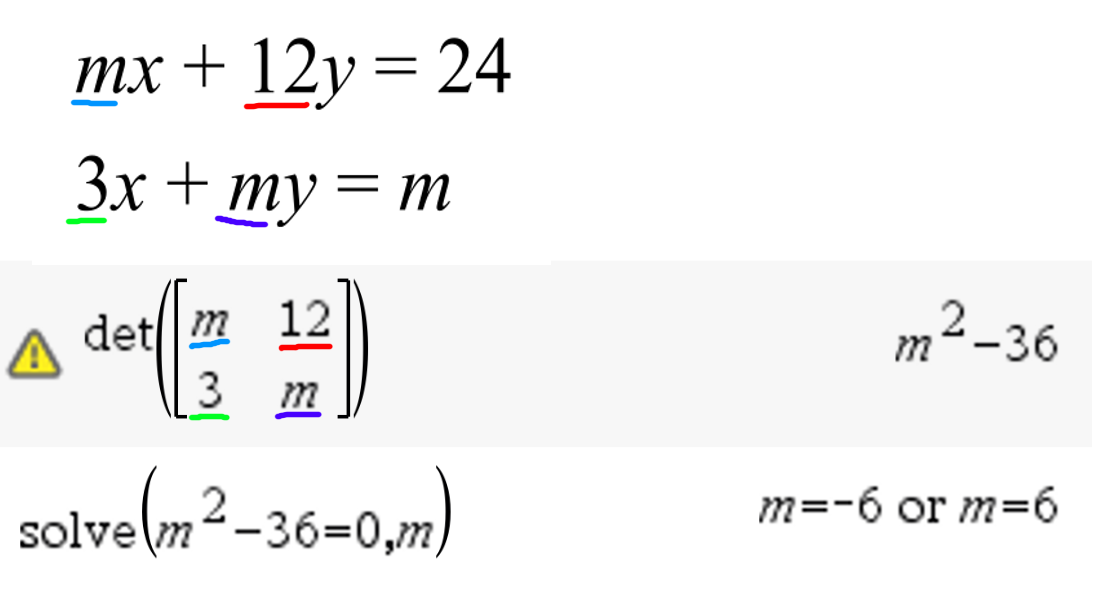
\includegraphics[width=10cm]{./img/uniquesolns.png}
			\end{examquestion}
			\begin{examquestion}{2014 VCAA Methods E2 A17}
				\begin{leftbar}
					The simultaneous linear equations $ax-3y=5$ and $3x-ay=8-a$ have no solutions for what values of $a$?
				\end{leftbar}
				Take the determinant of the 2x2 matrix of coefficients and solve for 0, then check each value it gives to see if lines are coincident or distinct parallel lines. In this case, $a=3$ produces coincidental lines, so $a=-3$ is the only solution.
			\end{examquestion}
		\subsection{Tangents}
			\begin{examquestion}{2006 VCAA Methods E2 B1}
				\begin{leftbar}
					Consider $f:[0,2\pi]\to\mathbb{R},f(x)=2\sin(x)$. The graph is shown below with tangents drawn at A and B.\\
					\begin{minipage}{0.5\linewidth}
						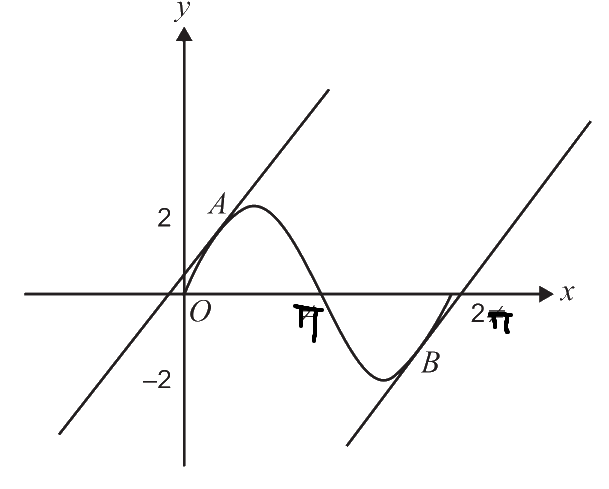
\includegraphics[width=\textwidth]{2006 E2 B1.png}
					\end{minipage}
					\hfill
					\begin{minipage}{0.5\linewidth}
						The tangent to the curve at $x=\frac{\pi}{3}$ is given by $y=x+\frac{3\sqrt{3}-\pi}{3}$.\\
						The $x$-intercept of the tangent at A is $\left(\frac{\pi-3\sqrt{3}}{3},0\right)$\\\\
						The two tangents to the curve at points A and B have gradient 1. A translation of $m$ units right in the positive $x$ direction takes the tangent at A to the tangent at B. Find $m$.
					\end{minipage}
				\end{leftbar}\mbox{}\\
				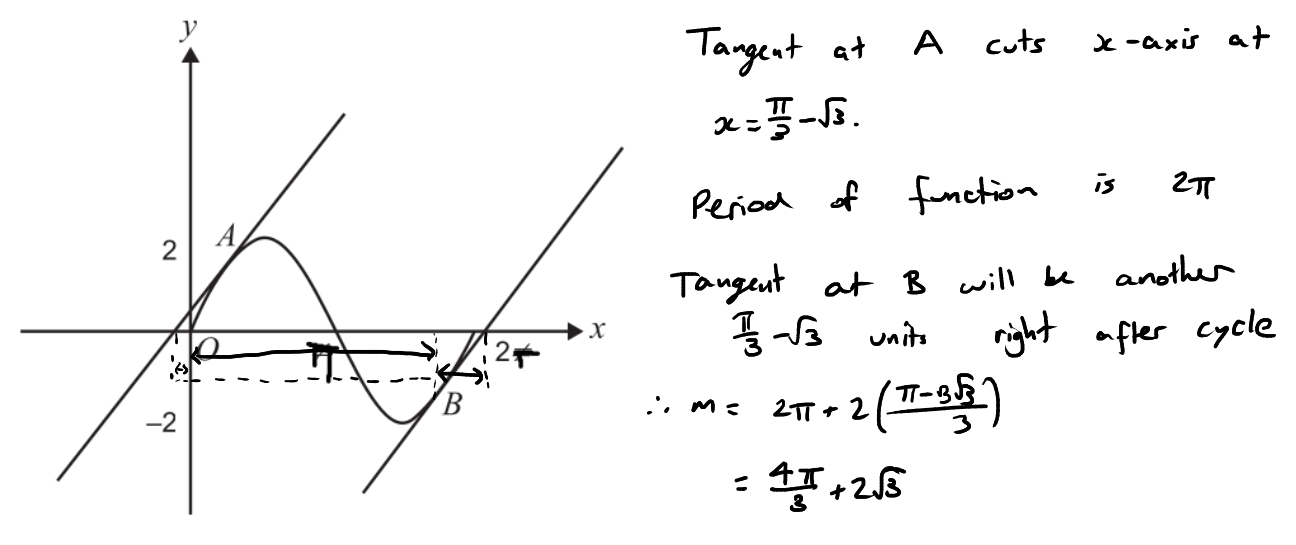
\includegraphics[width=\textwidth]{2006e2b1soln.png}
			\end{examquestion}
		\subsection{Areas}
			\begin{examquestion}{2021 NEAP Methods MCQ20}
				\begin{leftbar}
					The graph below shows a linear function $f$ and a quadratic function $g$, where $f(x)\geq g(x)$ for $x\in\R$\\
					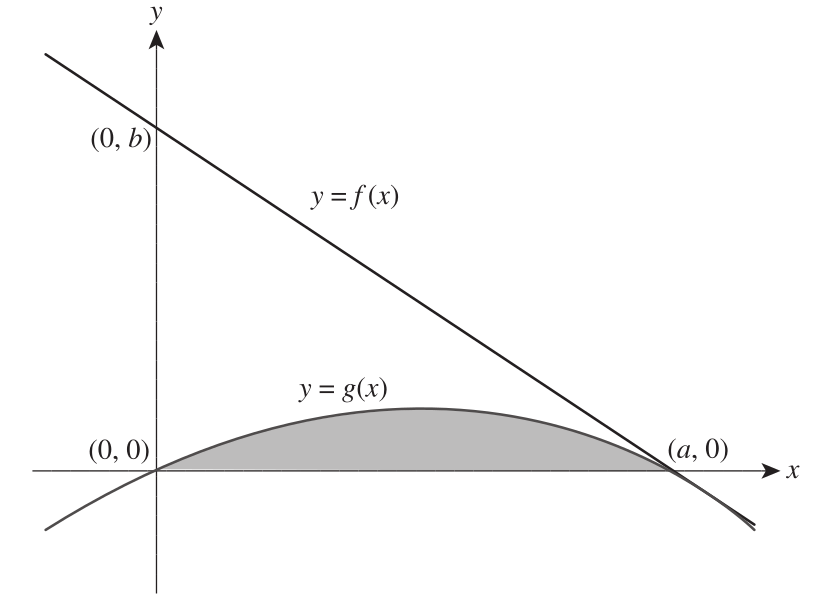
\includegraphics[width=0.5\textwidth]{2021neapmcq20.png}\\
					Given that $f(a)=g(a)$ and $f(x)=g(x)$ has one solution, the area of the shaded region in terms of $a$ and $b$ can be expressed as:
				\end{leftbar}
				Maximum area occurs when parabola is tangential to the line at $x=a$
				\begin{equation*}
					g'(x)=k(2x-a)\to g'(a)=ak
				\end{equation*}
				\begin{align*}
					m_{tangent}=-\frac{b}{a}&=g'(a)\\
					ak&=\frac{-b}{a}\\
					k&=-\frac{b}{a^2}\\\\
					\therefore g(x)&=-\frac{b}{a^2}x(x-a)\\
					\text{max area }&=\int\limits_0^a-\frac{b}{a^2}x(x-a)dx\\
					&=\frac{ab}{6}
				\end{align*}
			\end{examquestion}
	\section{Vectors and Kinematics}
		\subsection{Vectors Tech}
			\paragraph{Create a vector} ctrl+( creates a matrix which we can use for vectors.
			\subsubsection{norm(a)} Menu+7+7+1 give the norm (magnitude) of a vector.
			\subsubsection{unitV(a)} Menu+7+C+1 creates a unit vector in direction of a given vector.
			\subsubsection{dotP(a,b)} Menu+7+C+3 gives the dot product of two vectors.
			\subsubsection{crossP(a,b)} Menu+7+C+2 gives the cross product of two vectors.
			\subsubsection{sam\textunderscore vectors\textbackslash vang(a,b)} gives the angle between two vectors.
			\subsubsection{sam\textunderscore vectors\textbackslash vecres(a,b)} Put in vectors and it will find the vector resolute of $\utilde{a}$ in both the direction of and perpendicular to $\utilde{b}$.
			\subsubsection{sam\textunderscore vectors\textbackslash lindep(a,b,c,p)} Find a value for pronumeral $p$ that makes the set of vectors $a,b,c$ linearly dependent. In the first example below, we use it to find a value of p for which the vectors are linearly dependent. In the second example it is used to verify that a set of known vectors is linearly dependent. It returns a constant solution, so therefore they must be dependent.\\
			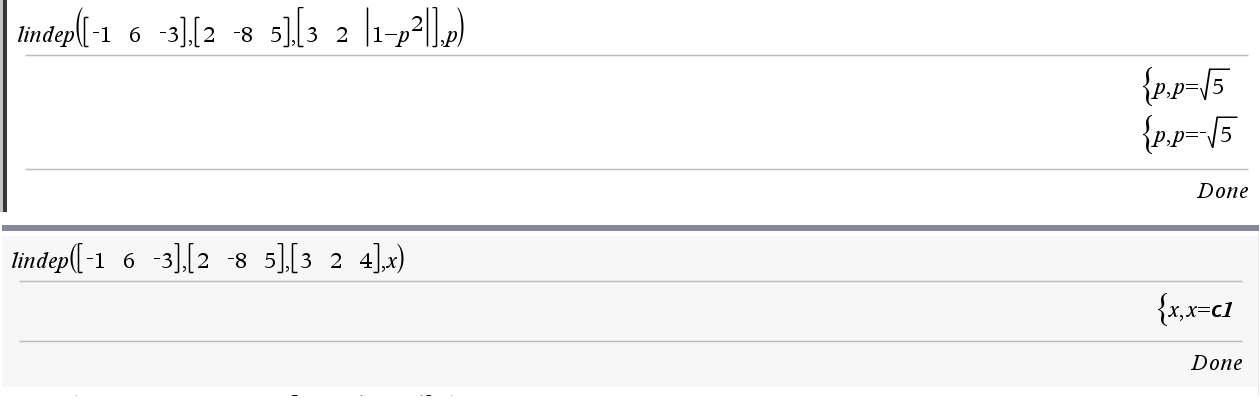
\includegraphics[width=18cm]{lindepcas.png}
		\subsection{Angles Between Vectors}
			\begin{examquestion}{2006 VCAA Spesh E2 B2}
				\begin{minipage}{\linewidth}
					\begin{leftbar}
						Point $A$ has position vector $\utilde{a}=-\utilde{i}-4\utilde{j}$, point $B$ has position vector $\utilde{b}=2\utilde{i}-5\utilde{j}$, point $C$ has position vector $\utilde{c}=5\utilde{i}-4\utilde{j}$ and point $D$ has position vector $\utilde{d}=2\utilde{i}+5\utilde{j}$. It is known that $\cos\left(\angle ADC\right)=\frac{4}{5}$. Find the cosine of $\angle ABC$ and \textbf{hence show} that $\angle ADC$ and $\angle ABC$ are supplementary (add to $\pi$).
					\end{leftbar}
				\end{minipage}
				\begin{align*}
					\overrightarrow{BA}&=-3\utilde{i}+\utilde{j} \qquad \overrightarrow{BC}=3\utilde{i}+\utilde{j}\\
					\mathrm{Let }\theta&=\angle ABC\\
					\cos\theta&=\frac{\overrightarrow{BA}\cdot\overrightarrow{BC}}{\left|\overrightarrow{BA}\right|\left|\overrightarrow{BC}\right|}\\
					&=-\frac{4}{5}\\\\
					\arccos\left(-\frac{4}{5}\right)&=\frac{\pi}{2}+\arcsin\left(\frac{4}{5}\right)\\
					\therefore \arccos\left(-\frac{4}{5}\right)+\arccos\left(\frac{4}{5}\right)&=\frac{\pi}{2}+\arcsin\left(\frac{4}{5}\right)+\arccos\left(\frac{4}{5}\right)\\
					&=\frac{\pi}{2}+\frac{\pi}{2}=\pi\\
				\end{align*}
			\end{examquestion}
		\subsection{Linear Dependence}
			\[
				x_1\utilde{a_1}+x_2\utilde{a_2}+...+x_n\utilde{a_n}=0\centernot\implies x_i=0 \forall i\in[1,n]
			\]
			A set of vectors is said to be linearly dependent if at least one of its members can be expressed as a linear combination of other vectors in the set. Alternatively, a set of vectors are linearly dependent if a vector could be removed from the set and not affect the set's span.
			\paragraph{Linear combination} A vector $\utilde{w}$ is a linear combination of $\utilde{u}$ and $\utilde{v}$ if it can be expressed in form $\utilde{w}=k_1\utilde{u}+k_2\utilde{v}$ for $k_1,k_2\in\R$.
			\paragraph{General Case} A set $S\in\R^n$ of $n$ vectors $\utilde{a}_1,\utilde{a}_2,...,\utilde{a}_n$ is linearly dependent \textbf{if and only if} there exists $k_1,k_2,...,k_n\in\R$ (not all equal 0) such that $k_1\utilde{a}_1+k_2\utilde{a}_2+...+k_n\utilde{a}_n=0$
		\subsection{Scalar Product}
			The scalar product of vectors $\utilde{a},\utilde{b}$ is given by:
			\[
			\utilde{a}\cdot\utilde{b}=|\utilde{a}||\utilde{b}|\cos\theta
			\]
			where $\theta$ is the angle between the two vectors.
			\paragraph{Properties of the Scalar Product}
			\begin{align*}
				&\utilde{a}\cdot\utilde{b}=\utilde{b}\cdot\utilde{a} &\utilde{a}\cdot\left(\utilde{b}+\utilde{c}\right)=\utilde{a}\cdot\utilde{b}+\utilde{a}\cdot\utilde{c} \\
				&k\left(\utilde{a}\cdot\utilde{b}\right)=\left(k\utilde{a}\right)\cdot\utilde{b}=a\cdot\left(k\utilde{b}\right) &\utilde{a}\cdot0=0
			\end{align*}
				\subparagraph{Parallel Vectors} For parallel vectors $\utilde{a},\utilde{b}$
				\[
					\utilde{a}\cdot\utilde{b}=\begin{cases*}
						|\utilde{a}||\utilde{b}| & if $\utilde{a},\utilde{b}$ are in the same direction \\
						-|\utilde{a}||\utilde{b}| & if $\utilde{a},\utilde{b}$ are in opposite directions
					\end{cases*}
				\]
		\subsection{Vector and Scalar Resolutes}
			We can decompose a vector $\utilde{a}$ into the sum of two vectors in perpendicular directions.
			\paragraph{Vector Resolute in General}
			The Vector resolute of $\utilde{a}$ in direction $\utilde{b}$ is given by:
			\[
				\utilde{u}=\frac{\utilde{a}\cdot\utilde{b}}{\utilde{b}\cdot\utilde{b}}\utilde{b}=\frac{\utilde{a}\cdot\utilde{b}}{|\utilde{b}|^2}\utilde{b}=\left(\utilde{a}\cdot\frac{\utilde{b}}{|\utilde{b}|}\right)\left(\frac{\utilde{b}}{|\utilde{b}|}\right)=\left(\utilde{a}\cdot\hat{\utilde{b}}\right)\hat{\utilde{b}}
			\]
			\paragraph{Scalar Resolute in General} The scalar resolute is the signed length of the vector resolute of $\utilde{a}$ in direction $\utilde{b}$
			\[
				\utilde{a}\cdot\hat{\utilde{b}}=\frac{\utilde{a}\cdot\utilde{b}}{|\utilde{b}|}
			\]
		\subsection{Vector Proofs}
			\subsubsection{Collinearity}
			Three distinct points $A, B, C$ are collinear if and only if $\overrightarrow{AC}=k\overrightarrow{AB}$ for some $k\in\R\setminus\{0\}$.
			\paragraph{Miscellaneous Facts for Proof}
				\subparagraph{Parallel Vectors} For $k\in\R^+$, the vector $k\utilde{a}$ is in the same direction as $\utilde{a}$ and has magnitude $k|\utilde{a}|$ and the vector $-k\utilde{a}$ is in the opposite direction to $\utilde{a}$ and has magnitude $k|\utilde{a}|$.\\\\
				Two non-zero vectors $\utilde{a}$ and $\utilde{b}$ are parallel if and only if $\utilde{b}=k\utilde{a}$ for some $k\in\R\setminus\{0\}$.
			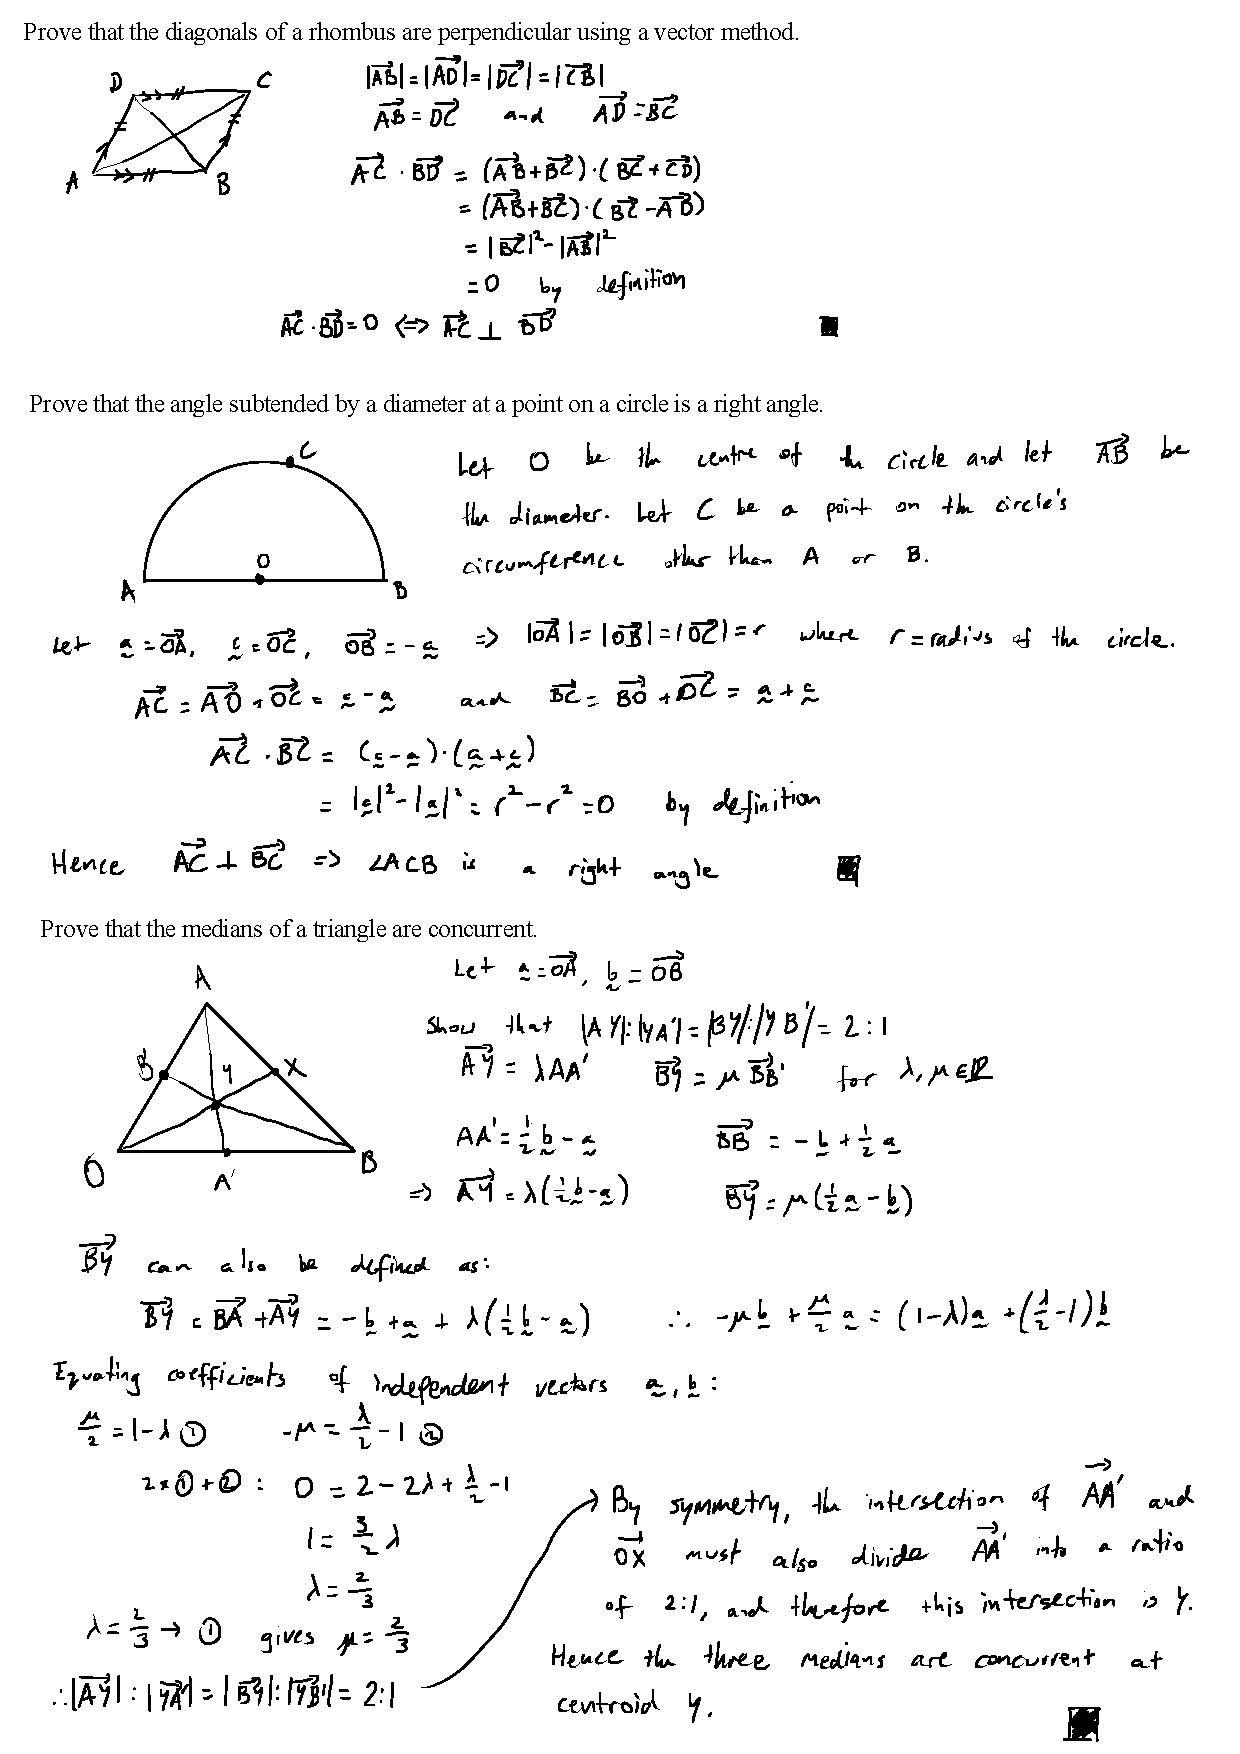
\includepdf{./pdf/vectorproofs.pdf}
		\subsection{Vector Equations}
			\paragraph{Vector Equation of Line given by Point and Direction} $\utilde{r}(\lambda)=\utilde{a}+\lambda\utilde{d},\lambda\in\R$. \textbf{Note} that there is no unique vector equation for a given line $\ell$, as we can choose any point with position vector $\utilde{a}$ as our starting point and any vector $\utilde{d}\parallel \ell$.
			
			\paragraph{Vector Equation of Line given by Two Points} $\utilde{r}(\lambda)=\utilde{a}+\lambda\left(\utilde{b}-\utilde{a}\right),\lambda\in\R$ where $\utilde{a}$ and $\utilde{b}$ are the position vectors of the two points.
			
			\paragraph{Converting from Vector to Cartesian Equation} Consider the vector equation as a set of parametrics, where the coefficient of $\utilde{i}$ is equal to $x$, coefficient of $\utilde{j}$ is equal to $y$, etc. and then solving to get the cartesian form.
			
			\paragraph{Changing from Cartesian to Vector Equation} The direction vector of the line $\utilde{d}$ is given by $\utilde{d}=\mathrm{(run)}\utilde{i}+\mathrm{(rise)}\utilde{j}$.
			
			\paragraph{Lines in 3D} Lines in three dimensions can be described in three ways, where $\utilde{a}=a_1\utilde{i}+a_2\utilde{j}+a_3\utilde{k}$ is the position vector of a point A on the line and $\utilde{d}=d_1\utilde{i}+d_2\utilde{j}+d_3\utilde{k}$ is a vector parallel to the line.
			\begin{center}
				\bgroup
				\def\arraystretch{2}
				\begin{tabularx}{\textwidth}{|m{3cm}*2{|X}|}
					\hline
					\centering Vector & Parametric & Cartesian \\
					\hline
					\vspace{2em}
					\centering$\utilde{r}(\lambda)=\utilde{a}+\lambda\utilde{d}$ & $\begin{aligned}
						x=a_1+d_2\lambda \\[1em]
						y=a_2+d_2\lambda \\[1em]
						z=a_3+d_3\lambda
					\end{aligned}$ & \(\frac{x-a_1}{d_1}=\frac{y-a_2}{d_2}=\frac{z-a_3}{d_3}\) \\
					\hline
				\end{tabularx}
				\egroup
			\end{center}
			
			\paragraph{Parallel and Perpendicular Lines} For two lines $\ell_1:\utilde{r}_1(\lambda)=\utilde{a}_1+\lambda\utilde{d}_1,\lambda\in\R$ and $\ell_2:\utilde{r}_2(\gamma)=\utilde{a}_2+\gamma\utilde{d}_2,\gamma\in\R$:
			\begin{itemize}
				\item $\ell_1\parallel\ell_2 \iff \utilde{d}_1\parallel\utilde{d}_2$
				\item $\ell_1\perp\ell_2 \iff \utilde{d}_1\perp\utilde{d}_2 \iff \utilde{d}_1\cdot\utilde{d}_2=0$
			\end{itemize}
		
			\subparagraph{Distance between two lines (non-parallel)}
			
			\subparagraph{Distance between two parallel lines} Let $\utilde{v}$ be the vector in the direction of the lines. Now let $p_1$ be a point on line 1 and $p_2$ be a point on line 2. The distance between the lines, as shown in the diagram below, can be calculated using the cross product.\\
			\begin{minipage}{0.5\linewidth}
				\begin{align*}
					d&=|\utilde{w}|\sin\theta \\
					&=\left|\utilde{\hat{v}}\times\utilde{w}\right|\\
					&=\left|\utilde{\hat{v}}\times\left(\utilde{p_2}-\utilde{p_1}\right)\right|
				\end{align*}
			\end{minipage}
			\hfill
			\begin{minipage}{0.5\linewidth}
				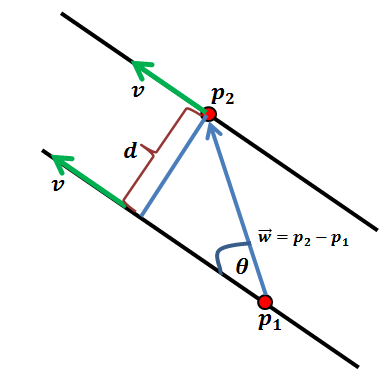
\includegraphics[width=0.5\linewidth]{vectorlinesdist.png}
			\end{minipage}
		\subsection{Intersections and Skew Lines}
			\subsubsection{Lines in 2D Space} A pair of lines in 2D space can
			\begin{itemize}
				\item intersect
				\item be parallel and distinct
				\item coincide
			\end{itemize}
			To check whether two parallel lines coincide choose a point on one line and see if it is on the other.
			
			\subsubsection{Lines in 3D Space}
				\paragraph{Skew Lines} Two lines are skew lines if they are not parallel \textbf{and} do not intersect. Two lines are skew lines \textbf{if and only if} they do not lie in the same plane.
				
				\paragraph{Coincident and Parallel Lines} We can determine whether 3D lines are coincident or parallel and distinct by similar methods as in 2 dimensions. If parallel lines share a point they must coincide.
				
				\paragraph{Intersecting Lines} Two lines $\ell_1:\utilde{r}_1(\lambda)=\utilde{a}_1+\lambda\utilde{d}_1$ and $\ell_2:\utilde{r}_2(\gamma)=\utilde{a}_2+\gamma\utilde{d}_2$ have a common point if $\exists\lambda,\gamma\in\R\ni\utilde{r}_1(\lambda)=\utilde{r}_2(\gamma)$.
				
				\paragraph{Concurrence of 3 lines} A point of concurrence is where 3 or more lines meet.
				
				\paragraph{Angle Between 2 Lines} The angle between two lines can be found using the scalar product of their direction vectors. The angle is either $\theta$ or $\pi-\theta$, whichever lies in the interval $[0,\frac{\pi}{2}]$.
		\subsection{Vector Product (Cross Product)}
			\paragraph{Geometric Relationship} The relationship between the two vectors in a cross multiplication and the result is called 'mutually perpendicular'.
			\paragraph{Properties of the Vector Product}
				\begin{itemize}
					\item Direction of $\utilde{a}\times\utilde{b}$ is perpendicular to the plane containing $\utilde{a}$ and $\utilde{b}$.
					\item $|\utilde{a}\times\utilde{b}|=|\utilde{a}||\utilde{b}|\sin\theta$
					\item $\utilde{a}\parallel\utilde{b}\implies|\utilde{a}\times\utilde{b}|=0$
					\item $\utilde{a}\perp\utilde{b}\implies|\utilde{a}\times\utilde{b}|=|\utilde{a}||\utilde{b}|$
					\item Vector product is not associative $\left(\utilde{a}\times\utilde{b}\right)\times\utilde{c}\neq\utilde{a}\times\left(\utilde{b}\times\utilde{c}\right)$
					\item Vector product is not commutative $\utilde{a}\times\utilde{b}\neq\utilde{b}\times\utilde{a}$
					\item Distributes over addition $\utilde{a}\times\left(\utilde{b}+\utilde{c}\right)=\utilde{a}\times\utilde{b}+\utilde{a}\times\utilde{c}$
					\item $\utilde{a}\times\utilde{b}=-\left(\utilde{b}\times\utilde{a}\right)$
				\end{itemize}
			
			\paragraph{Vector Product in Component Form}
				Let $\utilde{a}=a_1\utilde{\hat{i}}+a_2\utilde{\hat{j}}+a_3\utilde{\hat{k}}$ and $\utilde{b}=b_1\utilde{\hat{i}}+b_2\utilde{\hat{j}}+b_3\utilde{\hat{k}}$, then:
				\begin{align*}
					\utilde{a}\times\utilde{b}&=\left(a_1\utilde{\hat{i}}+a_2\utilde{\hat{j}}+a_3\utilde{\hat{k}}\right)\times\left(b_1\utilde{\hat{i}}+b_2\utilde{\hat{j}}+b_3\utilde{\hat{k}}\right)\\
					&=(a_2b_3-a_3b_2)\utilde{\hat{i}}-(a_1b_3-a_3b_1)\utilde{\hat{j}}+(a_1b_2-a_2b_1)\utilde{\hat{k}}
				\end{align*}
				We can also use the determinant of a $3\times3$ matrix to find the components of a vector product.
				\begin{equation*}
					\utilde{a}\times\utilde{b}=\begin{vmatrix}
						\utilde{\hat{i}} & \utilde{\hat{j}} & \utilde{\hat{k}} \\
						a_1 & a_2 & a_3 \\
						b_1 & b_2 & b_3
					\end{vmatrix}=\begin{vmatrix}
						a_2 & a_3 \\
						b_2 & b_3
					\end{vmatrix}\utilde{\hat{i}} - \begin{vmatrix}
						a_1 & a_3 \\
						b_1 & b_3
					\end{vmatrix}\utilde{\hat{j}} + \begin{vmatrix}
						a_2 & a_2 \\
						b_1 & b_2
					\end{vmatrix}\utilde{\hat{k}}
				\end{equation*}
			
			\paragraph{Area from Vector Product} $|\utilde{a}\times\utilde{b}|$ equals the area of the parallelogram spanned by $\utilde{a}$ and $\utilde{b}$
		\subsection{Vector Equations of Planes}
			\paragraph{Equations of Planes} A plane $\Pi$ can be described in 3-dimensional space with 2 vectors
			\begin{itemize}
				\item Position vector $\utilde{a}$ of a point on the plane
				\item A vector $\utilde{n}$ that is normal to the plane
			\end{itemize}
			Let $\utilde{r}$ be the position vector of a point P on the plane, then the vector $\overrightarrow{AP}=\utilde{r}-\utilde{a}$ lies on the plane and therefore $\overrightarrow{AP}\perp\utilde{n}$.\\
			\begin{align*}
				(\utilde{r}-\utilde{a})\cdot\utilde{n}&=0 \\
				\utilde{r}\cdot\utilde{n}&=\utilde{a}\cdot\utilde{n}
			\end{align*}
			The above equation is known as the \textbf{vector equation} of the plane.\\\\
			If we let $\utilde{r}=x\utilde{\hat{i}}+y\utilde{\hat{j}}+z\utilde{\hat{k}}$ and $\utilde{n}=n_1\utilde{\hat{i}}+n_2\utilde{\hat{j}}+n_3\utilde{\hat{k}}$ we can obtain the \textbf{cartesian equation} for the plane.\\
			\begin{align*}
				\utilde{r}\cdot\utilde{n}&=\utilde{a}\cdot\utilde{n} \\
				n_1x+n_2y+n_3z&=k\text{ where }k=\utilde{a}\cdot\utilde{n}
			\end{align*}
			\\\\
			We can also describe planes with the use of parameters. For example, if $n_1x+n_2y+n_3z=k$, with $a_3\neq0$ describes a plane, it can be described by the following parametrics:
			\begin{equation*}
				x=\lambda \qquad y=\gamma \qquad z=\frac{k-n_1\lambda-n_2\gamma}{n_3} \qquad \lambda,\gamma\in\R
			\end{equation*}
			We can determine the equations of planes with:
			\begin{itemize}
				\item a point on the plane and a normal vector at that point
				\item three points on the plane which are not collinear, or
				\item two lines on the plane that intersect
			\end{itemize}
		
			\begin{example}{Equation of a Plane given Point and Normal Vector}
				A plane $\Pi$ is such that the vector $-\utilde{\hat{i}}+5\utilde{\hat{j}}-3\utilde{\hat{k}}$ is normal to it at point A with the position vector $\utilde{a}=-3\utilde{\hat{i}}+4\utilde{\hat{j}}+6\utilde{\hat{k}}$ on the plane. Find the cartesian and vector equations that describe $\Pi$.\\
				\begin{align*}
					\utilde{r}\cdot\utilde{n}&=\utilde{a}\cdot\utilde{n} \\
					\utilde{r}\cdot\left(-\utilde{\hat{i}}+5\utilde{\hat{j}}-3\utilde{\hat{k}}\right)&=\left(-3\utilde{\hat{i}}+4\utilde{\hat{j}}+6\utilde{\hat{k}}\right)\cdot\left(-\utilde{\hat{i}}+5\utilde{\hat{j}}-3\utilde{\hat{k}}\right) \\
					\utilde{r}\cdot\left(-\utilde{\hat{i}}+5\utilde{\hat{j}}-3\utilde{\hat{k}}\right)&=3+20-18=5 \\
					\therefore\utilde{r}\cdot\left(-\utilde{\hat{i}}+5\utilde{\hat{j}}-3\utilde{\hat{k}}\right)&=5\\
					\\
					\\
					\utilde{r}&=x\utilde{\hat{i}}+y\utilde{\hat{j}}+z\utilde{\hat{k}} \\
					\left(x\utilde{\hat{i}}+y\utilde{\hat{j}}+z\utilde{\hat{k}}\right)\cdot\left(-\utilde{\hat{i}}+5\utilde{\hat{j}}-3\utilde{\hat{k}}\right)&=5 \\
					-x+5y-3z&=5
				\end{align*}
			\end{example}
			
			\begin{example}{Equation of Plane Given 3 Points}
				Consider the plane containing the points $A(0,1,1),B(2,1,0)$ and $C(-2,0,3)$.
				(a) Find cartesian equation of the plane.
				\begin{align*}
					\overrightarrow{AB}=2\utilde{\hat{i}}-\utilde{\hat{k}} \qquad &\text{and} \qquad \overrightarrow{AC}=-2\utilde{\hat{i}}-\utilde{\hat{j}}+2\utilde{\hat{k}} \\
					\\
					\overrightarrow{AB}\times\overrightarrow{AC}&=-\utilde{\hat{i}}-2\utilde{\hat{j}}-2\utilde{\hat{k}} \\
					\therefore \utilde{n}&=-\utilde{\hat{i}}-2\utilde{\hat{j}}-2\utilde{\hat{k}} \\
					\text{Use previous method to find plane equation to be:}\\
					-x-2y-2z&=-4
				\end{align*}
				(b) Find the axis intercepts of the plane
				\begin{align*}
					\text{x-intercept: Let }y=z=0&\implies x=4 \\ 
					\text{y-intercept: Let }x=z=0&\implies 2y=4 \implies y=2 \\
					\text{z-intercept: Let }x=y=0&\implies 2z=4 \implies z=2
				\end{align*}
			\end{example}
			
			\begin{example}{Equation of Plane Given 2 Intersecting Lines}
				Find a vector and cartesian equation of the plane containing the two lines:
				\begin{align*}
					&\ell_1: \utilde{r}_1(\lambda)=5\utilde{\hat{i}}+2\utilde{\hat{j}}+\lambda\left(2\utilde{\hat{i}}+\utilde{\hat{j}}+\utilde{\hat{k}}\right) \qquad \text{and} \\ &
					\ell_2: \utilde{r}_2(\gamma)=-3\utilde{\hat{i}}+4\utilde{\hat{j}}+6\utilde{\hat{k}}+\gamma\left(\utilde{\hat{i}}-\utilde{\hat{j}}-2\utilde{\hat{k}}\right)
				\end{align*}
				\begin{align*}
					\utilde{a}&=5\utilde{\hat{i}}+2\utilde{\hat{j}}\text{ is on the plane} \\
					\\
					\text{Let $\utilde{n}$ be the a vector perpendicular to both } & \text{$\utilde{d}_1$ and $\utilde{d}_2$} \\
					\utilde{n}&=\utilde{d}_2\times\utilde{d}_2 \\
					&=-\utilde{\hat{i}}+5\utilde{\hat{j}}-3\utilde{\hat{k}} \\
					\\
					\therefore \utilde{r}\cdot\left(-\utilde{\hat{i}}+5\utilde{\hat{j}}-3\utilde{\hat{k}}\right)&=\utilde{a}\cdot\utilde{n}\\
					&=-1\times5+2\times5+-3\times0 \\
					\therefore\utilde{r}\cdot\left(-\utilde{\hat{i}}+5\utilde{\hat{j}}-3\utilde{\hat{k}}\right)&=5 \\
					\implies -x+5y-3z=5
				\end{align*}
			\end{example}
		\subsection{Distances, Angles, Intersections of Planes}
			\subsubsection{Distances}
				\paragraph{Point to Plane distance} The distance from a point $P$ to a plane $\Pi$ is given by
				\[
					d=\left|\overrightarrow{PQ}\cdot\utilde{\hat{n}}\right|
				\]
				where $Q$ is any point on the plane and $\hat{n}$ is a unit vector normal to the plane
				
				\paragraph{Plane to Origin Distance} A plane that does not pass through the origin has a vector equation $\utilde{r}\cdot\utilde{n}=k$ for $k\neq0$. Take the point $M$ as the closest point on the plane to the origin. $\overrightarrow{OM}=m\utilde{n}$ where $|m|$ is the distance of the plane to the origin.
				\begin{align*}
					&\left(m\utilde{\hat{n}}\right)\cdot\utilde{n}=k \\
					&m\left(\utilde{\hat{n}}\cdot\utilde{n}\right)=m|\utilde{n}|=k\\
					&\therefore m=\frac{k}{|\utilde{n}|}
				\end{align*}
			
				\paragraph{Distance Between Parallel Planes} To find the distance between planes $\Pi_1$ and $\Pi_2$ we choose any point $P$ on $\Pi_1$ and find its nearest distance to $\Pi_2$, we can also use each plane's distance from origin.
				\begin{example}{Distance Between Parallel Planes}
					\begin{leftbar}
						Consider the planes given by:
						\[
							\Pi_1:2x-y+2z=5\qquad\Pi_2:2x-y+2z=-2
						\]
						Find the distance between the two planes.
					\end{leftbar}\mbox{}\\
					First, we find the distance of each plane from the origin.\\
					\begin{align*}
						\utilde{n}&=2\utilde{i}-\utilde{j}+2\utilde{k}\implies |\utilde{n}|=3\\\\
						\text{Signed distance from origin of }\Pi_1&=\frac{5}{|\utilde{n}|}=\frac{5}{3}\\
						\text{Signed distance from origin of }\Pi_2&=\frac{-2}{|\utilde{n}|}=\frac{-2}{3}\\
						\therefore\text{Distance between planes}&=\frac{5}{3}-\left(\frac{-2}{3}\right)\\
						&=\frac{7}{3}
					\end{align*}
				\end{example}
				
				\paragraph{Distance Between Skew Lines} Given two skew lines it can be shown that there is a unique line segment $PQ$ joining them that is perpendicular to both lines. Consider the lines defined by $\utilde{r}_1(\lambda)=\utilde{a}_1+\lambda\utilde{d}_1,\lambda\in\R$ and $\utilde{r}_2(\gamma)=\utilde{a}_2+\gamma\utilde{d}_2,\gamma\in\R$. The distance between these skew lines is given by:
				\[
					d=\left|\left(\utilde{a}_2-\utilde{a}_1\right)\cdot\utilde{\hat{n}}\right|\qquad \hat{\utilde{n}}=\frac{\utilde{d}_1\times\utilde{d}_2}{|\utilde{d}_1\times\utilde{d}_2|}
				\]
				\begin{examquestion}{2023 MAV Spec E2 QB2d}
					\begin{leftbar}
						Determine the shortest distance between the skew lines:
						\begin{equation*}
							l_1: \utilde{r}_1(\lambda)=(3+3\lambda)\utilde{i}+(2-3\lambda)\utilde{j}+(2\lambda-1)\utilde{k},\lambda\in\R\qquad l_2: \frac{x-4}{7}=\frac{y+1}{13}=\frac{z-5}{9}
						\end{equation*}
						Let $\utilde{n}$ be a vector perpendicular to both lines.
						\[
							\utilde{n}=\left(7\utilde{i}+13\utilde{j}+9\utilde{k}\right)\times\left(3\utilde{i}-3\utilde{j}+2\utilde{k}\right)=53\utilde{i}+13\utilde{j}-60\utilde{k}
						\]
						A(3,2,-1) lies on $l_1$ and $P(4,-1,5)$ lies on $l_2$. Therefore $\overrightarrow{AP}=\utilde{i}-3\utilde{j}+6\utilde{k}$. The distance between the lines is $\left|\overrightarrow{AP}\cdot\hat{\utilde{n}}\right|=4.27$
					\end{leftbar}
				\end{examquestion}
			
			\subsubsection{Intersections and Angles}
				Two planes that are not parallel will intersect along a line. To find the angle between the planes choose a point $P$ common to both planes and find the angle $\theta$ between the normal vectors. The answer will either be $\theta$ or $\pi-\theta$, whichever is in the interval $[0,\frac{\pi}{2}]$.
				
				\paragraph{Intersection of a Line and a Plane} The angle between a line and a plane is 90\degree-$\theta$ where $\theta$ is the angle between the line and a normal to the plane. To find the point of intersection between a plane and line, we need to find a value for $t$ for which $\utilde{r}(t)$ represents a point on the line. That is, $\utilde{r}(t)\cdot\utilde{n}=k$. This will help us find a $t$ value and then by subbing back in we find the point of intersection.
				\begin{example}{Intersection of Line and Plane}
					\begin{leftbar}
						Consider the line represented by $\utilde{r}(\lambda)=3\utilde{i}-\utilde{j}-\utilde{k}+\lambda(\utilde{i}+2\utilde{j}-\utilde{k})$ and the plane represented by $\utilde{r}\cdot(\utilde{i}+\utilde{j}+2\utilde{k})=2$. Find the point of intersection and angle of intersection between the line and plane.
					\end{leftbar}
					\begin{minipage}[t]{0.5\linewidth}
						\underline{Point of Intersection}\\
						\begin{align*}
							\utilde{r}(\lambda)\cdot(\utilde{i}+\utilde{j}+2\utilde{k})&=2\\
							\left(3\utilde{i}-\utilde{j}-\utilde{k}+\lambda\left(\utilde{i}+2\utilde{j}-\utilde{k}\right)\right)\cdot(\utilde{i}+\utilde{j}+2\utilde{k})&=2\\
							(3+\lambda)+(-1+2\lambda)+2(-1-\lambda)&=2\\
							\therefore \lambda&=2\\
							\utilde{r}(2)=5\utilde{i}+3\utilde{j}-3\utilde{k}&
						\end{align*}
						Therefore the point of intersection is (5,3,-3).
					\end{minipage}
					\hfill
					\begin{minipage}[t]{0.5\linewidth}
						\underline{Angle of Intersection}\\
						$\utilde{d}=\utilde{i}+2\utilde{j}-\utilde{k}$ is parallel to the line and $\utilde{n}=\utilde{i}+\utilde{j}+2\utilde{k}$ is normal to the plane.
						\begin{align*}
							\utilde{d}\cdot\utilde{n}&=|\utilde{d}||\utilde{n}|\cos\theta\\
							1&=6\cos\theta\\
							\theta&=80.4\degree
						\end{align*}
						Therefore the angle of intersection is $90\degree-80.4\degree$ as $80.4\degree$ is the angle with the normal. Hence the angle of intersection is $9.6\degree$.
					\end{minipage}
				\end{example}
			
			\subsubsection{Intersection of Planes}
				\begin{example}{Equation of the Line of Intersection}
					\begin{leftbar}
						Let $\Pi_1$ and $\Pi_2$ be planes represented by:
						\[
							\Pi_1:\utilde{r}\cdot(\utilde{i}+\utilde{j}-3\utilde{k})=6\qquad\Pi_2:\utilde{r}\cdot(2\utilde{i}-\utilde{j}+\utilde{k})=4
						\]
						Find a vector equation to describe the line of intersection of these planes.
					\end{leftbar}
					Consider the cartesian equations of two planes:
					\begin{align*}
						x+y-3z=6\quad(1)\qquad&\qquad2x-y+z=4\quad(2)\\
						(1)+(2)\rightarrow3x-2z&=10\quad(3)\\
						\text{Let }x=\lambda\implies z=\frac{3\lambda-10}{2} &\text{ (from (3)) },y=\frac{7\lambda-18}{2} \text{ (from (2))}\\
						\text{This gives us the parametric equations for the line of intersection:}\\
						x=\lambda,&y=\frac{7\lambda-18}{2},z=\frac{3\lambda-10}{2}\\
						\text{Converting to vector form:}\\
						\utilde{r}(\lambda)=-9\utilde{j}-5\utilde{k}+\lambda\left(\utilde{i}+\frac{7}{2}\utilde{j}+\frac{3}{2}\utilde{k}\right)
					\end{align*}
				\end{example}
				\begin{examquestion}{2023 MAV Spec E2 QBcii}
					\begin{leftbar}
						Find a Cartesian equation for the line $l_2$ contained in both $\Pi_1$ and $\Pi_2$ where
						\[
							\Pi_1: 3x-3y+2z=25 \qquad \Pi_2: 2x+y-3z=-8
						\]
					\end{leftbar}
					The line contained in both $\Pi_1$ and $\Pi_2$ is perpendicular to the normals of both planes. That, is $l_2$ is parallel to:
					\[
						\left(3\utilde{i}-3\utilde{j}+2\utilde{k}\right)\times\left(2\utilde{i}+\utilde{j}-3\utilde{k}\right)=7\utilde{i}+13\utilde{j}+9\utilde{k}
					\]
					The line has to pass through point $P(4,-1,5)$ on $\Pi_2$ (given in previous part), therefore the vector equation of $l_2$ is:
					\[
						\utilde{r}(\lambda)=4\utilde{i}-\utilde{j}+5\utilde{k}+\lambda\left(7\utilde{i}+13\utilde{j}+9\utilde{k}\right)
					\]
					By looking at \textbf{Lines in 3D} in Section 5.7, we can see that:
					\begin{align*}
						&a_1=4\quad a_2=-1\quad a_3=5 \quad d_1=7\quad d_2=13\quad d_3=9\\
						&\implies \frac{x-4}{7}=\frac{y+1}{13}=\frac{z-5}{9}
					\end{align*}
				\end{examquestion}
			
		\subsection{Parametric Vector Equations}
			
		\subsection{SUVAT and Constant Acceleration}
			\[
				v=u+at \qquad s=ut+\frac{1}{2}at^2 \qquad v^2=u^2+2as \qquad s=\frac{1}{2}(u+v)t
			\]
		
		\subsection{Terminal (Limiting) Velocity}
			\begin{examquestion}{VCAA 2017 Spesh E2 B2c}
				\begin{leftbar}
					After two seconds of falling, a skydiver's acceleration is affected by air resistance such that their acceleration is given by:
					\[
						a=g-0.01v^2
					\]
					Find the limiting (terminal) velocity in $m s^{-1}$ that they would reach.
				\end{leftbar}
				\begin{align*}
					\text{Let }a&=0\\
					g&=0.01v^2\\
					v&=10\sqrt{g}
				\end{align*}
			\end{examquestion}
		\subsection{Velocity Functions of Time}
			\begin{examquestion}{VCAA 2007 Spesh E2 B5}
				\begin{leftbar}
					A car travelling at $20 m s^{-1}$ passes a stationary police car, and then decelerates so that its velocity $v m s^{-1}$, at time $t$ seconds after passing the police car, is given by $v=20-2\arctan(t)$.\\
					b) Explain why $v$ will never equal 16.\\
					\begin{align*}
						t&\to\infty,\arctan(t)\to\frac{\pi}{2}\\
						v&\to\left(20-2\cdot\frac{\pi}{2}\right)^+=(20-\pi)^+\\
						v&>20-\pi>16
					\end{align*}
				\end{leftbar}
			\end{examquestion}
		\subsection{Velocity-Time Graphs}
			\paragraph{Displacement} is given by the signed area bounded by the graph and the $t$-axis.
			\paragraph{Acceleration} is given by the gradient.
			\paragraph{Distance} is given by the total area bounded by the graph and the $t$-axis.
		\subsection{Vector Functions}
			\subsubsection{Describing Particle's Path}
				Consider $\utilde{r}(\lambda)=x(\lambda)\utilde{i}+y(\lambda)\utilde{j},\lambda\in\R$. $\utilde{r}(\lambda)$ represents a family of vectors defined by the parameter $\lambda$. Solve the components as normal parametrics to obtain the equation of the path.
			\subsubsection{Describing Curves with Vector Functions}
				Vector functions to describe curves are not unique.
		\subsection{Position Vectors as a Function of Time}
			Consider the vector function $\utilde{r}(t)=\cos(t)\utilde{i}+\sin(t)\utilde{j},t\geq0$.
			\begin{itemize}
				\item At $t=0$, $\utilde{r}(t)=\utilde{i}$ so the particle starts at $(1,0)$
				\item The particle moves at a constant speed along $x^2+y^2=1$
				\item The particle moves counterclockwise (sub in successive $t$ values)
				\item The period of the motion is $2\pi$; it takes $2\pi$ units of time to complete one circle.
			\end{itemize}
			\begin{examquestion}{2019 MAV Spesh E2 QA13}
				\begin{leftbar}
					John is riding a jet ski. The ski is level with the pier (origin) and is travelling $5m s^{-1}$ due North when John decides to accelerate uniformly. After accelerating for 40 seconds he is now travelling due East at $4m s^{-1}$. Given the unit vectors $\utilde{i}$ and $\utilde{j}$ are directed East and North respectively, find the position of the jet ski after the 40 second time period.
				\end{leftbar}
				\begin{align*}
					\utilde{a}&=\frac{4\utilde{i}-\utilde{5}j}{40}\\
					\utilde{r}&=5\utilde{i}\times40+\frac{1}{2}\left(\frac{4\utilde{i}-\utilde{5}j}{40}\right)\times40^2 \text{(Constant acceleration formula as acceleration is uniform)}\\
					&=80\utilde{i}+100\utilde{j}
				\end{align*}
			\end{examquestion}
		\subsection{Vector Calculus}
			\subsubsection{Properties of Vector Derivatives}
				\begin{align*}
					&\frac{d}{dt}\left(\utilde{c}\right)=0 \qquad \text{For constant vector }\utilde{c} \qquad &\frac{d}{dt}\left(k\utilde{r}(t)\right)=k\frac{d}{dt}\left(\utilde{r}(t)\right),k\in\R\\
					&\frac{d}{dt}\left(\utilde{r}_1(t)+\utilde{r}_2(t)\right)=\frac{d}{dt}\left(\utilde{r}_1(t)\right)+\frac{d}{dt}\left(\utilde{r}_2(t)\right) \qquad &\frac{d}{dt}\left(f(t)\cdot\utilde{r}(t)\right)=f(t)\frac{d}{dt}\left(\utilde{r}(t)\right)+\utilde{r}(t)\frac{d}{dt}\left(f(t)\right),f:\mathbb{D}\to\R\\
				\end{align*}
			\subsubsection{Vector Antidifferentiation}
				Consider:
				\[
					\int\utilde{r}(\lambda)d\lambda=\int x(\lambda)\utilde{i}+y(\lambda)\utilde{j}+z(\lambda)\utilde{k}d\lambda=\left(\int x(\lambda)d\lambda\right)\utilde{i}+\left(\int y(\lambda)d\lambda\right)\utilde{j}+\left(\int z(\lambda)d\lambda\right)\utilde{k}=X(\lambda)\utilde{i}+Y(\lambda)\utilde{j}+Z(\lambda)\utilde{k}+\utilde{c},\utilde{c}\in\R^3
				\]
				Where $\frac{dX}{d\lambda}=x(\lambda)$ and $\frac{dY}{d\lambda}=y(\lambda)$ and $\frac{dZ}{d\lambda}=z(\lambda)$ and $\utilde{c}$ is a constant vector.
			\subsubsection{Velocity and Acceleration Along a Curve}
				Consider a particle with position vector $\utilde{r}(t)=x(t)\utilde{i}+y(t)\utilde{j}$.
				\paragraph{Velocity} $\utilde{v}=\utilde{\dot{r}}(t)=\dot{x}(t)\utilde{i}+\dot{y}(t)\utilde{j}$
				\paragraph{Acceleration} $\utilde{a}(t)=\utilde{\ddot{r}}(t)=\ddot{x}(t)\utilde{i}+\ddot{y}(t)\utilde{j}$
				\paragraph{Distance Between Points on Vector Function Curve} $|\utilde{r}(t_1)-\utilde{r}(t_0)|$
				\paragraph{Distance traversed along the curve} If $\utilde{r}(\lambda)=x(\lambda)\utilde{i}+y(\lambda)\utilde{j}$ describes the path of a particle, the distance traversed along the curve from $\lambda=a$ to $\lambda=b$ is given by:
				\[
					\int\limits_a^b\sqrt{\left(\frac{dx}{d\lambda}\right)^2+\left(\frac{dy}{d\lambda}\right)^2}d\lambda
				\]
			\subsubsection{Alternative Forms of Acceleration}
			\[
				a=\frac{d^2x}{dt^2}=\frac{dv}{dt}=v\frac{dv}{dx}=\frac{d}{dx}\left(\frac{1}{2}v^2\right)
			\]
			\begin{examquestion}{2015 MAV Spesh E2 A18}
				\begin{leftbar}
					A body moves in a straight line such that its velocity is given by $v=(1-x)^2$ where $x$ is the displacement from the origin. If the body starts at the origin, its acceleration after 2 seconds is?
				\end{leftbar}
				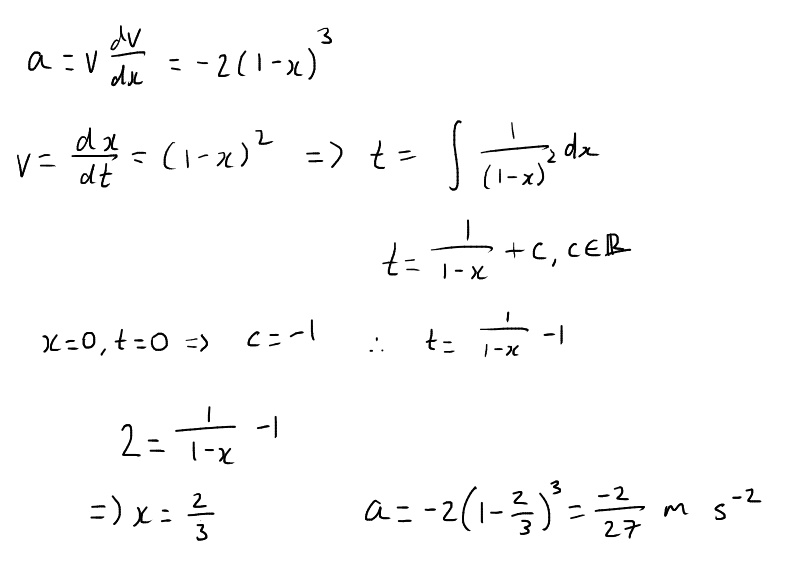
\includegraphics[width=\textwidth]{./img/2015mave2a18.png}
			\end{examquestion}
	\section{Complex Numbers}
		\subsection{Tech}
			\subsubsection{Lines in the Complex Plane} Define z:=x+y$\cdot\mathbf{i}$, then Menu+3+1 to get the solve() function and then input your complex relation, and solve for $y$.
			
			\subsubsection{Relations with Arguments in the Complex Plane} For relations in form $\Arg(z)=a$ we define z:=x+y$\cdot\mathbf{i}$, and then use Menu+2+9+4 to input the angle() function. We then menu+3+1 solve(angle(z)=a,y) to get the relation.
		\subsection{Operations of Complex Numbers in Cartesian Form}
			For $z_1=a+bi$ and $z_2=c+di$ for $a,b,c,d\in\R$
			\begin{align*}
				z_1+z_2=(a+c)+(b+d)i \qquad z_1z_2=(ac-bd)+(ad+bc)i \\
				z_1-z_2=(a-c)+(b-d)i \qquad kz=ka+kbi
			\end{align*}
			\begin{minipage}{0.5\textwidth}
				\paragraph{Multiplication by i} $z\times i,z\in\mathbb{C}$ gives a $\frac{\pi}{2}$ rotation in the counterclockwise direction about the origin.
				\begin{align*}
					i^{4n}=1 \qquad i^{4n+1}=i \qquad i^{4n+2}=-1 \qquad i^{4n+3}=-i
				\end{align*}
			\end{minipage}
			\hfill
			\begin{minipage}{0.4\textwidth}
				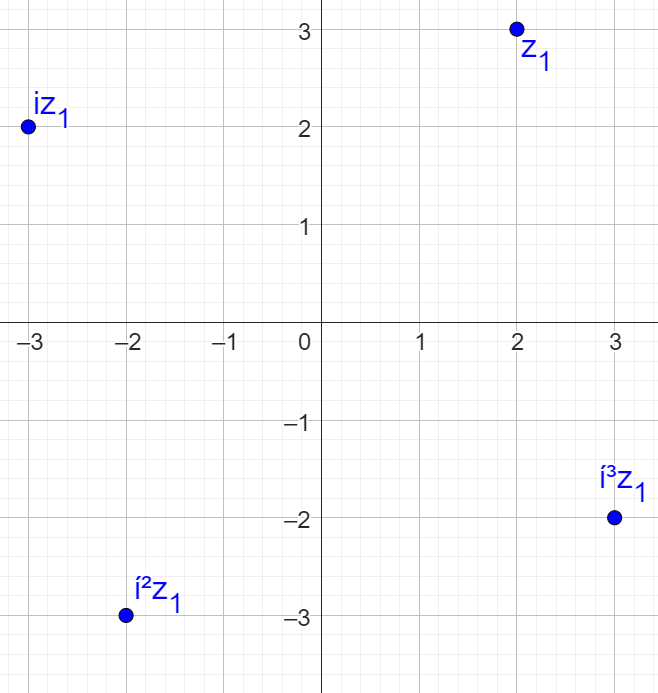
\includegraphics[width=\linewidth]{argandrotate.png}
			\end{minipage}
			\begin{examquestion}{2012 VCAA Spesh E2 QA6}
				\begin{leftbar}
					For any complex number $z$, the location on an Argand diagram of the complex number $i^3\bar{z}$ can be found by:\\
					A) Rotating $z$ through $\frac{3\pi}{2}$ counterclockwise about origin.\\
					B) Reflecting $z$ about the $x$-axis and then reflecting about the $y$-axis.\\
					C) Reflecting $z$ about the $y$-axis and then rotating anticlockwise through $\frac{\pi}{2}$ about the origin.\\
					D) Reflecting $z$ about the $x$-axis and then rotating anticlockwise through $\frac{\pi}{2}$ about the origin.\\
				\end{leftbar}
				$i^3\bar{z}$ is a reflection of $z$ in the $x$-axis followed by a $\frac{3\pi}{2}$ rotation anticlockwise about the origin. The result is the same as C.
			\end{examquestion}
		\subsection{Properties of Conjugates}
			For $z=a+bi$, $\bar{z}=a-bi$
			\[
				\bar{z_1+z_2}=\bar{z_1}+\bar{z_2} \qquad \bar{z_1z_2}=\bar{z_1}\bar{z_2} \qquad \bar{kz}=k\bar{z},k\in\R \qquad z\bar{z}=|z|^2 \qquad z+\bar{z}=2\Re(z)
			\]
			\paragraph{Multiplicative Inverse for Division} If $z=a+bi\neq0$ then
			\[
				z^{-1}=\frac{a-bi}{a^2+b^2}=\frac{\bar{z}}{|z|^2}
			\]
			For division:
			\[
				\frac{z_1}{z_2}=z_1z_2^{-1}=\frac{z_1\bar{z_2}}{|z_2|^2}
			\]
		\subsection{Polar Form Operations}
			\paragraph{Conjugate} $z=r\cis\theta\implies\bar{z}=r\cis\left(-\theta\right)$. On an Argand diagram this can be represented as a reflection of $z$ in the Real axis.
			\paragraph{Addition and Subtraction} You need to convert to cartesian form to complete these operations using $\cis\theta=(\cos\theta+i\sin\theta)$.
			\paragraph{Scalar Multiplication} If $k\in\R^+$ then $\Arg(z)=Arg(kz)$. If $k\in\R^-$ then:
			\[
				\Arg(kz)=\begin{cases*}
					\Arg(z)-\pi & $0<\Arg(z)\leq\pi$ \\
					\Arg(z)+\pi & $-\pi<\Arg(z)\leq0$
				\end{cases*}
			\]
			\paragraph{Complex Multiplication} Let $z_1=r_1\cis\theta_1$ and $z_2=r_2\cis\theta_2$
			\[
				z_1z_2=r_1r_2\cis(\theta_1+\theta_2) \qquad \Arg(z_1z_2)=\Arg(z_1)+\Arg(z_2)+2k\pi,k\in\{-1,0,1\}
			\]
			\paragraph{Complex Division} Let $z_1=r_1\cis\theta_1$ and $z_2=r_2\cis\theta_2$, $r_2\neq0$.
			\[
				\frac{z_1}{z_2}=\frac{r_1}{r_2}\cis\left(\theta_1-\theta_2\right) \qquad \Arg(z_1z_2)=\Arg(z_1)-\Arg(z_2)+2k\pi,k\in\{-1,0,1\}
			\]
			$\Arg(\frac{1}{z})=-\Arg(z)$ given $z\notin\R^-$
		\subsection{Quadratics over Complex Numbers}
			\paragraph{Sum of Squares} Since $i^2=-1$, we can rewrite a sum of squares as a difference of squares using $i$. $z^2+a^2=z^2-(ai)^2=(z+ai)(z-ai)$
		\subsection{Polynomials over Complex Numbers}
			\paragraph{Remainder Theorem} Let $\alpha\in\mathbb{C}$. When a polynomial $P(z)$ is divided by $z-\alpha$, the remainder is $P(\alpha)$
			\paragraph{Factor Theorem} Let $\alpha\in\mathbb{C}$. Then $z-\alpha$ is a factor of $P(z)$ \textbf{if and only if} $P(a)=0$.
			\paragraph{Conjugate Root Theorem} Let $P(z)$ be a polynomial with real coefficients. If $a+bi$ is a solution to $P(z)=0$, with $a,b\in\R$, then the complex conjugate $a-bi$ is also a solution.
			\paragraph{The Fundamental Theorem of Algebra} Every polynomial $P(z)=a_nz^n+a_{n-1}z^{n-1}+...+a_1z+a_0$ of degree $n$, where $n\geq1$ and the coefficients $a_i$ are complex numbers, has at least one linear factor in the complex number system.
			\begin{examquestion}{VCAA 2007 Spesh E2 A6}
				\begin{leftbar}
					Which one of the following diagrams would represent the roots of $z^5,z^2-z+c=0$ in the complex plane for $z\in\mathbb{C}$ and $c\in\R$?
					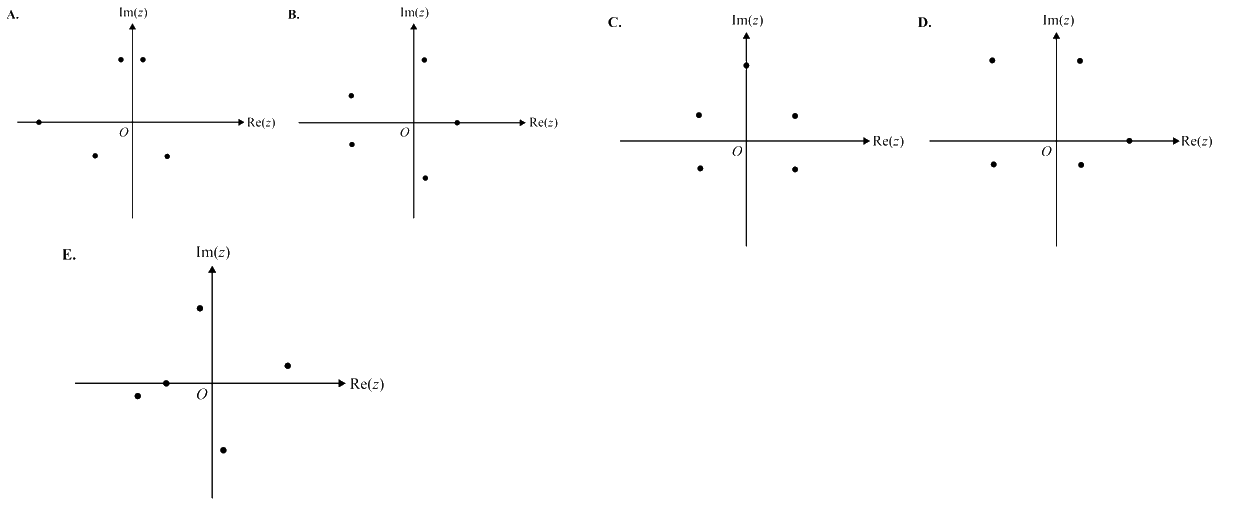
\includegraphics[width=\linewidth]{2007e2a6.png}
				\end{leftbar}
				As the coefficients of $z$ are all real numbers, therefore the roots will exist in conjugate pairs. Thus it is \textbf{B}.
			\end{examquestion}
		\subsection{Solving with De Moivre}
			Equations of form $z^n=a,a\in\mathbb{C}$ can be solved with de Moivre's theorem.
			\begin{example}{de Moivre's theorem to solve basic case}
				Let $z=r\cis\theta$ and $a=q\cis\phi$. Solve $z^n=a$.
				\begin{align*}
					&z=r\cis\theta,a=q\cis\phi &\cis(n\theta)=\cis\phi\\
					&z^n=a &n\theta=\phi+2k\pi,k\in\mathbb{Z}\\
					&r^n\cis(n\theta)=q\cis\phi &\theta=\frac{1}{n} (\phi+2k\pi),k\in\mathbb{Z}\\
					&r=\sqrt[n]{q}\\
				\end{align*}
				We then use the information to begin finding solutions.
			\end{example}
		
			\paragraph{Complex Roots}
			\begin{itemize}
				\item For $n\in\mathbb{N}$ and $a\in\mathbb{C}$, the solutions $z^n=a$ are called the nth-roots of $a$
				\item Solutions lie evenly spaced on a circle about the origin of radius $|a|^{\frac{1}{n}}$.
				\item There are n solutions and they are spaced equally around the circle by intervals of $\frac{2\pi}{n}$
			\end{itemize}
			
			\paragraph{Roots of Unity} For $n\in\mathbb{N}$ the solutions of $z^n=1$ are called the nth-roots of unity.
			\begin{itemize}
				\item Solutions lie on the unit circle
				\item There are n solutions and they are spaced evenly by $\frac{2\pi}{n}$ around the circle
				\item $z=1$ is always a solution
			\end{itemize}
		
			\paragraph{Sum of the nth-roots of Unity} $z^n=1$ has a set of solutions defined by the geometric sequence with ratio $w=\cis\left(\frac{2\pi}{n}\right)$. The sum of the nth-roots of unity is always 0.
			\[
				1,w,w^2,w^3,w^4,...,w^{n-1},w=\cis\left(\frac{2\pi}{n}\right),n\in\mathbb{N}
			\]
			\[
				\sum\limits_{i=0}^{n-1}w^i=0 \text{ For }w=\cis\left(\frac{2\pi}{n}\right),w^n=1
			\]
		\subsection{Subsets of Complex Plane}
			\subsubsection{Circles}
				A circle is defined as the set of points equidistant from a complex number.\\
				For $z,z_1\in\mathbb{C}$ we can form a circle of radius $r$ about $z_1$ by:
				\[
					\left(z-z_1\right)\overline{\left(z-z_1\right)}=r^2\implies |z-z_1|^2=r^2 \implies |z-z_1|=r
				\]
				\paragraph{Combination of Moduli} As $|z|=|\bar{z}|$, a linear combination of the moduli $a|z|+b|\bar{z}|=r(a+b)$ will be a circle of radius $r$.
				\paragraph{Find Equation of Circle given Endpoints of Diameter} If $z_1$ and $z_2$ are the endpoints of the diameter of a circle, then the equation of a circle can be determined in \textbf{diametric form}:
				\[
					(z-z_1)\overline{\left(z-z_2\right)}+(z-z_2)\overline{\left(z-z_1\right)}=0
				\]
				\paragraph{Equation from Three Points} Given three complex numbers that lie on a circle, the centre $z_0$ can be found by finding the intersection of the perpendicular bisectors of the points.
				\[
					r=|z_0-z_1|=|z_0-z_2|=|z_0-z_3|\qquad z,z_1,z_2,z_3\in\mathbb{C}
				\]
			\subsubsection{Lines}
				\paragraph{Perpendicular Bisectors} The set of points equidistant on the complex plane from two complex numbers form a line.
				\[
					|z-z_1|=|z-z_2|\qquad z,z_1,z_2\in\mathbb{C}
				\]
					\subparagraph{Converting Perpendicular Bisector to Cartesian Form} First find midpoint of the line between $z_1$ and $z_2$. Determine the slope between the points and take its negative reciprocal. Substitute in to $y=m(x-x_1)+y_1$.
				\begin{examquestion}{VCAA Spesh 2017 E2 B4f}
					\begin{leftbar}
						The equation of the line passing through the two roots of $z^2+4z+16=0,z\in\mathbb{C}$ can be expressed as $|z-a|=|z-b|$. Find $b$ in terms of $a$.
					\end{leftbar}
					\begin{align*}
						\text{Let }a=\Re(a)+\Im(a)i&\qquad b=\Re(b)+\Im(b)i\\
						\frac{\Re(a)+\Re(b)}{2}=-2&\qquad\Im(b)=\Im(a)\\
						\implies \frac{a+b}{2}&=-2+\Im(a)i\\
						\therefore b=-4-a+2\Im(a)i&=-4-(\Re(a)+\Im(a)i)+2\Im(a)i=-4-\Re(a)-\Im(a)i+2\Im(a)i\\
						\therefore b&=-4-(\Re(a)-\Im(a)i)=-4-\bar{a}
					\end{align*}
				\end{examquestion}
			\subsubsection{Rays}
				A ray extending at angle $\theta$ from positive direction of the $\mathrm{Re}(z)$ axis originating from $z_1\in\mathbb{C}$ is defined by:
				\[
					\Arg(z-z_1)=\theta\qquad z,z_1\in\mathbb{C},\theta\in\mathbb(-\pi,\pi)
				\]
				A ray is not defined for $z=0+0i$ as there is no unique angle for $\Arg(0+0i)$
				\begin{examquestion}{VCAA 2019 Spesh A5 (modified) - Intersections of Rays}
					\begin{leftbar}
						Let $z=x+yi$ for $x,y\in\R$. The rays $\Arg(z-2)=\frac{\pi}{4}$ and $\Arg\left(z-(5+i)\right)=\frac{5\pi}{6}$ for $z\in\mathbb{C}$, intersect at $(a,b)$. Find the value of $b$.
					\end{leftbar}
					\begin{align*}
						&\Arg(z-2)=\frac{\pi}{4}\implies y=x-2,x>2\qquad &\Arg\left(z-(5+i)\right)=\frac{5\pi}{6}\implies y=\frac{-1}{\sqrt{3}}(x-5)+1,x<5\\
						&\text{Consider }(a,b)\\
						&\therefore b=a-2\qquad b=\frac{-1}{\sqrt{3}}(a-5)+1\\
						&\therefore a=\sqrt{3}+2,b=\sqrt{3}
					\end{align*}
				\end{examquestion}
			\subsubsection{Hyperbolas}
				\[
					|z-z_1|-|z-z_2|=2a \qquad z,z_1,z_2\in\mathbb{C},a\in\R
				\]
				$z_1,z_2$ are the foci of the ellipse, and $a$ is the semi-major axis length.\\
				\begin{minipage}{0.7\textwidth}
					\paragraph{Find Cartesian Form} The centre of the hyperbola $z_0$ is the midpoint of the foci, that is $\displaystyle z_0=\frac{z_1+z_2}{2}$. The linear eccentricity $c$ of the hyperbola is given $c=|z_0-z_1|=|z_0-z_2|$. The semi-major axis length $a$, the semi-minor axis length $b$ and eccentricity $c$ are related by $c^2=a^2+b^2\implies b=\sqrt{c^2-a^2}$. We then use this to write a horizontal (left below) or vertical (right below) hyperbola.
					\[
						\frac{\left(x-\mathrm{Re}(z_0)^2\right)}{a^2}-\frac{\left(y-\mathrm{Im}(z_0)\right)^2}{b^2}=1 \qquad \frac{\left(y-\mathrm{Im}(z_0)\right)^2}{a^2}-\frac{\left(x-\mathrm{Re}(z_0)\right)^2}{b^2}=1
					\]
				\end{minipage}
				\begin{minipage}{0.3\textwidth}
					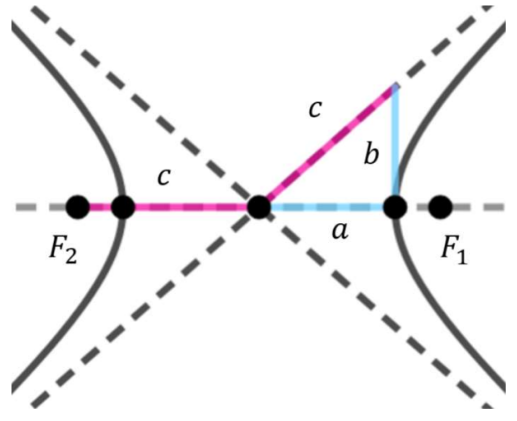
\includegraphics[width=5cm]{complexhyperbola.png}
				\end{minipage}
			\subsubsection{Intersections of Subsets}
				\begin{examquestion}{2006 NEAP Spesh E2 A8}
					\begin{leftbar}
						The values of $\Re(z),z\in\mathbb{C}$ such that $z$ belongs to $S\cap T$ where $S=\{z: |z-1|\leq 1\}$ and $T=\{z:\Re(z)+\Im(z)=1\}$ are
					\end{leftbar}
					Subset $T$ represents a line with the equation $x+y=1$ or $y=1-x$. Subset $S$ represents a circle with equation $(x-1)^2+y^2\leq1$. Substituting $1-x$ into the equation for $S$ and solving in CAS gives $\displaystyle 1-\frac{\sqrt{2}}{2}\leq x\leq\frac{\sqrt{2}}{2}+1$
				\end{examquestion}	
	\section{Logic and Proof}
		\subsection{Converses, Negations, Contrapositives}
			For a conditional statement $P\implies Q$:
			\paragraph{Negation} $P$ and $\neg Q$
				\subparagraph{de Morgan's Law} $\neg(P\land Q)\equiv\neg P\lor\neg Q$\\
				$\neg(P\lor Q)\equiv\neg P\land\neg Q$\\
				$\neg(P\implies Q)\equiv P\land \neg Q$
			\paragraph{Converse} $Q\implies P$
			\paragraph{Contrapositive} $\neg Q\implies\neg P$
			\begin{examquestion}{2023 Heffernan Spesh E2 A1}
				\begin{leftbar}
					Consider the following statement: 'If a number if a multiple of 6, then it is also a multiple of 3.' What is the \textbf{contrapositive} of this statement?
				\end{leftbar}
				P is 'multiple of 6' and Q is 'multiple of 3'. The contrapositive is $\neg Q\implies \neg P$, which is 'if a number is not a multiple of 3 then it is not a multiple of 6.'
			\end{examquestion}
		\subsection{Proof of Equivalent Statements}
			To prove $P\iff Q$ both $P\implies Q$ and $Q\implies P$ have to be shown to be true.
		\subsection{Proof by Contradiction}
			First, assume the statement is false, then show that this assumption leads to mathematical nonsense. Therefore we conclude that the assumption was wrong, and therefore the statement must be true.
		\subsection{Quantifiers and Counterexamples}
			\[
				\forall:\text{ 'For all'} \qquad \exists:\text{ 'There exists'}
			\]
			To prove universal statements ($\forall$) we need to provide a general argument that holds for every case in the set. To disprove universal statements, we need to provide a counterexample where it does not hold.\\
			To prove an existence statement ($\exists$) we need to show that it holds for at least one member in the set. To disprove these statements, we prove that its negation is true.
			\subsubsection{Negations with Quantifiers}
				Recall de Morgan's laws, apply these as normal and then flip the quantifier symbol ($\forall$ or $\exists$).
		\subsection{Product and Sum Notation}
			\[
				\sum_{i=1}^ni^2=1^2+2^2+...+n^2 \qquad \prod_{i=1}^n(2i-1)=1\times3\times5\times...\times(2n-1)
			\]
		\subsection{Direct Proof}
			\begin{examquestion}{1000 Spesh Questions Doc Proof 3}
				\begin{theorem*}
					There are no integers $a$ and $b$ such that $4a+8b=34$.
				\end{theorem*}
				\begin{proof}
					$4a+8b=34\implies 4(a+2b)=34$ and hence the statement is false as $\nexists k\in\mathbb{Z}\ni 34=4k$
				\end{proof}
			\end{examquestion}
		\subsection{Proof by Contradiction}
			To prove $P\implies Q$ by contradiction, we suppose the negation of the statement $\neg(P\implies Q)$ is true and show this results in nonsense.\\
			\begin{examquestion}{1000 Spesh Questions Doc Proof 2}
				\begin{theorem*}
					$\sqrt{3}+\sqrt{7}<2\sqrt{5}$
				\end{theorem*}
				\begin{proof}
					Suppose that $\sqrt{3}+\sqrt{7}\geq2\sqrt{5}$. By squaring both sides we get $3+2\sqrt{21}+7\geq20$.
					\begin{align*}
						10+2\sqrt{21}&\geq20\\
						\sqrt{21}&\geq{5}\\
						21&\geq25
					\end{align*}
					$21\geq25$ is a contradiction, and thus $\sqrt{3}+\sqrt{7}<2\sqrt{5}$
				\end{proof}
			\end{examquestion}
			\begin{examquestion}{1000 Spesh Questions Doc Proof 43}
				\begin{theorem*}
					$\cos\theta+\sin\theta\leq\sqrt{2}$
				\end{theorem*}
				\begin{proof}
					Suppose that $\cos\theta+\sin\theta>\sqrt{2}$.\\
					\begin{align*}
						\left(\cos\theta+\sin\theta\right)^2&>2\\
						\cos^2\theta+2\cos\theta\sin\theta+\sin^2\theta&>2\\
						1+\sin2\theta&>2\\
						\sin2\theta&>1
					\end{align*}
					As $\sin2\theta\in[-1,1]$, a contradiction has been reached, thus $\cos\theta+\sin\theta\leq\sqrt{2}$.
				\end{proof}
			\end{examquestion}
			\begin{examquestion}{1000 Spesh Questions Doc Proof 51}
				\begin{theorem*}
					The square root of an irrational number $m$ is also irrational.
				\end{theorem*}
				\begin{proof}
					Suppose that $\sqrt{m}=\frac{a}{b}\qquad a,b\in\mathbb{Z}\qquad m\notin\mathbb{Q}$.
					\[
						b^2m=a^2
					\]
					The RHS is an integer, but LHS is not since $m$ is by definition irrational. Hence a contradiction has been reached.\\
					Hence the square root of the irrational number $m$ is also irrational.
				\end{proof}
			\end{examquestion}
		\subsection{Arithmetic Mean-Geometric Mean Inequality}
			For $x,y\geq0$, the arithmetic mean is greater than or equal to the geometric mean.
			\[
				\frac{x+y}{2}\geq\sqrt{xy}
			\]
			\begin{example}{AM-GM Inequality}
				\begin{theorem*}
					For $a,b>0$ and $ab=24$, prove that $2a+3b\geq24$.
				\end{theorem*}
				\begin{proof}
					Assume $ab=24$, using the AM-GM inequality we find:\\
					\begin{align*}
						2a+3b&=\frac{4a+6b}{2}\\
						&\geq\sqrt{(4a)(6b)}=\sqrt{24ab}\\
						&=\sqrt{24\times24}\\
						&=24\\
						\\
						&\therefore 2a+3b\geq24\text{ as required.}
					\end{align*}
				\end{proof}
			\end{example}
		\subsection{Proof by Induction}
			\begin{examquestion}{University of Waikato Induction Problems Set Proof 18}
				\begin{theorem*}
					$5^{2n+1}+2^{2n+1}=7k,k\in\mathbb{Z}$ for all integers $n\geq0$.
				\end{theorem*}
				\begin{proof}
					\begin{itemize}[label=$\lozenge$, itemsep=4ex]
						\item \emph{Hypothesis}:
						\[
						P(n): 5^{2n+1}+2^{2n+1}=7k,k\in\mathbb{Z}
						\]
						\item \emph{Base case}:
						\[
							P(0): 5+2=7=7(1)\therefore\text{ holds}
						\]
						\item \emph{Inductive hypothesis}:
						\[
							\text{Assume }P(k)\text{ holds for all }k\in\mathbb{Z}^+\cup\{0\}: 5^{2k+1}+2^{2k+1}=7m,m\in\mathbb{Z}
						\]
						\item \emph{Inductive step}:
						\[
							P(k+1): 5^{2k+3}+2^{2k+3}=7x,x\in\mathbb{Z}
						\]
						\begin{align*}
							LHS=5^2\cdot5^{2k+1}+2^2\cdot2^{2k+1}&=25\cdot5^{2k+1}+4\cdot2^{2k+1}=4\left(5^{2k+1}+2^{2k+1}\right)+21\cdot5^{2k+1}\\
							&=4(7m)+7(3\cdot5^{2k+1})\\
							&=7(4m+3\cdot5^{2k+1})=7x
						\end{align*}
					\end{itemize}
					Therefore $(\forall k\in\mathbb{Z}^+\cup\{0\})P(k)\implies P(k+1)$\\
					By principle of mathematical induction, $P(n)$ holds for $n\geq0$.
				\end{proof}
			\end{examquestion}
			\begin{examquestion}{1000 Spesh Questions Doc Induction Proof 11}
				\begin{theorem*}
					$\displaystyle\sum_{r=1}^{n}\frac{1}{(r+1)(r+2)}=\frac{n}{2(n+2)}$ for $n\geq1$
				\end{theorem*}
				\begin{proof}
					\begin{itemize}[label=$\lozenge$, itemsep=4ex]
						\item \emph{Hypothesis}:
						\[
						P(n): \sum_{r=1}^{n}\frac{1}{(r+1)(r+2)}=\frac{n}{2(n+2)}
						\]
						\item \emph{Base case}:
						\begin{align*}
							P(1):\mathrm{LHS}=\qquad\sum_{r=1}^{1}\frac{1}{(r+1)(r+2)}&=\frac{1}{6}\\
							\mathrm{RHS}=\frac{1}{2(1+2)}&=\frac{1}{6}
						\end{align*}
						LHS=RHS $\therefore P(1)$ holds
						\item \emph{Inductive hypothesis}:
						\[
							\text{Assume }P(k)\text{ holds for all }k\in\mathbb{Z}\cap[1,\infty): \sum_{r=1}^{k}\frac{1}{(r+1)(r+2)}=\frac{k}{2(k+2)}
						\]
						\item \emph{Inductive step}:
						\[
							P(k+1): \sum_{r=1}^{k+1}\frac{1}{(r+1)(r+2)}=\frac{k+1}{2(k+3)}
						\]
						\begin{align*}
							\text{LHS}=\sum_{r=1}^{k+1}\frac{1}{(r+1)(r+2)}&=\sum_{r=1}^{k}\frac{1}{(r+1)(r+2)}+\frac{1}{(k+2)(k+3)}=\frac{k+1}{2(k+2)}+\frac{1}{(k+2)(k+3)}\\
							&=\frac{1}{k+2}\left(\frac{k}{2}+\frac{1}{k+3}\right)\\
							&=\frac{1}{2(k+2)}\left(\frac{k^2+3k+1}{2(k+3)}\right)=\frac{1}{2(k+2)}\left(\frac{(k+1)(k+2)}{k+3}\right)\\
							&=\frac{k+1}{2(k+3)}=\text{RHS}
						\end{align*}
						Therefore $(\forall k\in\mathbb{Z}\cap[1,\infty))P(k)\implies P(k+1)$ and therefore by the principle of mathematical induction, $P(n)$ holds for all integers $n\geq1$.
					\end{itemize}
				\end{proof}
			\end{examquestion}
			
	\section{Circular Functions}
		\subsection{Tech}
		
		\subsection{Inverse Circular Functions}
			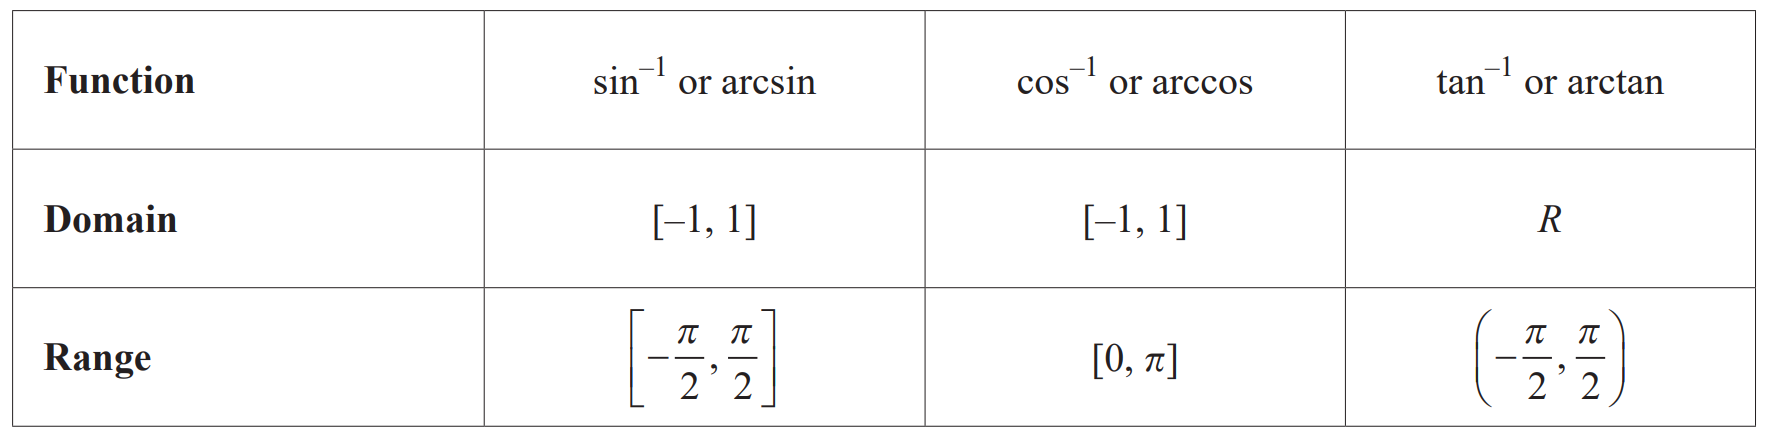
\includegraphics[width=\linewidth]{oldformulasheetinvtrig.png}
			\paragraph{arcsin function} when $y=\sin(x)$ is restricted to $x\in\left[-\frac{\pi}{2},\frac{\pi}{2}\right]$ the resulting function is one-to-one and therefore its inverse exists:
			\[
				\arcsin: [-1,1]\to\R,\arcsin(x)=y\qquad\text{where}\quad\sin(y)=x,y\in\left[-\frac{\pi}{2},\frac{\pi}{2}\right]
			\]
			\begin{minipage}{0.5\textwidth}
				\begin{itemize}
					\item domain of $\arcsin(x)$: $x\in[-1,1]$
					\item range of $\arcsin(x)$: $y\in\left[-\frac{\pi}{2},\frac{\pi}{2}\right]$
					\item $\arcsin(\sin(x))=x\forall x\in\left[-\frac{\pi}{2},\frac{\pi}{2}\right]$
					\item $\sin(\arcsin(x))=x\forall x\in[-1,1]$
				\end{itemize}
			\end{minipage}
			\hfill
			\begin{minipage}{0.4\textwidth}
				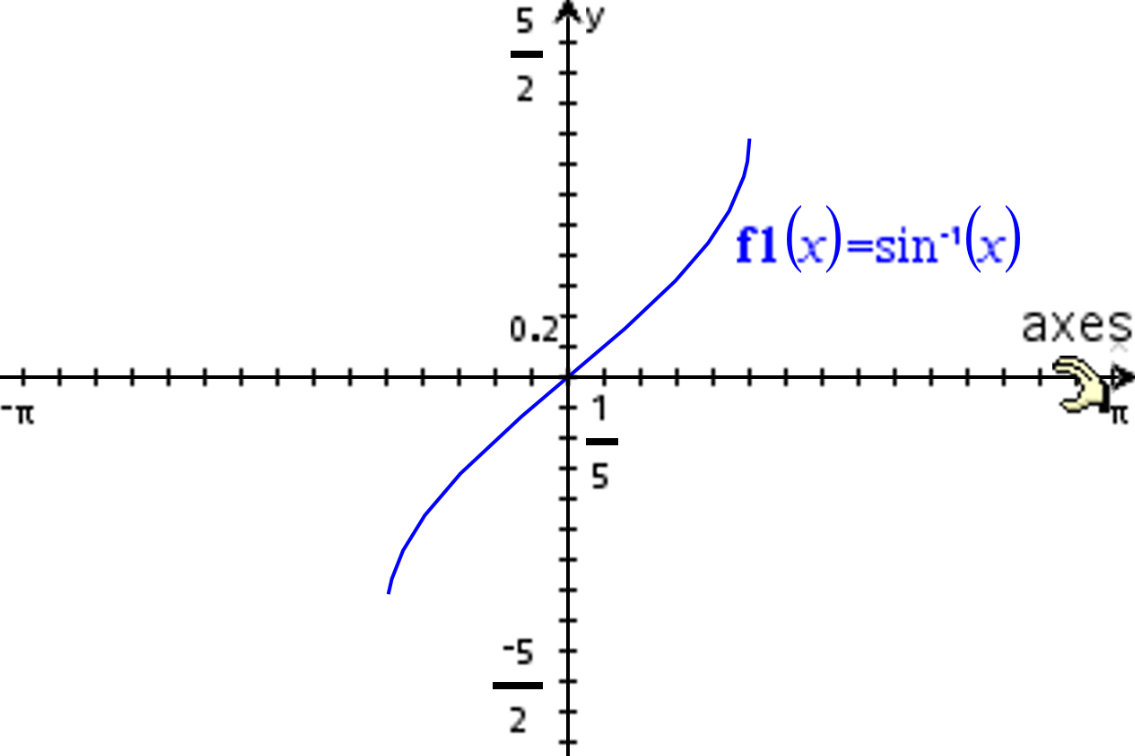
\includegraphics[width=\linewidth]{arcsin.png}
			\end{minipage}
		
			\paragraph{arccos function} when $y=\cos(x)$ is restricted to $x\in[0,\pi]$ the resulting function is one-to-one and therefore the inverse function exists.
			\[
				\arccos: [-1,1]\to\R,\arccos(x)=y\qquad\text{where}\quad\cos(y)=x,y\in[0,\pi]
			\]
			\begin{minipage}{0.5\textwidth}
				\begin{itemize}
					\item domain of $\arccos(x)$: $x\in[-1,1]$
					\item range of $\arccos(x)$: $y\in[0,\pi]$
					\item $\arccos(\cos(x))=x\forall x\in[-1,1]$
					\item $\cos(\arccos(x))=x\forall x\in[0,\pi]$
				\end{itemize}
			\end{minipage}
			\hfill
			\begin{minipage}{0.4\textwidth}
				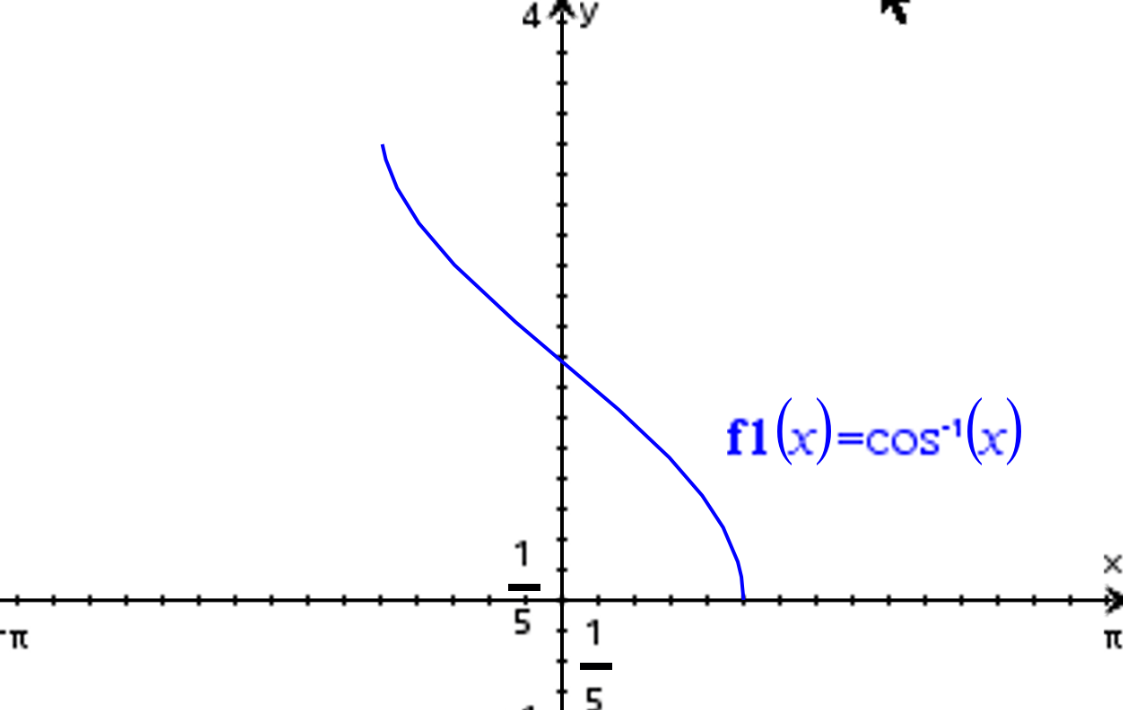
\includegraphics[width=\linewidth]{arccos.png}
			\end{minipage}
		
			\paragraph{arctan function} when $y=\tan(x)$ is restricted to $x\in\left(-\frac{\pi}{2},\frac{\pi}{2}\right)$ the resulting function is one-to-one and therefore the inverse function exists.
			\[
				\arctan: \R\to\R,\arctan(x)=y\qquad\text{where}\quad\tan(y)=x,y\in\left(-\frac{\pi}{2},\frac{\pi}{2}\right)
			\]
			\begin{minipage}{0.5\textwidth}
				\begin{itemize}
					\item domain of $\arctan(x)$: $x\in\R$
					\item range of $\arctan(x)$: $y\in\left(-\frac{\pi}{2},\frac{\pi}{2}\right)$
					\item $\arctan(\tan(x))=x\forall x\in\left(-\frac{\pi}{2},\frac{\pi}{2}\right)$
					\item $\tan(\arctan(x))=x\forall x\in\R$
				\end{itemize}
			\end{minipage}
			\hfill
			\begin{minipage}{0.4\textwidth}
				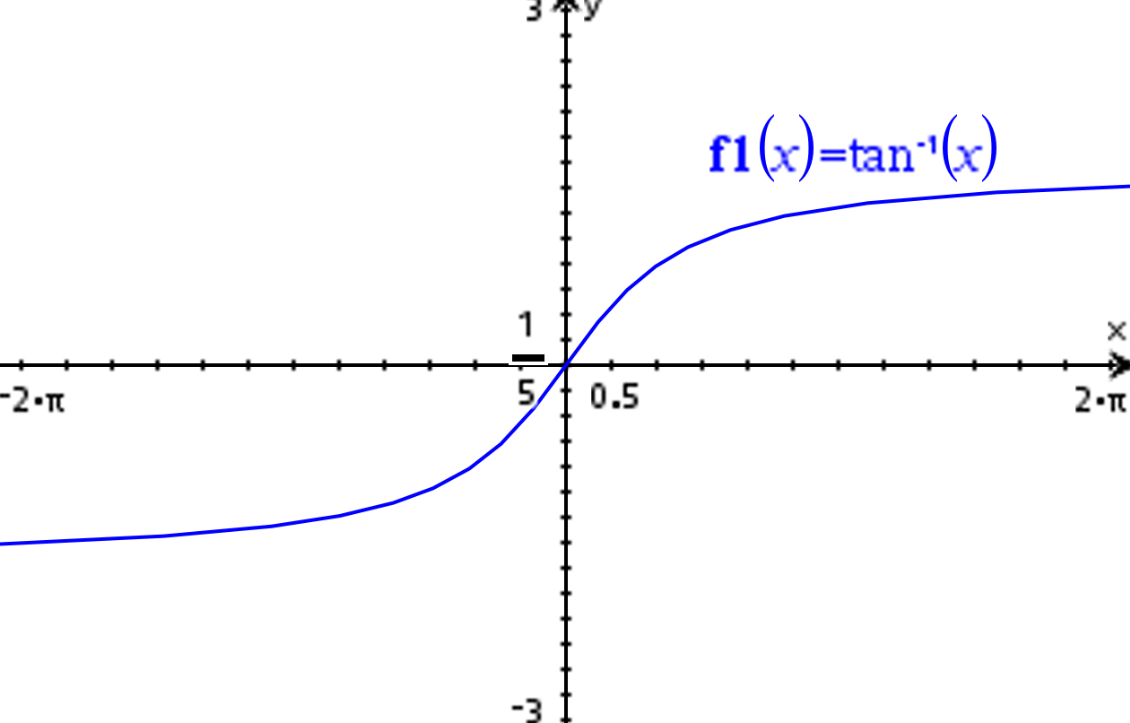
\includegraphics[width=\linewidth]{arctan.png}
			\end{minipage}
			\begin{examquestion}{2007 NEAP Spesh E2 A7}
				\begin{leftbar}
					The domain of $f(x)=\sin(2x)$ is restricted so that it is one-to-one. The domain and range of the resulting inverse $f^{-1}(x)$, could be respectively:
				\end{leftbar}
				The usual domain of $\sin(x)$ for one-to-one is $\left[-\frac{\pi}{2},\frac{\pi}{2}\right]$. The range of $\sin(x)$ is $[-1,1]$. The range is unchanged by the horizontal dilation, so the domain of $f^{-1}(x)$ will be $[-1,1]$. The domain of $\sin(2x)$ to be one-to-one will halve, so it could be $\left[-\frac{\pi}{4},\frac{\pi}{4}\right]$. Of the options, $\left[\frac{3\pi}{4},\frac{5\pi}{4}\right]$ is the only suitable option as it maintains the same period as $\left[-\frac{\pi}{4},\frac{\pi}{4}\right]$. Therefore the range of the inverse will be $\left[\frac{3\pi}{4},\frac{5\pi}{4}\right]$. Therefore \textbf{C}.
			\end{examquestion}
		\subsection{Symmetry Properties}
			\paragraph{Sine}
			\[
				-\sin(\alpha)=\sin(2\pi-\alpha)\qquad\sin(\pi-\alpha)=\sin(\alpha)\qquad\sin\left(\alpha+\frac{\pi}{2}\right)=\cos(\alpha)\qquad\sin\left(\alpha-\frac{\pi}{2}\right)=-\cos(\alpha)
			\]
			\paragraph{Cosine}
			\[
				-\cos(\alpha)=\cos(\pi-\alpha) \qquad \cos(2\pi-\alpha)=\cos(\alpha)\qquad\cos\left(\alpha-\frac{\pi}{2}\right)=\sin(\alpha)\qquad\cos\left(\alpha+\frac{\pi}{2}\right)=-\sin(\alpha)
			\]
			\paragraph{Tangent}
			\[
				\tan\left(\alpha+\frac{\pi}{2}\right)=\tan\left(\alpha-\frac{\pi}{2}\right)-\cot(\alpha)
			\]
			
		\subsection{Solutions of Equations with Circular Functions}
			\paragraph{Sine general solutions} For $a\in[-1,1]$ the general solution of $\sin(x)=a$ is:
			\[
				x=2n\pi+\arcsin(a)\qquad\text{or}\qquad x=(2n+1)\pi-\arcsin(a),n\in\mathbb{Z}
			\]
			\paragraph{Cosine general solutions} For $a\in[-1,1]$ the general solution of $\cos(x)=a$ is:
			\[
				x=2n\pi\pm\arccos(a),n\in\mathbb{Z}
			\]
			\paragraph{Tangent general solutions} For $a\in\R$ the general solution of $\tan(x)=a$ is:
			\[
				x=n\pi+\arctan(a),n\in\mathbb{Z}
			\]
		\subsection{Product-to-sum identities}
			\[
				2\cos(x)\cos(y)=\cos(x-y)+\cos(x+y) \qquad 2\sin(x)\sin(y)=\cos(x-y)-\cos(x+y) \qquad 2\sin(x)\cos(y)=\sin(x+y)+\sin(x-y)
			\]
		\subsection{Sum-to-product identities}
			\[
				\cos(x)+\cos(y)=2\cos\left(\frac{x+y}{2}\right)\cos\left(\frac{x-y}{2}\right) \qquad \cos(x)-\cos(y)=-2\sin\left(\frac{x+y}{2}\right)\sin\left(\frac{x-y}{2}\right)
			\]
			\[
				\sin(x)+\sin(y)=2\sin\left(\frac{x+y}{2}\right)\cos\left(\frac{x-y}{2}\right) \qquad \sin(x)-\sin(y)=2\sin\left(\frac{x-y}{2}\right)\cos\left(\frac{x+y}{2}\right)
			\]
	\section{Stats and Probability :skull:}
		\subsection{Tech}
			\subsubsection{sam\textunderscore prob\textbackslash bpd(n,p,lower,upper)} Outputs the probability distribution of a random binomial variable with $n$ trials and probability of success $p$ for a range of successes from lower to upper inclusive. It will also output the total probability of that range of successes.
			\subsubsection{sam\textunderscore prob\textbackslash pdanal({x},{px})}
			Fill in the values from the \textbf{discrete} probability distribution where the set {x} is the row of $x$ values and {px} is the row of $\Pr(X=x)$ values. It will tell you the mean and variance of that distribution.
			\subsubsection{scriptedmath\textbackslash expec(f(x),x)} Find the expected value of a continuous distribution with a density function f(x).
			\subsubsection{scriptedmath\textbackslash var(f(x),x)} Find the variance of a continuous distribution with a density function f(x).
			\subsubsection{scriptedmath\textbackslash sd(f(x),x)} Find the standard deviation of a continuous distribution with a density function f(x).
			\subsubsection{scriptedmath\textbackslash mode(list,freqlist)} Find the mode of list.
			\subsubsection{scriptedmath\textbackslash ns(eq,var)} Finds a relation to describe the non-negative integer solutions for the variable var to the equation.
			
			\subsubsection{normcdf(lower, upper, $\mu$, $\sigma$)} Finds the area under a normal density curve over an interval. For $\mathrm{Pr}(X\geq x)$ set the lower bound to be $x$ and the upper bound to be $\infty$. For $\mathrm{Pr}(X\leq x)$ set the upper bound to be $x$ and the lower bound to be $-\infty$. Input $\sigma$ and $\mu$ as given in the question.
			
			\subsubsection{invnorm(left tail prob, $\mu$, $\sigma$)} Used for solving $Pr(X>x_c)=C$. Input invnorm(1-$C$, $\mu$, $\sigma$) to get the value for $x_c$.
			
			\subsubsection{binomcdf(n, p, lower, upper)} Gives the $\Pr(lower<X<upper)$ for $X\sim\mathrm{Bi}(n,p)$.
			
			\subsubsection{binompdf(n, p, x)} Gives the $\Pr(X=x)$ for $X\sim\mathrm{Bi}(n,p)$.
			
			\subsubsection{invbinomn(cumulative prob, prob, numsuccess)} Menu+5+5+D. Inverse binomial with respect to $N$ (number of trials). Given the probability of success on each trial (prob), and the number of successes (numsuccesses), this function returns the minimum number of trials, $N$, such that for $X\sim\mathrm{Bi}(N,prob)$, that $\Pr(X<N)$ is less than cumulative probability.
			
			\subsubsection{sam\textunderscore prob\textbackslash normsum(x1,ltp1,x2,ltp2)}
			Find the mean and standard deviation of a normal distribution given the left-tail probability of two values. Put in one of the values for x1 and its left-tail probability for ltp1, and do the same for the second value.
			
			\subsubsection{Determine the Mean and Standard Deviation of a Normal Distribution}
				Suppose we have a normal distribution with mean 2 and unknown standard deviation, and we know that $\Pr(X>3)=0.3$. We first standardise to the standard normal random variable $Z\sim N(0,1^2)$. Using the left tail area (in this case 1-0.3=0.7) to find the percentile on the standard normal distribution, then solve this for $\displaystyle \frac{3-\mu}{\sigma}$ substituting appropriately to obtain the unknown standard deviation. The same process can be used for an unknown mean.
				\paragraph{Unknown Mean and Unknown Standard Deviation}
				Suppose $X\sim N(\mu,\sigma^2)$, but we know $\Pr(X>5)=0.65$ and $\Pr(X<1)=0.05$. Observe the following:
				\[
				\Pr(X>5)=\Pr\left(Z>\frac{5-\mu}{\sigma}\right)=0.65 \qquad \text{and} \qquad \Pr(X<1)=\Pr\left(Z<\frac{1-\mu}{\sigma}\right)=0.05
				\]
				We can then use \textbf{invnorm()} to find the z-scores of each equation above, and set up an appropriate system of equations to solve.
				\[
				\mathrm{invnorm}(1-0.65,0,1)=\frac{5-\mu}{\sigma} \qquad \text{and} \qquad \mathrm{invnorm}(0.05,0,1)=\frac{1-\mu}{\sigma}
				\]
			
			\subsubsection{Simulating Sample Means}
				randNorm($\mu$, $\sigma$, $n$) will give a list of $n$ values randomly selected in a normal distribution of mean $\mu$ and standard deviation $\sigma$. To find the sample mean apply mean() to this function.\\\\
				To do this for $m$ samples, add a \textbf{Lists and Spreadsheets} page in the CAS. In column A in the formula box input seq(mean(randNorm($\mu$,$\sigma$,$n$)),i,1,$m$). Remember $n$ is the sample size and $m$ is the number of samples. Name the column smeans. Now add a \textbf{Data and Statistics} page and add smeans to the $x$-axis.
			
			\subsubsection{Confidence Interval (Spesh)}
				To quickly find a confidence interval, in a calculator window go to menu+6+6+1. Set input method to stats, then input the necessary values.
			
			\subsubsection{Determine a Confidence Interval (Methods)}
				Menu+6+6+5 inserts the 1-Prop z interval function. Input the number of successes $x$, the sample size $n$, and the confidence level $C$.
				
				\begin{examquestion}{2016 VCAA Methods B3g}
					\begin{leftbar}
						A school has a class set of 22 new laptops kept in a recharging trolley. Provided each laptop is correctly plugged into the trolley after use, its battery recharges.\\\\
						On a particular day, a class of 22 students uses the laptops. All laptop batteries are fully charged at the start of the lesson. Each student uses and returns exactly one laptop. The probability that a student does not correctly plug their laptop into the trolley at the end of the lesson is 10\%. The correctness of any student’s plugging-in is independent of any other student’s correctness.\\\\
						The laptop supplier finds that, in a particular sample of 100 laptops, six of them have a battery life of less than three hours.\\\\
						Determine the 95\% confidence interval for the supplier's estimate of the proportion of interest. Give the values correct to two decimal places.
					\end{leftbar}
					\textbf{menu+6+6+5} then input successes=6, n=100, C=0.95
				\end{examquestion}
			
			\subsubsection{Hypothesis Testing - One Tail}
				Menu+6+7+1 $\to$ zTest. $\mu_0$ is the original population mean. $\sigma$ is the general standard deviation (do not divide by $\sqrt{n}$). $\bar{x}$ is the sample mean. $n$ is the sample size. Choose the type of alternative hypothesis and it will give you the necessary values.\\
				\textbf{For two tail-tests:} Do the same as for a one tail test, but choose the $\mu\neq\mu_0$ test type.
			\subsubsection{nSolve for brute force solving}
				In situations where solve() doesn't give a solution, even in approximate form, you can use nsolve() to brute force solve an equation.
				
			\subsubsection{Type II Error Probability}
				\paragraph{Instances of one-tail tests} For a 5\% significance one-tail hypothesis test, in order to calculate the probability of type II error use \textbf{invnorm(0.05,$\mu$,$\frac{\sigma}{\sqrt{n}}$)} to get the value for the sample mean which determines the boundary between rejection and acceptance of $H_0$. From this, execute a \textbf{normcdf(ans,$\infty$,true mean,$\frac{\sigma}{\sqrt{n}}$)} to find the probability of a Type II error.
				
				\paragraph{Instances of two-tail tests} For a 5\% significance two-tail hypothesis test, in order to calculate the probability of type II error use \textbf{invnorm(0.025,$\mu$,$\frac{\sigma}{\sqrt{n}}$)} to get the lower bound value for the 'acceptance region' and save this in a variable name like $l$. From this, do $\mu-l$ and save this as $d$ then $\mu+d$ (save this as $u$). Then execute \textbf{normcdf(l,u,true mean,$\frac{\sigma}{\sqrt{n}}$)} to find the probability of a Type II error.
			
		\subsection{Linear Functions of Random Variables}
			Consider a random variable $Y$ which is a linear function of random variable $X$
			\[
				Y=aX+b\qquad a,b\in\R
			\]
			
			\paragraph{Linear Functions of Discrete Random Variables} If $X$ is a discrete random variable $Y=aX+b$ is also a discrete random variable.
			
			\paragraph{Linear Functions of Continuous Random Variables} If $X$ is a continuous random variable, $Y=aX+b,a\neq0$ is also a continuous random variable. For $a>0$:
			\[
				\mathrm{Pr}(Y\leq y)=\mathrm{Pr}(aX+b\leq y)=\mathrm{Pr}\left(X\leq\frac{y-b}{a}\right)
			\]
			\[
				\therefore \mathrm{Pr}(Y\leq y)=\int\limits_{-\infty}^{\frac{y-b}{a}}f(x)dx
			\]
			
			\paragraph{Mean of Linear Functions of Random Variables}
				\subparagraph{Mean of Discrete Random Variables} For D.R.V's, the expected value $\mathrm{E}(X)$ of $X$ gives:
					\[
					\mathrm{E}(X)=\sum\limits_xx\cdot\mathrm{Pr}(X=x)
					\]
				\subparagraph{Mean of Continuous Random Variables} For C.R.V's, the expected value $\mathrm{E}(X)$ of $X$ gives:
					\[
					\mathrm{E}(X)=\int\limits_{-\infty}^{\infty}x\cdot f(x)dx
					\]
				For $Y=aX+b$:
				\[
					\mathrm{E}(Y)=\mathrm{E}(aX+b)=a\mathrm{E}(X)+b
				\]
			
			\paragraph{Variance of Linear Functions of Random Variables} Generally, for $X$ is a random variable with variance $\sigma^2$, and $Y=aX+b$ for $a,b\in\R$:
			\[
				\mathrm{Var}(Y)=a^2\mathrm{Var}(X)=a^2\sigma^2
			\]
			\[
				\mathrm{s.d}(Y)=\sqrt{a^2\sigma^2}=|a|\sigma
			\]
		\subsection{Independent Events}
			\[
				\text{Events }A,B\text{ are independent}\iff\Pr(A\cap B)=\Pr(A)\times\Pr(B)\qquad \Pr(A|B)=\Pr(A)
			\]
		\subsection{Mutually Exclusive Events}
			Two events A and B are mutually exclusive:
			\[
				\Pr(A\cap B)=0\qquad \Pr(A\cup B)=\Pr(A)+\Pr(B)
			\]
		\subsection{Linear Combination of Random Variables}
			The idea of independent events also applies to random variables. If two random variables' joint probability function is the product of their individual probability functions, the random variables are said to be independent.
			
			\paragraph{aX vs X+X+X+...+X} Consider $X$ representing the number that turns up on a dice roll. Then $2X$ is the result of one dice roll, doubled. $X+X$ is the the equivalent of rolling the dice twice and adding the results.
			\[
				\E(2X)=\E(X+X)=2\E(X)
			\]
			\[
				\mathrm{Var}(2X)=2^2\mathrm{Var}(X)=4\mathrm{Var}(X) \qquad \text{vs} \qquad \mathrm{Var}(X+X)=1^2\mathrm{Var}(X)+1^2\mathrm{Var}(X)=2\mathrm{Var}(X)
			\]
			
			\paragraph{Sum of Identically Distributed Independent Random Variables} Variables with the same mean and standard deviation and are independent. The events predicted by the random variables are also independent, so therefore we can find the sum of probabilities by multiplying the individual probabilities. Consider $X_1$ and $X_2$ being discrete random variables for two dice rolling.
			\[
				\mathrm{Pr}(X_1+X_2=2)=\mathrm{Pr}(X_1=1,X_2=2)=\mathrm{Pr}(X_1=1)\times\mathrm{Pr}(X_2=1)=\frac{1}{6}\times\frac{1}{6}=\frac{1}{36}
			\]
			\begin{examquestion}{2023 MAV Spec E2 QA20}
				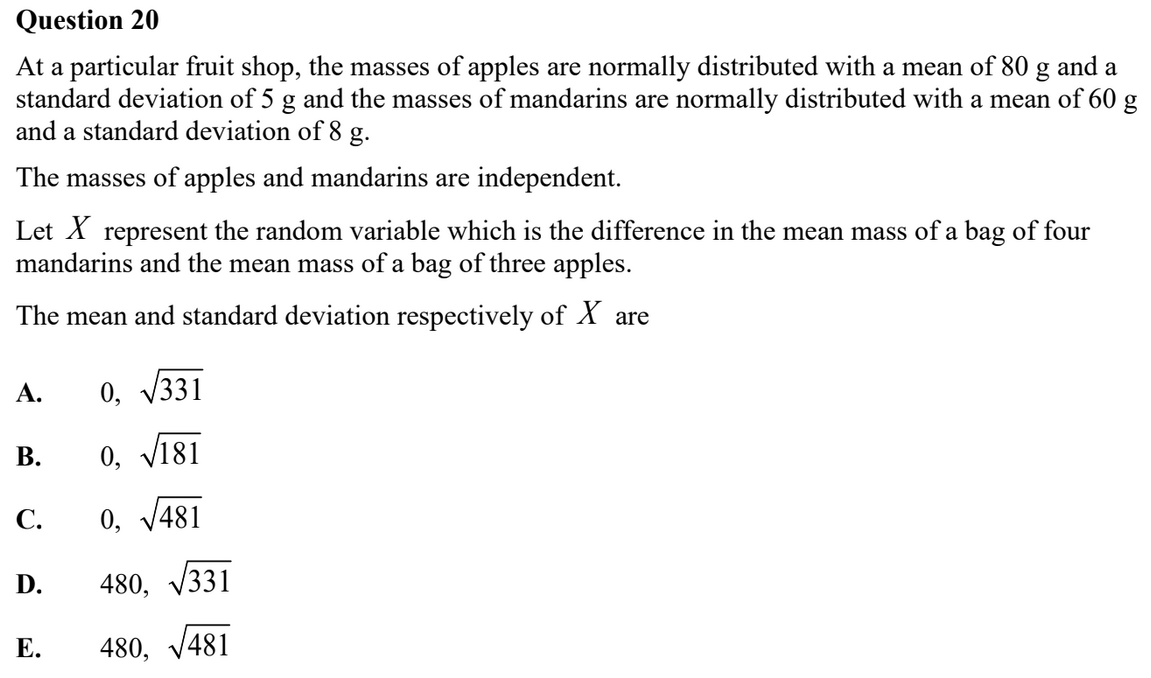
\includegraphics[width=\linewidth]{./img/2023mavspece2a20.png}
				\[
					\text{Let }X=M_1+M_2+M_3+M_4-(A_1+A_2+A_3)
				\]
				$\E(X)=4\times60-3\times80=0$ and $\mathrm{Var}(X)=4\times64+3\times25=331$. Therefore the answer is A.
			\end{examquestion}
			
			\paragraph{Mean of Sum of n Identically Distributed Independent Random Variables} $\displaystyle\mathrm{E}(X_1+X_2+...+X_n)=\mathrm{E}(X_1)+\mathrm{E}(X_2)+...+\mathrm{E}(X_n)=n\mu$
			
			\paragraph{Variance of Sum of n Identically Distributed Independent Random Variables} $\displaystyle\mathrm{Var}(X_1+X_2+...+X_n)=\mathrm{Var}(X_1)+\mathrm{Var}(X_2)+...+\mathrm{Var}(X_n)=n\sigma^2$\\
			$\displaystyle\mathrm{sd}(X_1+X_2+...+X_n)=\sqrt{\mathrm{Var}(X_1+X_2+...+X_n)}=\sqrt{n}\sigma$
			
			\paragraph{Linear Combinations of n Independent Random Variables} A random variable $Y$ which is a linear combination of random variables $X_1,X_2,...,X_n$ is given by $Y=a_1X_1+a_2X_2+...+a_nX_n$ for $a_1,a_2,...,a_n\in\R$.
			\[
				\mathrm{E}(a_1X_1+a_2X_2+...a_nX_n)=a_1\mathrm{E}(X_1)+a_2\mathrm{E}(X_2)+...+a_n\mathrm{E}(X_n)
			\]
			\[
				\mathrm{Var}(a_1X_1+a_2X_2+...+a_nX_n)=a_1^2\mathrm{Var}(X_1)+a_2^2\mathrm{Var}(X_2)+...+a_n^2\mathrm{Var}(X_n)
			\]
			\[
				\mathrm{sd}(a_1X_1+a_2X_2+...+a_nX_n)=\sqrt{a_1^2\mathrm{Var}(X_1)+a_2^2\mathrm{Var}(X_2)+...+a_n^2\mathrm{Var}(X_n)}
			\]
		
			\paragraph{Linear Combinations of Normal Random Variables} A linear combination of normally distributed random variables is also a normally distributed random variable.
		\subsection{Discrete Probability}
			\begin{examquestion}{2021 NEAP Methods MCQ 9}
				\begin{leftbar}
					A discrete random variable $X$ has the following probability distribution, where $k$ and $m$ are real constants.\\
					\resizebox{0.6\textwidth}{!}{
						\begin{tabular}{|c|c|c|c|c|c|}
							\hline
							$x$ & $0$ & $1$ & $2$ & $3$ \\
							\hline
							$\Pr(X=x)$ & $m$ & $k$ & $k-\frac{1}{4}$ & $k^2$ \\
							\hline
						\end{tabular}	
					}\mbox{}\\\\
					The maximum value of $m$ is:
				\end{leftbar}
				\begin{align*}
					&0\leq\Pr(X=2)\leq1\implies 0\leq k-\frac{1}{4}\leq1\\
					\therefore&k_{min}=\frac{1}{4}\\
					m&=1-\left(\frac{1}{4}+0+\frac{1}{4}^2\right)\\
					&=\frac{11}{16}
				\end{align*}
			\end{examquestion}
			\begin{examquestion}{2016 VCAA Methods MCQ 19}
				\begin{leftbar}
					Consider the discrete probability distribution with random variable $X$ below:\\
					\resizebox{0.6\textwidth}{!}{
						\begin{tabular}{|c|c|c|c|c|c|}
							\hline
							$x$ & $-1$ & $0$ & $b$ & $2b$ & $4$ \\
							\hline
							$\Pr(X=x)$ & $a$ & $b$ & $b$ & $2b$ & $0.2$ \\
							\hline
						\end{tabular}	
					}\mbox{}\\\\
					The smallest and largest possible values of $\E(X)$ are:
				\end{leftbar}
				\begin{align*}
					\E(X)&=-a+b^2+4b^2+0.8=0.8+5b^2-a \\
					&a+4b+0.2=1\to a+4b=0.8 \\
					\E(X)&=0.8+5b^2-(0.8-4b)=5b^2+4b=b(4+5b) \\
					&\text{Parabola with intercept } b=0,b>0\\
					\therefore\E_{min}(X)&=0\\
					&0\leq a\leq 0.8 \to 0\leq0.8-4b\leq0.8\\
					&\implies -0.8\leq-4b\leq0 \to 0.2\geq b\geq0\\
					&\text{Taking maximum value of b: }b=0.2\\
					\therefore\E_{max}(X)&=0.2\cdot(4+5\cdot0.2)=1
				\end{align*}
			\end{examquestion}
		\subsection{Normal Probability}
			\[
			X\sim N(\mu,\sigma^2)
			\]
			\paragraph{Symmetry Properties of Normally Distributed Probabilities} Consider $Z\sim\mathrm{N}(0,1)$.
			\begin{itemize}
				\item $\Pr(Z>a)=1-\Pr(Z\leq a)$
				\item $\Pr(Z<-a)=\Pr(Z>a)$
				\item $\Pr(-a<Z<a)=1-2\Pr(Z\geq a)=1-2\Pr(Z\leq -a)$
			\end{itemize}
			\begin{examquestion}{2010 NEAP Methods E2 B3}
				\begin{leftbar}
					A winery produces bottles of wine in two sizes: standard and large. For each size, the content of the bottles are normally distributed according to the following:\\
					\begin{tabular}{|c|c|c|}
						\hline
						\textbf{Bottle Size} & \textbf{Mean} & \textbf{Standard Deviation} \\
						\hline
						standard & 0.760 & 0.008 \\
						\hline
						large & $\mu$ & $\sigma$ \\
						\hline
					\end{tabular}\mbox{}\\
					The probability that a randomly selected standard bottle contains fewer than 0.750 litres of wine is known to be 0.1056. Of the large bottles, 8\% contain more than 1.023 litres and 4\% contain less that 0.994 litres. Show that the mean and standard deviation of the large bottles can be found by solving the system of equations: $\mu+1.4051\sigma=1.023$ and $\mu-1.7507\sigma=0.994$.
				\end{leftbar}
				\begin{align*}
					&X\sim N(\mu,\sigma^2) \qquad \Pr(X>1.023)=0.08 \qquad \Pr(X<0.994)=0.04 \\
					&Z\sim N(0,1)\\
					&\Pr(X>1.023)=\Pr\left(Z>\frac{1.023-\mu}{\sigma}\right)=0.08 \qquad \textbf{invnorm(0.92,0,1) gives } \frac{1.023-\mu}{\sigma}=1.4051 \text{ standard deviations}\\
					&\Pr(X<0.994)=\Pr\left(Z<\frac{0.994-\mu}{\sigma}\right)=0.04\qquad \textbf{invnorm(0.04,0,1) gives } \frac{0.994-\mu}{\sigma}=-1.7507 \text{ standard deviations}\\
					\therefore &\mu+1.4051\sigma=1.023\\
					&\mu-1.7507\sigma=0.994 \text{ as required}
				\end{align*}
			\end{examquestion}
			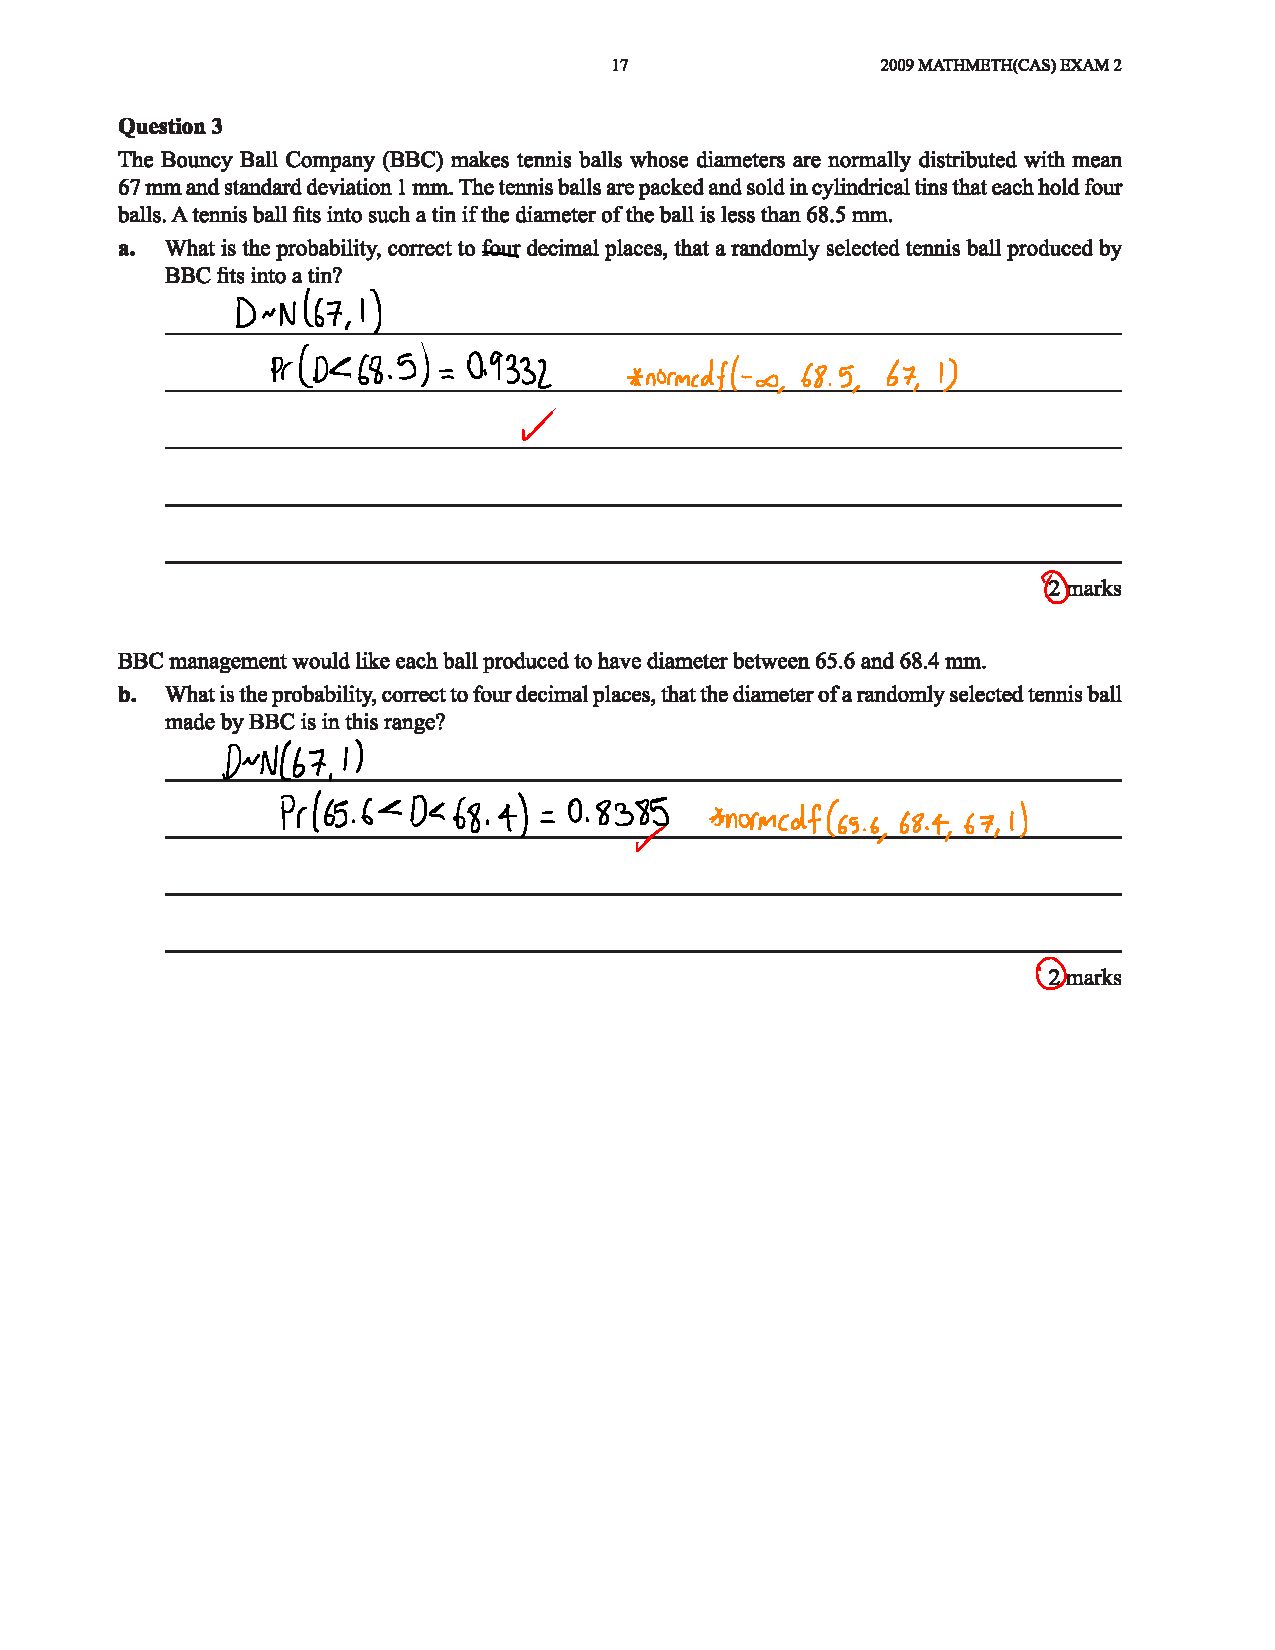
\includepdf[pages={1,2,3}]{./pdf/2009e2mmq3.pdf}
		\subsection{The Binomial Distribution}
			\paragraph{Bernoulli Sequence} describes a sequence of trials for which there are two possible outcomes (success, failure), the probability of success $p$ is constant for all trials, and the trials are independent. The number of successes in a Bernoulli sequence of $n$ trials is called a Binomial Random Variable denoted $X\sim \mathrm{Bi}(n,p)$
			\begin{examquestion}{Suzanne Cory 2018 SAC3 Part II Q2e/f}
				\begin{leftbar}
					In an isolated incident, Ricardo got his CAS stolen when he left it unattended in a breakout room in the G16-21 area after school one day. He found it later being sold on Gumtree.\\
					Chelsea, from his homegroup, thinks she saw who walked into the breakout room. However, she was sitting quite far away, and her accusations are flimsy at best. To verify her claim, Mr. Mott tested her eyesight, by assessing her ability to identify a student from the claimed distance away.\\
					The probability that she would correctly identify a student is 0.8. In the test to identify 8 students from distance, B is the random variable following a binomial distribution for the number of students she identifies correctly.\\\\
					e) What is the probability the she identified exactly 7 students correctly, given that she correctly identified the first two (give your answer to 4dp).
				\end{leftbar}
				We know $B\sim\mathrm{Bi}(8,0.8)$ We know the outcomes of two out of eight trials, both being successes. So we can treat this as a binomial variable $B_1\sim\mathrm{Bi}(2,0.8)$, we then treat the remaining 6 trials as a binomial variable $B_2\sim\mathrm{Bi}(6,0.8)$.
				\[
					\Pr(B=7|\text{first two are correct})=\Pr(B_2=5|B_1=2)=\frac{\Pr(B_2=5)\times\Pr(B_1=2)}{\Pr(B_1=2)}
				\]
				\[
					\frac{\Pr(B_2=5)\times\Pr(B_1=2)}{\Pr(B_1=2)}=\Pr(B_2=5)=0.3932\qquad\textbf{binompdf(6,0.8,5)}
				\]
				\begin{leftbar}
					f) What is the minimum number of students in the test to ensure that the probability of Chelsea identifying at least 7 of them is 0.46?
				\end{leftbar}
				\begin{align*}
					&X\sim\mathrm{Bi}(n,0.8)\\
					&\Pr(X\geq7)\geq0.46\\
					\implies&\Pr(X\leq6)\leq0.54\\
					\implies&n=8\qquad\textbf{invBinomN(0.54,0.8,6)}
				\end{align*}
			\end{examquestion}
			\subsubsection{Inverse Binomial}
			\begin{examquestion}{2008 VCAA Methods MCQ 5}
				\begin{minipage}{\linewidth}
					\begin{leftbar}
						Let $X$ be a discrete random variable with a binomial distribution. The mean of $X$ is 1.2 and the variance of $X$ is 0.72. The values of $n$ (the number of independent trials) and $p$ (the probability of success in one trial) are:
					\end{leftbar}
				\end{minipage}
				\begin{align*}
					\mu&=np=1.2 \\
					\sigma^2&=np(1-p) \\
					&\text{Solving the system gives }n=3,p=0.4
				\end{align*}
			\end{examquestion}
			\begin{examquestion}{2022 VCAA NHT Methods QB4f}
				\begin{leftbar}
					The proportion of custard doughnuts as a proportion of all doughnuts made in the bakery is 0.44. Find the minimum number of doughnuts required in a box to ensure that the probability of having at least 12 custard doughnuts in a box is greater than 90\%.
				\end{leftbar}
				\textbf{invBinomN(0.1,0.44,11)} gives 35, the minimum number of doughnuts. Cumulative probability is 1-0.9=0.1. Probability of success if the proportion, and the number of successes is one less than the threshold (12).
			\end{examquestion}
		\subsection{Sample Means}
			\paragraph{Populations and samples}
				\begin{itemize}
					\item \textbf{Population} is the set of all eligible members of the intended group of study.
					\item \textbf{Sample} is a subset of the population which is selected to make inferences about the population.
					\item The \textbf{population mean} $\mu$ is the mean of all values of a measure in the entire population.
					\item The \textbf{sample mean} $\bar{x}$ is the mean of the values of measure in a particular sample. Since this varies based on the contents of a random sample, we consider $\bar{x}$ as being values of a random variable $\bar{X}$
				\end{itemize}
			
			\paragraph{Sample Mean of a normal random variable} Let $X$ be a normally distributed random variable with mean $\mu$ and standard deviation $\sigma$. Let $X_1,X_2,...,X_n$ represent a sample size of $n$ selected from this population. The sample mean is defined as:
			\[
				\bar{X}=\frac{X_1+X_2+...+X_n}{n}
			\]
			The sample mean $\bar{X}$ is normally distributed with $\mathrm{E}(\bar{X})=\mu$ and $\mathrm{sd}(\bar{X})=\frac{\sigma}{\sqrt{n}}$.
			
			\begin{example}{Edrolo Sample Mean MCQ}
				\begin{leftbar}
					The diameter, in metres, of trees in a certain forest is distributed with the following density function:
					\[
						g(x)=\frac{12}{2401}(x-3)(x-10)^2,3\leq x\leq 10
					\]
					Find the probability that the mean diameter of a sample of 40 trees is less than 6m to 2 decimal places.
				\end{leftbar}
				Let $G$ be the random variable representing the diameter of a randomly selected tree. The sample size is large enough that the distribution of sample means will be approximately normal.\\
				\[
					\E(G)=\int\limits_3^{10}x\times\frac{12}{2401}(x-3)(x-10)^2dx=\frac{29}{5}
				\]
				\[
					\mathrm{Var}(G)=\E(G^2)-[\E(G)]^2=\int\limits_3^{10}x^2\times\frac{12}{2401}(x-3)(x-10)^2dx-(\frac{29}{5})^2=\frac{49}{25}
				\]
				We use these results to find the distribution of $\bar{G}$.\\
				\[
					\E(\bar{G})=\E(G)=\frac{29}{5}
				\]
				\[
					\mathrm{sd}(\bar{G})=\frac{\mathrm{sd}(G)}{\sqrt{40}}=\frac{7}{5\sqrt{40}}=\frac{7}{10\sqrt{10}}
				\]
				For $\Pr(\bar{G}<6)$, we can use \textbf{normcdf(-$\infty$,6,$\E(\bar{G})$,$\mathrm{sd}(\bar{G})$)}, which gives $\Pr(\bar{G}<6)=0.82$
			\end{example}
				
		\subsection{Normal Approximation of Sample Proportions}
			The distribution of the sample mean $\bar{X}$ is normal with mean $\bar{x}=\mu$ and the standard deviation $s=\frac{\sigma}{\sqrt{n}}$.
			\[
				\Pr\left(\bar{X}>a\right)=\Pr\left(Z>\frac{a-\bar{x}}{s}\right) \qquad Z\sim(0,1)
			\]
			\begin{example}{FreeVCENotes Normal Approximation}
				\begin{leftbar}
					Use the normal approximation to the binomial distribution to find the approximate probability, to 4 decimal places, that in the next 600 rolls of a fair die, the proportion of sixes rolled is less than 0.2.
				\end{leftbar}
				\begin{align*}
					&\text{Let }\hat{P}\text{ be the proportion of sixes rolled}\\
					\E(\hat{P})&=p=\frac{1}{6}\\
					\mathrm{sd}(\hat{P})&=\sqrt{\frac{p(1-p)}{n}}=\sqrt{\frac{\frac{1}{6}\left(\frac{5}{36}\right)}{600}}\\
					&=\sqrt{\frac{1}{4320}}\\\\
					\hat{P}\sim&N\left(\frac{1}{6},\sqrt{\frac{1}{4320}}\right)\\
					\Pr(\hat{P}<0.2)&=\textbf{normcdf}\left(0,0.2,\frac{1}{6},\sqrt{\frac{1}{4320}}\right)\\
					&=0.9858
				\end{align*}
			\end{example}
		\subsection{Sample Proportions $\hat{P}$ without Normal Approximation (Methods)}
			\paragraph{Mean, Variance, Standard Deviation} Using the mean and variance from the binomial, we can derive the following about the sample proportion $\hat{P}$:\\
			\[
				\hat{P}=\frac{X}{n},\quad X\sim\mathrm{Bi}(n,p)
			\]
			\[
				\E(\hat{P})=p\qquad \mathrm{Var}(\hat{P})=\frac{p(1-p)}{n}\qquad \mathrm{sd}(\hat{P})=\sqrt{\mathrm{Var}(\hat{P})}
			\]
			\begin{examquestion}{2016 VCAA Methods A17}
				\begin{minipage}{\linewidth}
					\begin{leftbar}
						Inside a container there are one million coloured building blocks. It is known that 20\% of the blocks are red. A sample of 16 blocks is taken from the container. For samples of 16 blocks, $\hat{P}$ is the random variable of the distribution of sample proportions of red blocks. \textbf{(Do not use a normal approximation.)}
					\end{leftbar}
				\end{minipage}\mbox{}\\\\
				Let $X\sim Bi(16,0.2)$ be a binomial variable representing the number of red blocks in the sample.
				\[
				\hat{P}=\frac{X}{16}\implies X=16\hat{P}
				\]
				\begin{align*}
					\Pr\left(\hat{P}\geq\frac{3}{16}\right)&=\Pr\left(X\geq\frac{3}{16}\times16\right)& \\
					&=0.6482&\textbf{binomcdf(16,0.2,3,16)}
				\end{align*}
			\end{examquestion}
			\begin{examquestion}{2016 VCAA Methods E2 B3d}
				\begin{leftbar}
					A supplier of laptops decides to take a sample of 100 new laptops from a number of different schools. For samples of size 100 from the population with a mean battery life of 3 hours 10 minutes and a standard deviation of 6 minutes, $\hat{P}$ is the random variable of the distribution of sample proportions of laptops with battery life less than three hours. It is known that the probability that the probability that a single laptop's battery life is less than 3 hours is 0.0478. Find $Pr(\hat{P}\geq0.06|\hat{P}\geq0.05)$ without a normal approximation.
				\end{leftbar}
				\begin{align*}
					&\text{Let } Y\text{ be the number of laptops with battery less than 3 hours} \\
					&Y\sim\mathrm{Bi}(100,0.0478)\\
					&\hat{P}=\frac{Y}{100}\implies\Pr\left(\hat{P}\geq0.06|\hat{P}\geq0.05\right)=\Pr\left(Y\geq0.06\times100|Y\geq0.05\times100\right)\\
					&=\Pr\left(Y\geq6|Y\geq5\right)\\
					&=\frac{\Pr(Y\geq6)}{\Pr(Y\geq5)}=0.658
				\end{align*}
			\end{examquestion}
			
		\subsection{Distribution of the sample mean}
			\subsubsection{Central Limit Theorem} Let $X$ be any random variable with mean $\mu$ and standard deviation $\sigma$. Then, provided that the sample size $n$ is large enough, the distribution of $\bar{X}$ is approximately normal with mean $\mathrm{E}(\bar{X})=\mu$ and $\mathrm{sd}(\bar{X})=\frac{\sigma}{\sqrt{n}}$.
			
			\subsubsection{Normal Approximation to the Binomial Distribution} If $X$ is a binomial random variable with parameters $n,p$, then the distribution of $X$ is approximately normal with mean $\mu=np$ and standard deviation $\sigma=\sqrt{np(1-p)}$ provided $np>5$ and $n(1-p)>5$.
			
		\subsection{Confidence Intervals for the Population Mean}
			\paragraph{Interpretation of a Confidence Interval} For a 95\% confidence interval, we expect 95\% of such intervals to contain the population mean $\mu$. Whether or not a particular confidence interval contains $\mu$ is generally unknown.
			
			\paragraph{Point Estimates} The value of the sample mean $\bar{x}$ can be used to estimate the population mean $\mu$, as this is a single-valued estimate, it is called a point estimate of $\mu$.
			
			\paragraph{Interval Estimates} An interval estimate for the population mean $\mu$ is called a confidence interval for $\mu$.
				\subparagraph{C\% Confidence Interval} An approximate $C\%$ confidence interval for $\mu$ is given by
				\[
					\left(\bar{x}-z\frac{\sigma}{\sqrt{n}},\bar{x}+z\frac{\sigma}{\sqrt{n}}\right)
				\]
				where $z\ni\mathrm{Pr}(-z<Z<z)=C\%$, $\bar{x}$ is the sample mean, $\sigma$ is the standard deviation of the population and $n$ is the size of the sample from which $\bar{x}$ was calculated.\\\\
				
				\begin{minipage}{0.5\textwidth}
					The values of $z$ for common confidence intervals:
					\begin{itemize}
						\item 90\% $\to z=1.6449$
						\item 95\% $\to z=1.9600$
						\item 99\% $\to z=2.5758$
					\end{itemize}
				\end{minipage}
				\hfill
				\begin{minipage}{0.5\textwidth}
					To find the $z$ score to use for any $C\%$ confidence interval in CAS: \textbf{invnorm($\frac{C}{2}$,0,1)} will give you the value for $z$.
				\end{minipage}
				
				
				
			\begin{examquestion}{VCAA Spesh 2017 Exam 2 A19}
				\begin{leftbar}
					A confidence interval is to be used to estimate the population mean $\mu$ based on a sample mean $\bar{x}$. To decrease the width of a confidence interval by $75\%$, the sample size must be multiplied by a factor of...
				\end{leftbar}
				To reduce by 75\% is the equivalent to making it a quarter the width, i.e. dividing by four:
				\begin{align*}
					\frac{\sigma}{4\sqrt{n}}=\frac{\sigma}{\sqrt{16n}}
				\end{align*}
				Therefore the sample size must be multiplied by a factor of 16.
			\end{examquestion}
			\begin{examquestion}{2023 MAV Methods E2 A16}
				\begin{leftbar}
					A survey found that 110 out of 400 Year 12 students study more than 2 hours per night. An approximate 95\% confidence interval for the proportion of Year 12 students who study more than 2 hours per night is $(0.2312,0.3188)$. If the width of this confidence interval was to be decreased by 70\%, the sample size must be:
				\end{leftbar}
				\begin{minipage}{0.5\textwidth}
					\begin{align*}
						W_1=2z\frac{\sigma}{\sqrt{n_1}},&W_2=2z\frac{\sigma}{\sqrt{n_2}}\\
						W_2=2z\frac{\sigma}{\sqrt{n_2}}&=0.3\times2z\frac{\sigma}{\sqrt{n_1}}\\
						\frac{1}{\sqrt{n_2}}&=0.3\frac{1}{\sqrt{n_1}}\\
						\implies n_2&=\frac{100}{9}n_1
					\end{align*}
				\end{minipage}
				\begin{minipage}{0.5\textwidth}
					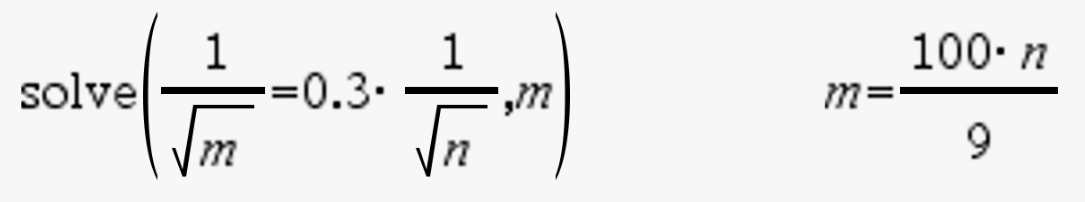
\includegraphics[width=\textwidth]{./img/mavmm2023a16.png}
					Where $m$ is the new sample size and $n$ is the original sample size.
				\end{minipage}
				The sample size must be increased by a factor of $\frac{100}{9}$
			\end{examquestion}
		\subsection{Hypothesis Testing for Mean}
			\paragraph{Null hypothesis} The null hypothesis is denoted by $H_0$ says that the sample is drawn from a population which has the same mean as before (the mean has not changed after taking the sample). Under this hypothesis, any difference between a sample statistic and a population parameter is explained by sample-sample variation.
			
			\paragraph{Alternative hypothesis} The alternative hypothesis $H_1$ says that the population mean has changed.
			
			\paragraph{p-Values} The $p$ value is the probability of observing a value of the sample statistic as extreme as or more extreme than the one observed, assuming that the null hypothesis is true.
			
			\paragraph{Statistical Significance} The significance level represents the threshold of unlikelihood that a result must have to cast sufficient doubt on the null hypothesis. This is denoted by $\alpha$.
			
			If the $p$-value is less than $\alpha$, we reject the null hypothesis in favour of the alternative hypothesis. If the $p$-value is greater than $\alpha$, we do not reject the null hypothesis.
			
			\paragraph{z-test} is the name for the hypothesis test for a mean of a sample drawn from a normally distributed population with known standard deviation.
			
			\subsubsection{One-tail tests}
				For directional alternative hypotheses, one-tail tests are used to calculate $p$-values.\\
				For $H_1:\mu>x$ the p-value is calculated considering only values in the upper tail of the normal curve.\\
				For $H_1:\mu<x$ the p-value is calculated considering only values in the lower tail of the normal curve.\\
			\subsubsection{Two-tail tests}
				Non-directional alternative hypothesis $p$-values are determined with two-tail tests. $H_1:\mu\neq x$.\\
				\[
					p=\Pr\left(\left|\bar{X}-\mu\right|\geq\left|\bar{x}-\mu\right|\right)
				\]
				$p$-value (two-tail)=2$\times p$-value (one-tail)
				\begin{example}{Cumbridge Modulus Bullshit}
					\begin{leftbar}
						Suppose that the weight $X$kg of sand in a bag is a normally distributed random variable with a mean of 50kg and a standard deviation of 1.5kg. A random sample of 10 bags is taken.\\
						a) Find the probability that the mean weight of the 10 bags in the sample differs by 1kg or more from the population mean.
					\end{leftbar}
					\begin{align*}
						\Pr\left(\left|\bar{X}-\mu\right|\geq1\right)&=\Pr\left(\left|\frac{\bar{X}-\mu}{\sigma/\sqrt{n}}\right|\geq\frac{1}{\frac{1.5}{\sqrt{10}}}\right)\\
						&=\Pr\left(\left|Z\right|\geq2.108 \right)\\
						&=2\times\Pr(Z\leq-2.108)\\
						&=0.035
					\end{align*}
					\begin{leftbar}
						b) Suppose that the mean weight of the 10 bags is 49.1kg\\
						i) Determine the $p$ value appropriate to the following hypotheses:\\
						\begin{equation*}
							H_0:\mu=50\qquad H_1:\mu\neq50
						\end{equation*}
					\end{leftbar}
					\begin{align*}
						p&=\Pr\left(\left|\bar{X}-\mu\right|\geq\left|\bar{x}-\mu\right|\right)\\
						&=\Pr\left(|Z|\geq\left|\frac{49.1-50}{1.5/\sqrt{10}}\right|\right)\\
						&=\Pr\left(|Z|\geq|-1.897|\right)\\
						&=2\Pr\left(Z\geq1.897\right)=0.0578
					\end{align*}
					\begin{leftbar}
						ii) What is your conclusion at $\alpha=0.05$?
					\end{leftbar}
					Since $p$ is greater than $\alpha$, there is insufficient evidence to conclude that the mean weight of the bags is not 50kg.
				\end{example}
			\subsubsection{Relation to Confidence Intervals}
				Consider the fact of the real number line:
				\[
					a\in\left(b-c,b+c\right)\iff|a-b|<c\iff b\in(a-c,a+c)
				\]
				Suppose we have:
				\[
					H_0:\mu=\mu_0 \qquad H_1:\mu\neq\mu_0
				\]
				Then:
				\[
					\mu_0\notin\left(\bar{x}-1.96\frac{\sigma}{\sqrt{n}},\bar{x}+1.96\frac{\sigma}{\sqrt{n}}\right)\iff\bar{x}\notin\left(\mu_0-1.96\frac{\sigma}{\sqrt{n}},\mu_0+1.96\frac{\sigma}{\sqrt{n}}\right)
				\]
				Hence the 95\% confidence interval does not contain $\mu_0$ if and only if we should reject $H_0$ at a $5\%$ significance.
			\subsubsection{Hypothesis Testing Errors}
				\paragraph{Type I} Rejecting the null hypothesis when it is true. $\Pr$(Type I)$=\Pr(H_0 \text{ rejected}|H_0 \text{ true})=\text{ level of significance of test}$
				\paragraph{Type II} Not rejecting the null hypothesis when it is false. $\Pr$(Type II)$=\Pr(H_0 \text{ not rejected}|H_0 \text{ false})$
				\begin{examquestion}{VCAA 2023 Specialist E2 Sample Q7}
					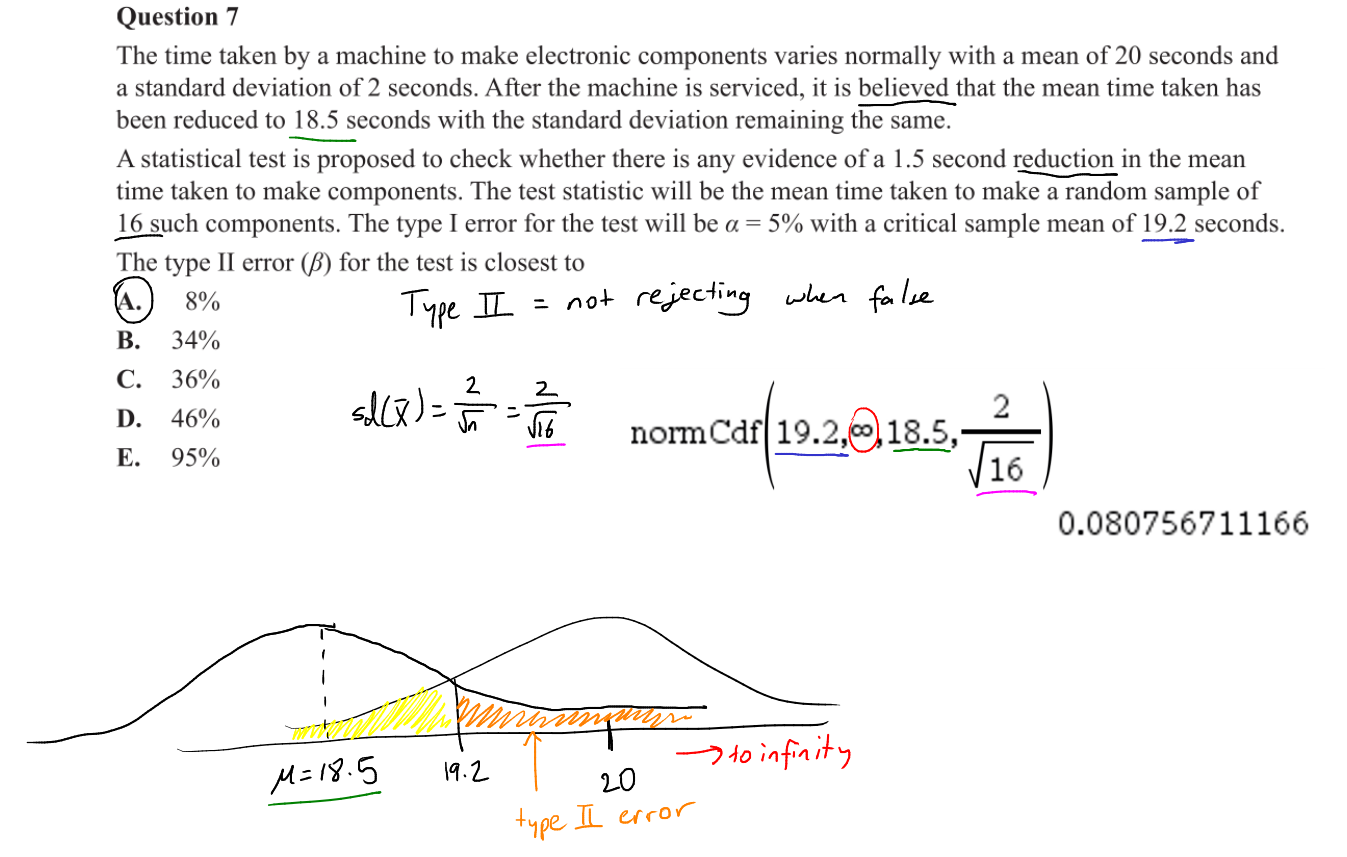
\includegraphics[width=\textwidth]{./img/spectypeii.png}
				\end{examquestion}
				\begin{examquestion}{Heffernan 2023 Spesh E2 A20}
					\begin{leftbar}
						A battery company claims that their Type A battery has an average lifetime of 1000 hours and a standard deviation of 100 hours. Unconvinced of the company’s claim, a consumer rights organisation conducts a one-tailed statistical test at the 1\% level of significance and obtains a random sample of 50 Type A batteries.\\
						If the actual average lifetime of a Type A battery is 950 hours, the probability of making a type II error is...
					\end{leftbar}
					Recall that $\Pr(type II)=\Pr(Accept H_0 | H_0 false)$.\\
					First, we need to find the critical sample mean, that is the value of $a$ such that $\Pr(\bar{X}<a|\mu=1000)=0.01$ (rejecting the null hypothesis). Using CAS we find $a=967.1005$, then we use this info to find the type II error.\\
					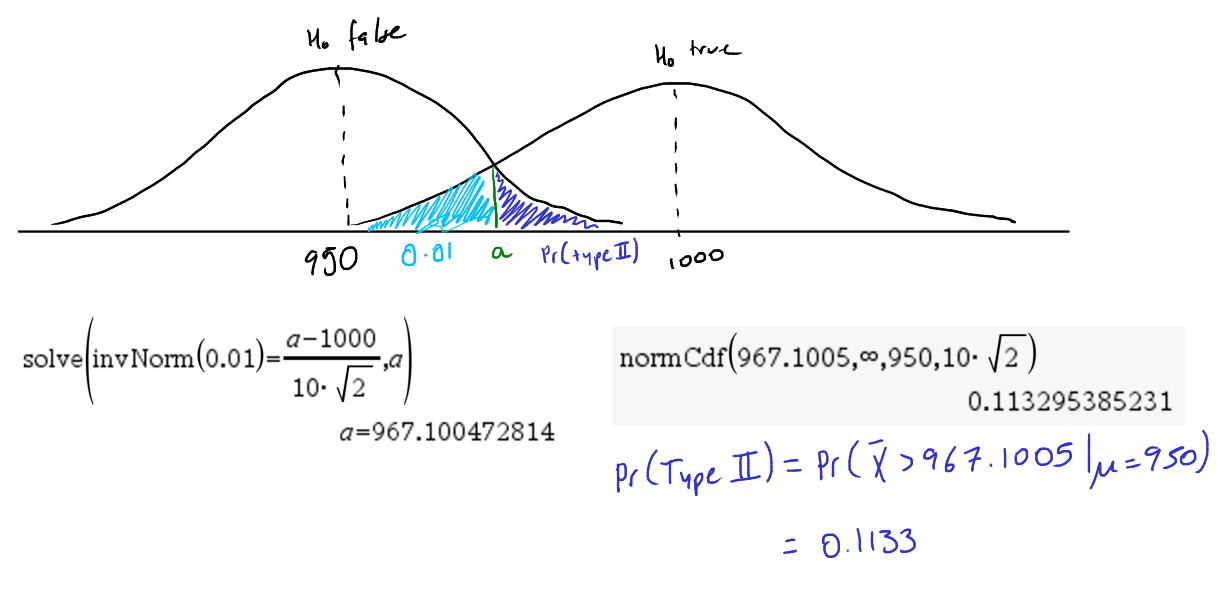
\includegraphics[width=\textwidth]{./img/heff2023speca20.png}
				\end{examquestion}
			
			\begin{examquestion}{VCAA 2021 Specialist E2 QB6}
				\begin{leftbar}
					The maximum load of a lift in a chocolate company's office building is 1000kg. The masses of employees who use the lift are normally distributed with a mean of 75kg and a standard deviation of 8kg. On a particular morning there are $n$ employees who use the lift.\\
					a) What is the maximum possible value of $n$ for there to be a less than 1\% chance of the lift exceeding the maximum load? (2 marks)
				\end{leftbar}
				\begin{align*}
					W\sim \mathrm{N}(75,8) &\qquad \text{Let }W_i\text{ be a random variable identically distributed to W},\quad T=\sum\limits_{i=1}^{n}W_i\\
					\E(T)=75n&\qquad \mathrm{sd}(T)=8\sqrt{n}\implies T\sim\mathrm{N}(75n,8\sqrt{n})\\
					\Pr\left(T<1000\right)&=\Pr\left(Z<\frac{1000-75n}{8\sqrt{n}}\right)>0.99\\
					\frac{1000-75n}{8\sqrt{n}}&>2.3263\\
					\implies n&=12 \text{ (nearest integer)}
				\end{align*}
				\begin{leftbar}
					Clare, who is one of the employees, likes to have a hot drink after she exits the lift. The time taken for a drink to be dispensed from the hot drink machine is normally distributed with a mean of 2 minutes and a standard deviation of 0.5 minutes. Time taken to dispense successive drinks are independent.\\
					b) Clare has a meeting at 9:00am and at 8:52 am she is fourth in the queue for a hot drink. Assume that the waiting time between hot drinks dispensed is negligible and that it takes Clare 0.5 minutes to get from the drink machine to the meeting room. What is the probability, correct to four decimal places, that Clare will get to her meeting on time? (2 marks)
				\end{leftbar}
				\begin{align*}
					T&\sim\mathrm{N}\left(2,\frac{1}{2}\right)\\
					\Pr\left(4T+\frac{1}{2}<8\right)&=\Pr\left(4T<15/2\right)\\
					X&=4T\sim\mathrm{N}(8,1)\\
					\Pr\left(X>\frac{15}{2}\right)=0.3085
				\end{align*}
				\begin{leftbar}
					Clare is a statistician for the company. The number of chocolate bars sold daily is normally distributed with a mean of 60000 and a standard deviation of 5000. To increase sales, the company decides to run an advertising campaign. After the campaign, the mean daily sales from 14 randomly selected days is 63500. Clare has been asked to investigate whether the campaign was effective, and so she performs a one-tailed test at the 1\% level of significance.
					c)i) Write down a null and alternative hypothesis. (1 mark)
				\end{leftbar}
				\begin{equation*}
					H_0: \mu=60000\qquad H_1: \mu>60000
				\end{equation*}
				\begin{leftbar}
					ii) Determine the $p$ value, correct to 4 decimal places, for this test. (1 mark)
				\end{leftbar}
				\begin{equation*}
					S\sim\mathrm{N}(60000,5000)\qquad p=\Pr(\bar{S}>63500 | \mu=60000)=\Pr\left(Z>\frac{63500-60000}{\frac{5000}{\sqrt{14}}}\right)=0.0044
				\end{equation*}
				\textbf{Note: } Menu+6+7+1 can also conduct a $z$ test for this hypothesis.
				\begin{leftbar}
					iii) Giving a reason, state whether there is any evidence for the success of the campaign? (1 mark)
				\end{leftbar}
				p=0.0044<0.01, and therefore there is sufficient evidence to reject $H_0$ and conclude the campaign was effective.
				\begin{leftbar}
					d) Find the range of values for the mean daily sales of another randomly selected 14 days that would lead to rejecting the null hypothesis at 1\% level of significance.
				\end{leftbar}
				\begin{align*}
					\Pr\left(Z>\frac{\bar{x}-60000}{\frac{5000}{\sqrt{14}}}\right)\leq0.01\\
					2.3263\leq\frac{\bar{x}-60000}{\frac{5000}{\sqrt{14}}}\\
					\implies \bar{x}\geq63109
				\end{align*}
				\begin{leftbar}
					e) The advertising campaign has been successful to the extent that the mean daily sales is now 63000. Another test is conducted at 5\% significance level. Find the probability of the null hypothesis being incorrectly accepted, to 3 decimal places.
				\end{leftbar}
				\begin{align*}
					\Pr\left(Z>\frac{s-60000}{\frac{5000}{\sqrt{14}}}\right)=0.05&\implies s=62198.03\\
					\Pr\left(\bar{s}<62198.03 | \mu=63000\right)&=0.274
				\end{align*}
			\end{examquestion}
			\includepdf[pages={24,25}]{./pdf/2018e2.pdf}
			\includepdf[pages={22,23}]{./pdf/2019e2.pdf}
			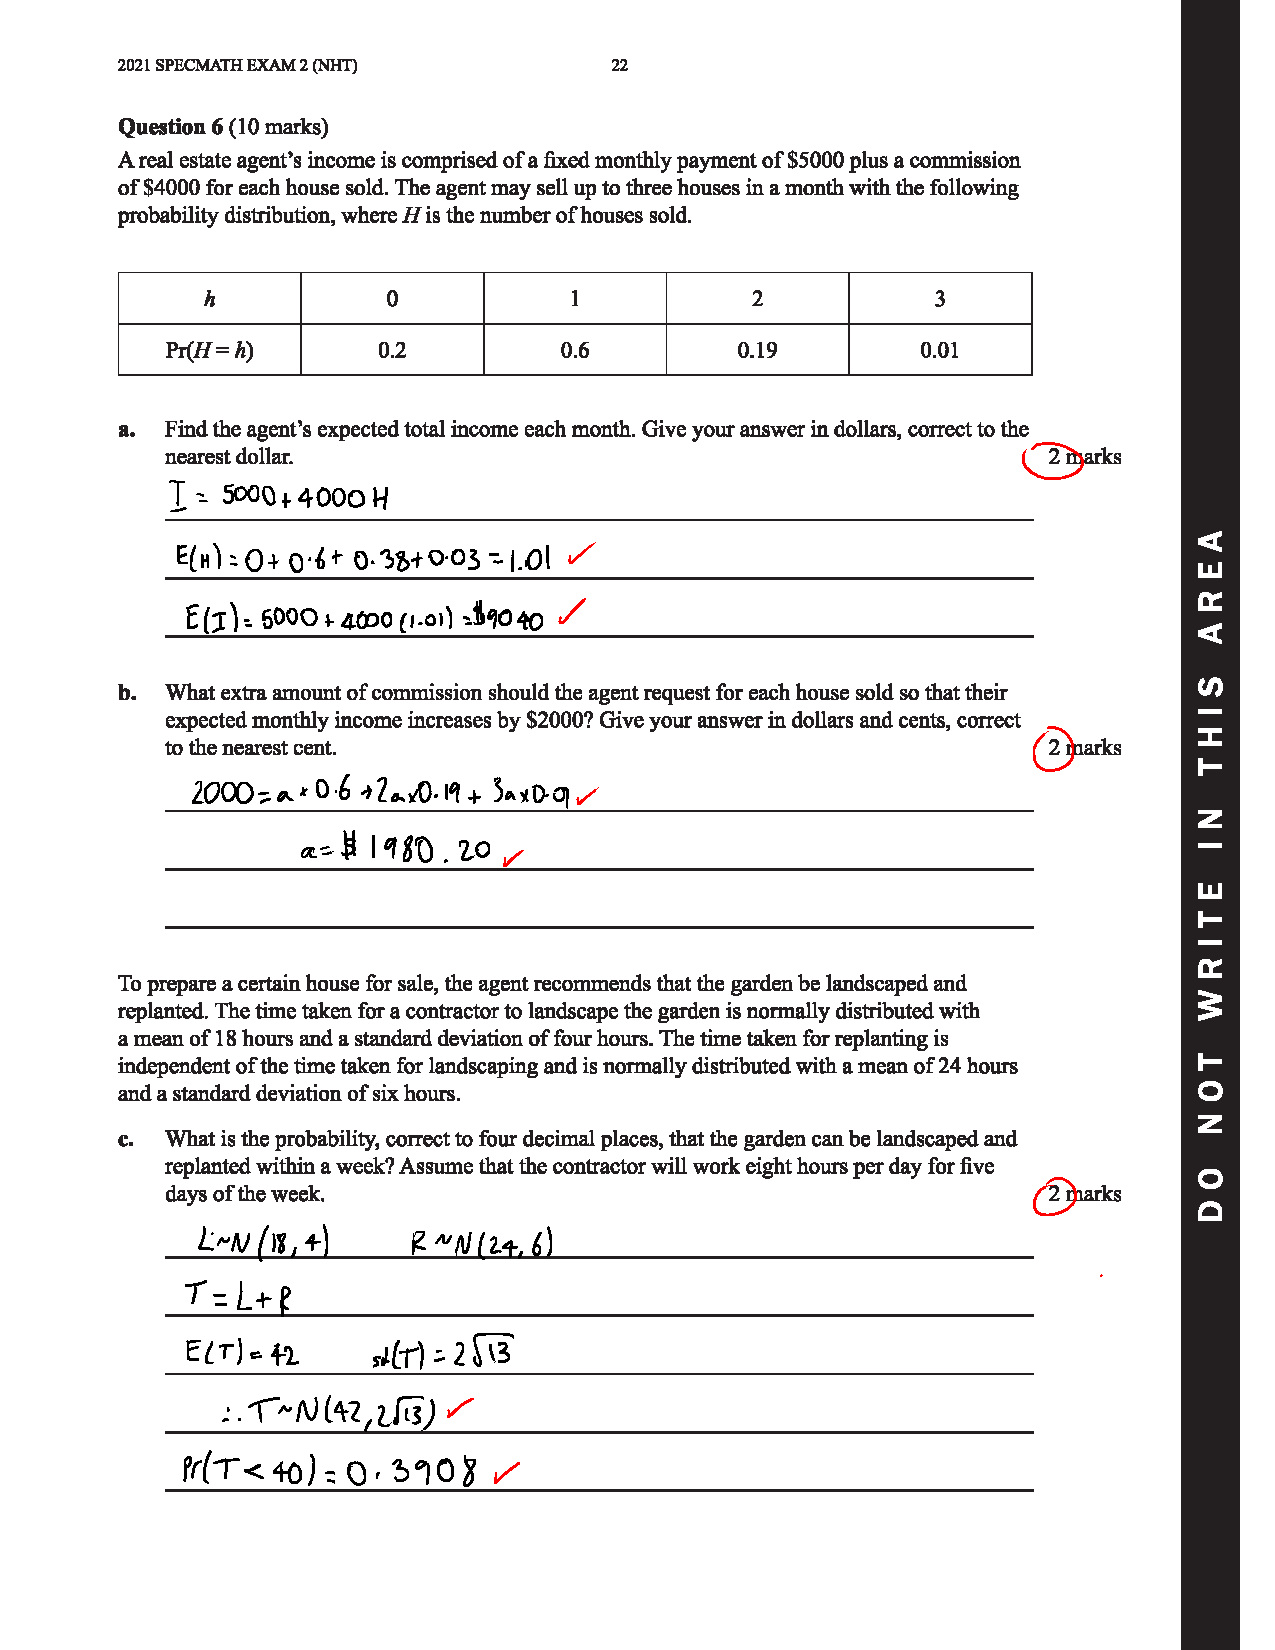
\includepdf[pages={1,2}]{./pdf/2021nhtsm2-stat.pdf}
			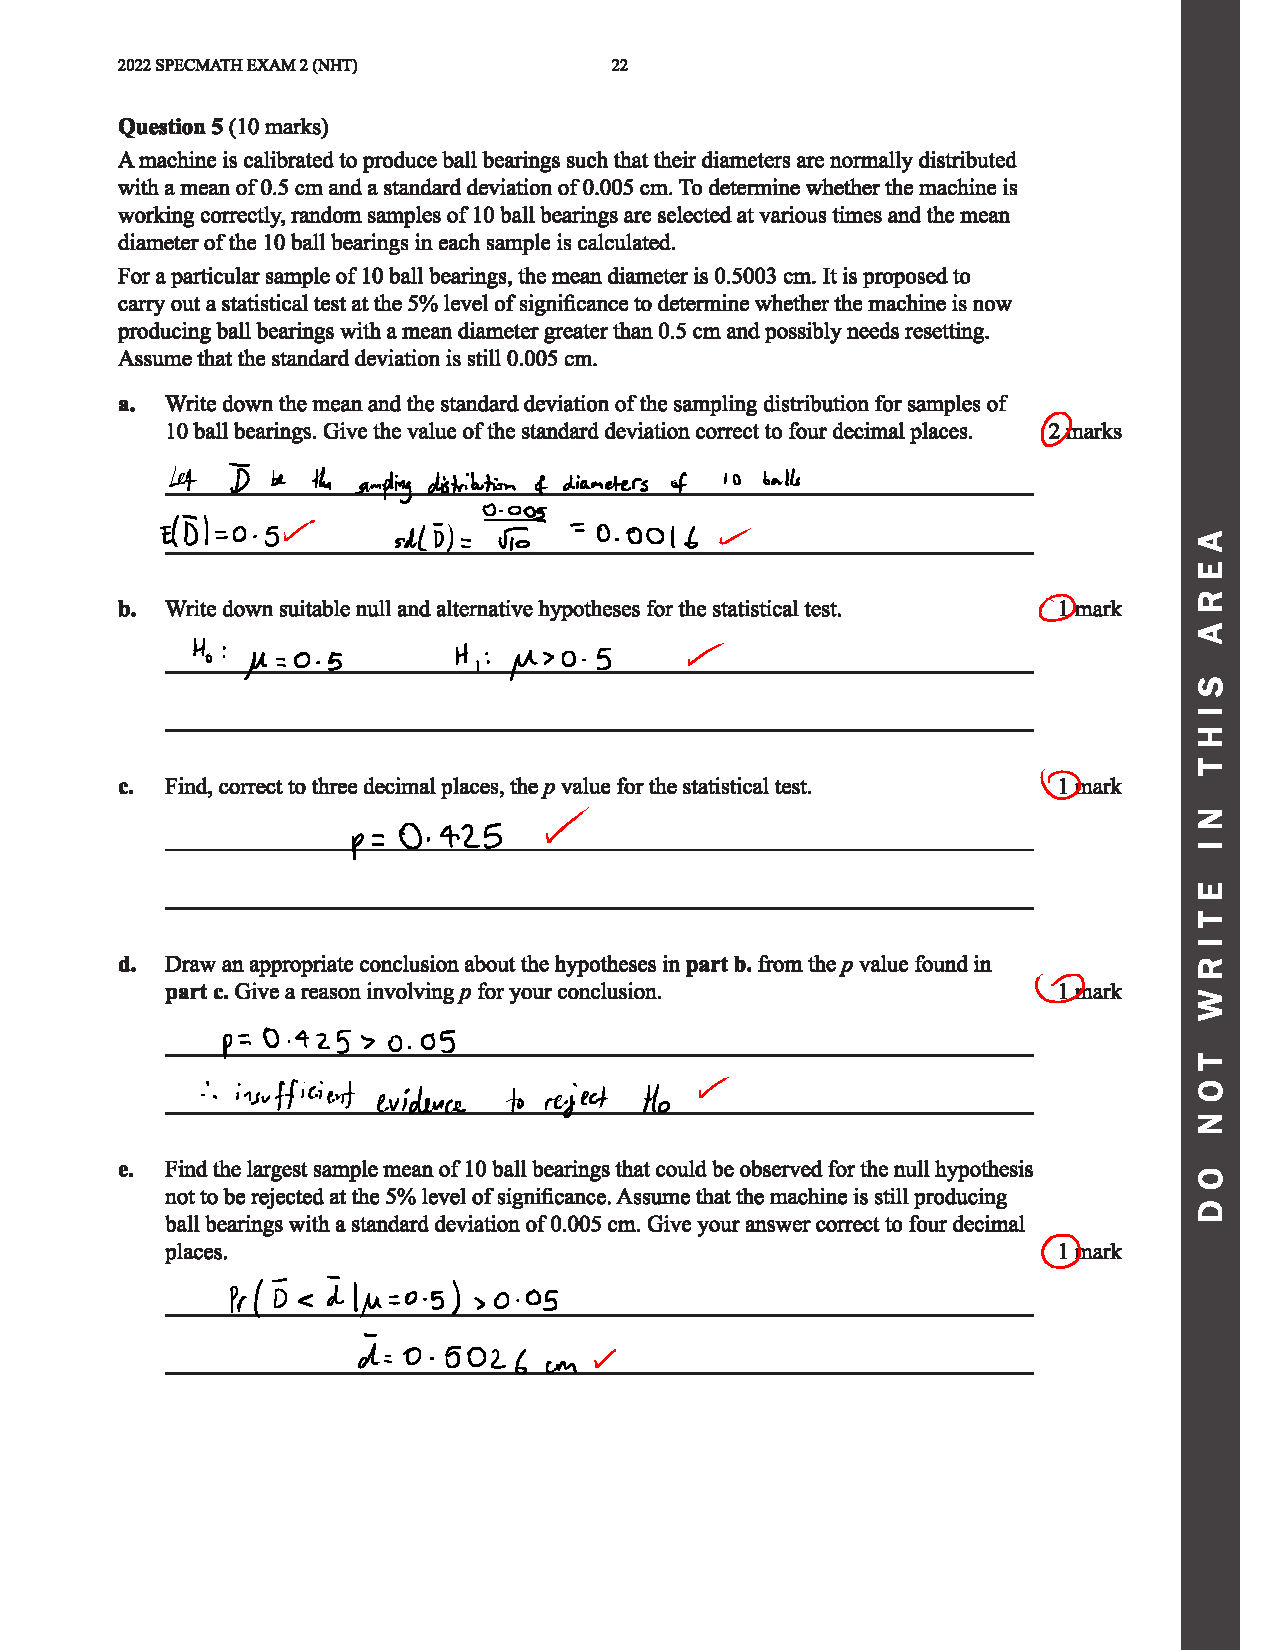
\includepdf[pages={1,2}]{./pdf/2022nhtsm2-stat.pdf}
	\section{Differential Calculus}			
		\subsection{Derivatives of x=f(y)}
			For $x=f(y)$ where $f$ is a one-to-one function:
			\[
				\frac{dy}{dx}=\frac{1}{\frac{dx}{dy}},\frac{dx}{dy}\neq0
			\]
		\subsection{Derivatives of Inverse Circular Functions}
		\subsection{Derivatives of Inverse Functions (Methods Doggery)}
			\paragraph{Theorem:} Let $f(x)$ be a function that is both invertible and differentiable. Let $y=g(x)$ be the inverse of $f(x)$.
			\[
				g'(x)=\frac{1}{f'(g(x))}
			\]
		\subsection{Second Derivatives}
		\subsection{Points of Inflection}
			\paragraph{Concavity test} must be completed to test all points of inflection, as $f''(x)=0$ does not necessarily mean it is a point of inflection, and concavity \textbf{must change.}
		\subsection{Related Rates}
		\subsection{Rational Functions}
			\subsubsection{Discontinuity - Vertical Asymptotes vs Holes}
				\paragraph{Holes} are also known as \textit{removable discontinuities} which occur when a factor in the denominator that equals 0 cancels with one in the numerator. Consider the following rational function:
				\[
					\frac{2x-6}{x^2-9}=\frac{2(x-3)}{(x+3)(x-3)}
				\]
				For $(x+3)(x-3)=0$, $x+3=0$ or $x-3=0$, but $x-3$ cancels in the numerator and denominator, so this is a removable discontinuity, or a 'hole'.
				\paragraph{Vertical Asymptotes} are known as \textit{non-removable discontinuities} which occur when a factor in the denominator that equals 0 can not be cancelled with one in the numerator. Consider the following rational function:
				\[
				\frac{2x-6}{x^2-9}=\frac{2(x-3)}{(x+3)(x-3)}
				\]
				For $(x+3)(x-3)=0$, $x+3=0$ or $x-3=0$, and $x+3$ does not cancel with any factors in the numerator, therefore when $x+3=0$ there is a vertical asymptote.
			\subsubsection{Diagonal Asymptotes}
			\begin{note}{Definition for diagonal asymptotes}
				A line $y=mx+c$ is a diagonal asymptote of $g(x)$ as $x\to\infty$ if $\lim\limits_{x\to+\infty}\left(g(x)-[mx+c]\right)=0$. Similarly when $\lim\limits_{x\to-\infty}\left(g(x)-[mx+c]\right)=0$. If $m=0$ then it is a horizontal asymptote.
			\end{note}
			\begin{examquestion}{2023 MAV Spec E2 QB5ai}
				\begin{leftbar}
					Consider the function:
					\[
					f_k: D_k\to\R,f_k(x)=\frac{x^2-1}{e^x-x-k},k\in\R
					\]
					where $D_k$ is the maximal domain of $f_k$.\\
					a) Let $k=2$\\
					i) $f_2$ has a diagonal asymptote $y=mx+c$. Find $m$ and $c$.
				\end{leftbar}
				\[
					\lim\limits_{x\to-\infty}f_2'(x)=-1=m
				\]
				Substitute $m=1$ into the definition:
				\begin{align*}
					&\lim\limits_{x\to-\infty}(f_2(x)-[-x+c])=0 &\implies \lim\limits_{x\to-\infty}(f_2(x)+x-c)=0\\
					&\implies \lim\limits_{x\to-\infty}(f_2(x)+x)=\lim\limits_{x\to-\infty}c=c &\implies c=2
				\end{align*}
				\textbf{Note:} $\lim\limits_{x\to\pm\infty}f'(x)$ may not exist when a diagonal asymptote exists.
			\end{examquestion}
			\begin{examquestion}{2023 MAV Spec E2 QB6bii}
				\begin{leftbar}
					Consider the function:
					\[
					f_k: D_k\to\R,f_k(x)=\frac{x^2-1}{e^x-x-k},k\in\R
					\]
					where $D_k$ is the maximal domain of $f_k$.\\
					b) ii) Find the value(s) of $k$ for which $f_k$ has two vertical asymptotes.
					
				\end{leftbar}
			\end{examquestion}
	\section{Integral Calculus}
		\subsection{Rules}
			\subsubsection{Definite Integral}
				The definite integral on interval $[a,b]$ denotes the signed area enclosed by the graph $y=f(x)$, the $x$-axis, and the lines $x=a$ and $x=b$.
				\[
					\int\limits_{a}^{b}f(x)dx=F(b)-F(a)
				\]
				where $F(x)$ is any antiderivative of $f(x)$
		\subsection{Inverse Circular Functions}
			\[
				\int\frac{1}{\sqrt{a^2-x^2}}dx=\arcsin\left(\frac{x}{a}\right)+c,x\in(-a,a)
			\]
			\[
				\int\frac{-1}{\sqrt{a^2-x^2}}dx=\arccos\left(\frac{x}{a}\right)+c,x\in(-a,a)
			\]
			\[
				\int\frac{a}{a^2+x^2}dx=\arctan\left(\frac{x}{a}\right)+c,x\in\R
			\]
		\subsection{u-Sub}
			\[
				\int f(u)\frac{du}{dx}dx=\int f(u)du
			\]
			\paragraph{Linear substitutions} Antiderivatives of expressions in the form $f(x)[g(x)]^n$ for a linear function $g$ can be found using linear substitution:
			\begin{examquestion}{}
				Evaluate $\int\limits_0^1xe^{-x^2}dx$.\\
				\begin{align*}
					\int\limits_0^1xe^{-x^2}dx&=\frac{1}{2}\int\limits_0^1(2x)e^{-x^2}dx \\
					&u=-x^2 \qquad \frac{du}{dx}=-2x \qquad x=0\implies u=0, x=1\implies u=-1 \\
					&=\frac{-1}{2}\int\limits_0^{-1}e^udu\\
					&=\frac{-1}{2}\left[e^u\right]_0^{-1} \\
					&=\frac{-1}{2}\left(e^{-1}-1\right)\\
					&=\frac{1}{2}-\frac{1}{2e}
				\end{align*}
			\end{examquestion}
			\begin{examquestion}{2006 NEAP E2 A11}
				\begin{leftbar}
					Using a suitable substitution, $\displaystyle \int\limits_0^{\frac{\pi}{4}}\left(\frac{\cos x}{\sin x+\cos^2 x}\right)dx$ can be expressed as:
				\end{leftbar}
				Let $u=\sin x$\\
				\begin{align*}
					\int\frac{\cos x}{\sin x+(1-\sin^2 x)}dx=\int\frac{1}{u+1-u^2}du
				\end{align*}
			\end{examquestion}
			\begin{examquestion}{}
				Using the substitution $u=\pi-x$,\\
				a) Show that $\displaystyle\int\limits_0^\pi\frac{x\sin x}{1+\cos^2x}dx=\int\limits_0^\pi\frac{(\pi-x)\sin x}{1+\cos^2x}dx$.\\
				\begin{align*}
					&u=\pi-x \qquad x=\pi-u \qquad \frac{du}{dx}=-1 \qquad du=-dx \\
					&\int\limits_{0}^{\pi}\frac{x\sin x}{1+\cos^2x}dx=\int\limits_{\pi}^{0}\frac{(\pi-u)\sin(\pi-u)}{1+\cos^2(\pi-u)}(-du)\\
					&=\int\limits_0^\pi\frac{(\pi-u)\sin(\pi-u)}{1+\cos^2(\pi-u)}du \\
					&=\int\limits_0^\pi\frac{(\pi-x)\sin(x)}{1+\cos^2x}dx \text{ (Because u is just a dummy variable)}
				\end{align*}
				b) Hence deduce that $\displaystyle\int\limits_0^\pi\frac{x\sin x}{1+\cos^2x}dx=\frac{\pi^2}{4}$.
				\begin{align*}
					&\int\limits_{0}^{\pi}\frac{x\sin x}{1+\cos^2x}dx=\int\limits_{0}^{\pi}\frac{\pi\sin x}{1+\cos^2x}dx-\int\limits_{0}^{\pi}\frac{x\sin x}{1+\cos^2x}dx \\
					2\int\limits_{0}^{\pi}\frac{x\sin x}{1+\cos^2x}dx&=\pi\int\limits_0^\pi\frac{\sin x}{1+\cos^2 x}dx\implies\int\limits_0^\pi\frac{x\sin x}{1+\cos^2x}dx=\frac{\pi}{2}\int\limits_0^\pi\frac{\sin x}{1+\cos^2x}dx\\
					&v=\cos x, dx=\frac{-1}{\sin x}du, x=0\to v=1, x=\pi\to v=-1 \\
					\pi\int\limits_0^\pi\frac{\sin x}{1+\cos^2 x}dx&=-\pi\int\limits_1^{-1}\frac{1}{1+u^2}du\\
					&=\pi\int\limits_{-1}^1\frac{1}{1+u^2}du=\pi\left[\arctan u\right]_{-1}^1 \\
					&=\frac{\pi^2}{2}\\
					&\therefore \int\limits_0^\pi\frac{x\sin x}{1+\cos^2 x}dx=\frac{1}{2}\cdot\frac{\pi^2}{2}=\frac{\pi^2}{4}
				\end{align*}
			\end{examquestion}
		\subsection{Integration by Trig Identities}
			Integrals of form $\displaystyle \int\sin^m(x)\cos^n(x)dx$ can be considered in three cases:
			\paragraph{Case 1: Power of sine is odd} If $m$ is odd, let $m=2k+1,k\in\mathbb{Z}$
			\[
				\sin^{2k+1}(x)=\left(\sin^2x\right)^k\sin x=(1-\cos^2x)^k\sin x
			\]
			We can then use the substitution $u=\cos x$ to evaluate integrals.
			\paragraph{Case 2: Power of cosine is odd} If $m$ is even and $n$ is odd, let $n=2k+1,k\in\mathbb{Z}$
			\[
				\cos^{2k+1}(x)=\left(\cos^2x\right)^k\cos x=(1-\sin^2x)^k\cos x
			\]
			We can then use the substitution $u=\sin x$ to evaluate integrals.
			\paragraph{Case 3: Both powers are even} If both $m$ and $n$ are even, we use the identities:
			\[
				\sin^2x=\frac{1}{2}\left(1-\cos(2x)\right)\qquad\cos^2x=\frac{1}{2}\left(1+\cos(2x)\right)\qquad\sin(2x)=2\sin(x)\cos(x)
			\]
			
			\paragraph{Products to Sums Identities} Recall the product to sum identities:
			\[
				2\cos x\cos y=\cos(x-y)+\cos(x+y) \qquad 2\sin x\sin y=\cos(x-y)-\cos(x+y) \qquad 2\sin x\cos y=\sin(x+y)+\sin(x-y)
			\]
			We can also use these for integration in appropriate questions.
		\subsection{Partial Fractions}
			\paragraph{Proper Fractions} If $g(x)$ and $h(x)$ are polynomials then $f(x)=\frac{g(x)}{h(x)}$ is a rational function. If the degree of $g$ is less than the degree of $h$ then $f(x)$ is a proper fraction.\\\\
			For \textbf{proper fractions}, we resolve into proper fractions with the following rules:
			\begin{itemize}
				\item For every linear factor $ax+b$ in the denominator, there will be a partial fraction of form $\frac{A}{ax+b}$
				\item For every repeated linear factor $(ax+b)^2$ in the denominator, there will be two partial fractions of form $\frac{A}{ax+b}$ and $\frac{B}{(ax+b)^2}$
				\item For every irreducable quadratic factor $ax^2+bx+c$ in the denominator, there will be a partial fraction of the form $\frac{Ax+B}{ax^2+bx+c}$.
				\item For every repeated irreducable quadratic factor $(ax^2+bx+c)^2$ in the denominator, there will be two partial fractions of form $\frac{Ax+B}{ax^2+bx+c}$ and $\frac{Cx+D}{(ax^2+bx+c)^2}$
			\end{itemize}
			For \textbf{improper fractions}, those where the degree of the numerator is greater than the denominator, we use polynomial division to first create a proper fraction then resolve as normal.
		\subsection{Integration by Parts}
			\[
				\int u\frac{dv}{dx}dx=uv-\int v\frac{du}{dx}dx
			\]
			\[
				\int\limits_{a}^{b}u\frac{dv}{dx}dx=\left[uv\right]_a^b-\int\limits_a^bv\frac{du}{dx}dx
			\]
			\begin{examquestion}{VCAA 2007 Spesh E2 B2}
				\begin{leftbar}
					Let $f(x)=x\arctan(x)$.\\
					a) Find $f'(x)$ and calculate the slope of $f$ at $x=0$.
				\end{leftbar}
				\begin{align*}
					f'(x)&=\arctan(x)+x\cdot\frac{1}{x^2+1}=\arctan(x)+\frac{x}{x^2+1}\\
					f'(0)&=0
				\end{align*}
				\begin{leftbar}
					d) Use the result for $f'(x)$ in part \textbf{a} to show that an antiderivative of $\arctan(x)$ is
					\[
						x\arctan(x)-\frac{1}{2}\ln(1+x^2)
					\]
				\end{leftbar}
				\begin{align*}
					f'(x)&=\arctan(x)+\frac{x}{x^2+1}\\
					\int f'(x)dx&=\int \frac{x}{x^2+1}dx+\int\arctan(x)dx\\
					\text{Let }u=1+x^2\qquad f(x)&=\int \arctan(x)dx+\frac{1}{2}\int\frac{1}{u}du\\
					\int\arctan(x)dx&=x\arctan(x)-\frac{1}{2}\ln(u)+c\\
					&=x\arctan(x)-\frac{1}{2}\ln(1+x^2)\text{ is an antiderivative as required}
				\end{align*}
			\end{examquestion}
		\subsection{Properties of the Definite Integral}
			\[
				\int\limits_a^bf(x)dx=\int\limits_a^cf(x)dx+\int\limits_c^bf(x)dx,a<c<b
			\]
			\[
				\int\limits_a^af(x)dx=0
			\]
			\[
				\int\limits_a^bkf(x)dx=k\int\limits_a^bf(x)dx
			\]
			\[
				\int\limits_a^bf(x)\pm g(x)dx=\int\limits_a^bf(x)dx\pm\int\limits_a^bg(x)dx
			\]
			\[
				\int\limits_a^bf(x)dx=-\int\limits_b^af(x)dx
			\]
		\subsection{Area Between Curves}
			Let $f$ and $g$ be continuous functions on the interval $[a,b]$ such that $\forall x\in[a,b] f(x)\geq g(x)$. The area of the region bounded between the two curves and the lines $x=a$ and $x=b$ can be found by evaluating:
			\[
				\int\limits_a^bf(x)dx-\int\limits_a^bg(x)dx=\int\limits_a^bf(x)-g(x)dx
			\]
			When the graphs intersect on the interval, you must evaluate an integral for each section.
		\subsection{Volumes of Solids of Revolution}
			By rotating a function around an axis you form a solid of revolution.
			\paragraph{Revolution around the x-axis} If the region being rotated is bounded by $y=f(x)$, $x=a$, $x=b$ and the $x$-axis, then:
			\[
				V=\pi\int\limits_a^bf(x)^2dx
			\]
			\paragraph{Revolution around the y-axis} If the region being rotated is bounded by $x=f(y)$, $y=a$, $y=b$ and the $y$-axis, then:
			\[
				V=\pi\int\limits_a^bf(y)^2dy
			\]
			\paragraph{Regions not bound by an axis} If the region to be rotated is bounded by two functions instead of by an axis, use the area between two curves form:
			\[
				V=\pi\int\limits_a^b(f(x))^2-(g(x))^2dx
			\]
		\subsection{Lengths of Curves in Plane}
			The length of a curve of $f(x)$ (for $f$ is differentiable and $f'$ is continuous) from $x=a$ to $x=b$ is given by:
			\[
				L=\int\limits_a^b\sqrt{1+\left(\frac{dy}{dx}\right)^2}dx=\int\limits_a^b\sqrt{1+\left(f'(x)\right)^2}dx
			\]
			
			\begin{examquestion}{VCAA Spesh 2017 E2 B3e}
				\begin{leftbar}
					A brooch is designed using inverse circular functions. The edges of the brooch in the first and third quadrants are described by these piecewise functions:
					\[
						\text{Q1: } f(x)=\begin{cases}
							3\arcsin\left(\frac{x}{2}\right)&0\leq x\leq\sqrt{2}\\
							3\arccos\left(\frac{x}{2}\right)&\sqrt{2}<x\leq 2
						\end{cases}\qquad
						\text{Q3: } g(x)=\begin{cases}
							-3\arccos(\frac{-x}{2})&-2\leq x<-\sqrt{2}\\
							-3\arcsin(\frac{-x}{2})&-\sqrt{2}\leq x\leq 0
						\end{cases}
					\]
					The graph of the whole brooch is shown below:\\
					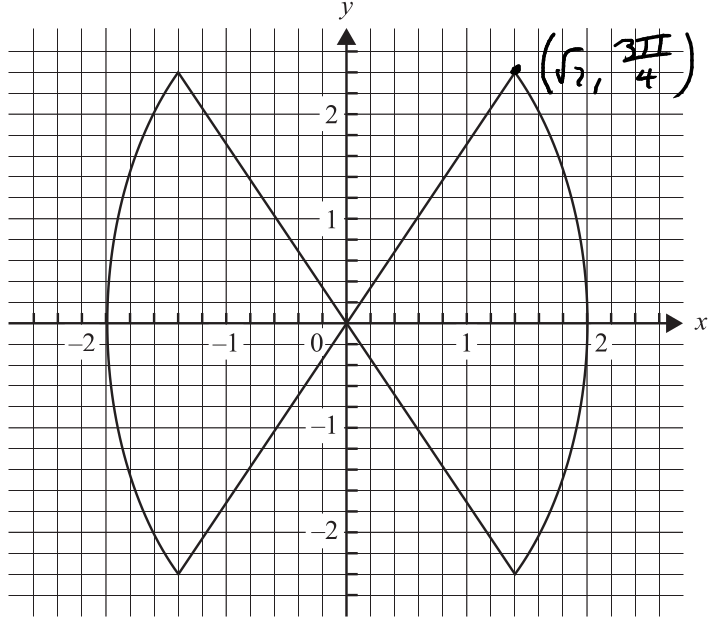
\includegraphics[width=0.5\linewidth]{2017e2b3.png}\\
					The perimeter of the brooch has a gold border. Show that the length of the gold border needed is given by a definite integral of the form $\displaystyle \int\limits_0^2\sqrt{a+\frac{b}{4-x^2}}dx$, where $a,b\in\R$. Find the values of $a$ and $b$.
				\end{leftbar}
				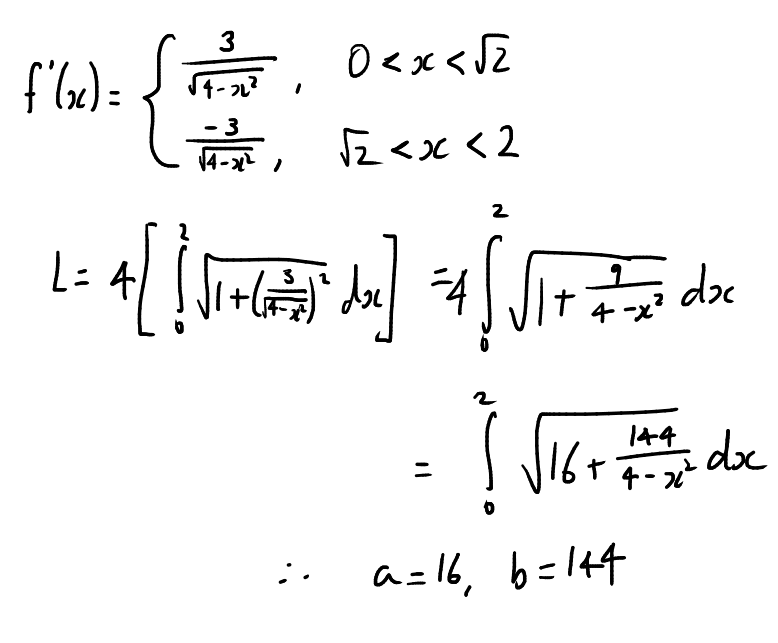
\includegraphics[width=0.4\linewidth]{2017e2b3eworking.png}
			\end{examquestion}
		\subsection{Areas of Surfaces of Revolution}
			\paragraph{Revolution About x-axis} If the region bounded by $y=f(x)$, the $x$-axis and $x=a$, $x=b$ is rotated about the x-axis, the area of the surface formed is given by:
			\[
				A=2\pi\int\limits_a^by\sqrt{1+\left(\frac{dy}{dx}\right)^2}dx
			\]
			
			\paragraph{Revolution About y-axis} If the region bounded by $x=f(y)$, the $y$-axis and $y=a$, $y=b$ is rotated about the y-axis, the surface area of the surface formed is given by:
			\[
				A=2\pi\int\limits_a^bx\sqrt{1+\left(\frac{dx}{dy}\right)^2}dy
			\]
			
			\paragraph{Surface Area of Parametrics} Consider a curve defined by $x=f(t)$ and $y=g(t)$ for $a\leq t\leq b$. If $P(f(t),g(t))$ traces the curve exactly once from $t=a$ to $t=b$ then the area formed by rotating about the $x$-axis is given by:
			\[
				A=2\pi\int\limits_a^b|g(t)|\sqrt{\left(\frac{dx}{dt}\right)^2+\left(\frac{dy}{dt}\right)^2}dt
			\]
			
			\paragraph{Total Surface Area of a Solid}
			\[
				\Sigma A=A+\pi\left(f(a)\right)^2+\pi\left(f(b)\right)^2
			\]
			For $A$ being the area of the surface, and $a,b$ being the limits of the solid of revolution.
		\subsection{Reduction Formulas}
			\begin{example}{Reduction Formulas Example 1}
				\[
					\text{Let } I_n=\int\limits_{1}^{e}(ln(t))^ndt\;n\in\mathbb{Z}^+
				\]
				i) Show that $I_n=e-nI_{n-1}$ for $n\in\mathbb{Z}^+$.\\
					\begin{align*}
						&I_n=\int\limits_{1}^{e}(ln(t))^ndt \\
						&u=(ln(t))^n \quad \frac{du}{dt}=\frac{n(ln(t))^{n-1}}{t} \quad \frac{dv}{dt}=1 \quad v=t \quad \text{(I.B.P)} \\
						&I_n=\left[t(ln(t))^n\right]_1^e-\int\limits_1^en(ln(t))^{n-1}dt \\
						&=e-n\int\limits_1^en(ln(t))^{n-1}dt \\
						&=e-nI_{n-1} \text{ As required}.
					\end{align*}
				ii) Hence, or otherwise, find the exact value of $I_3$.\\
					\begin{align*}
						I_3&=e-3I_2\\
						&=e-3(e-2I_1)=-2e+6(e-I_0) \\
						&=4e-6I_0=4e-6\int\limits_1^e(ln(t))^0dt=4e-\left[t\right]^e_1\\
						&=4e-6(e-1)=6-2e
					\end{align*}
			\end{example}
	\section{Differential Equations}
		\subsection{Tech}
			\subsubsection{deSolve(diffeq,iv,dv)} Press menu+4+D to get this function up. In the diffeq, denote derivatives with an apostrophe, iv is the independent variable and dv is the dependent variable.
			
			\subsubsection{euler(dydx,iv,dv,\{x0,x1\},y0,h)} Input the euler method function. dydx is the derivative of the dependent variable (dv) w.r.t the independent variable (iv). x0 is the x value stipulated in the initial condition, x1 is the maximum x value you wish to enumerate to. y0 is the y value in the initial condition and h is the step size.
		\subsection{Verification of Solutions}
			We can verify solutions to DiffEqs by substitution.
		\subsection{Proportionality/Inverse Proportionality}
			\begin{examquestion}{VCAA 2007 Spesh E2 A14}
				\begin{leftbar}
					The rate at which a type of bird flu spreads throughout a population of 1000 birds in a certain area is proportional to the product of the number $N$ of infected birds and the number of birds still \textbf{not} infected after $t$ days. Initially two birds in the population are found to be infected. A differential equation, the solution of which models the number of infected birds after $t$ days, is
				\end{leftbar}
				\textbf{\underline{My Blunder Solution}}:
				\[
					\frac{dN}{dt}=k(N-2)(1000-N)
				\]
				\textbf{\underline{Correct Solution}}:
				\[
					\frac{dN}{dt}\propto N(1000-N)\therefore \frac{dN}{dt}=kN(1000-N)
				\]
				The intiial value does not matter in this instance, as it is proportional to the product of the \textbf{currently} infected and non-infected birds, not the birds infected \textbf{since} the initial measurement.
			\end{examquestion}
		\subsection{Logistic DiffEq}
			\[
				\frac{dP}{dt}=rP\left(1-\frac{P}{K}\right)
			\]
			Where $P$ is the population at time $t$, $r$ is the 'growth parameter' (rate), $K$ is the upper limit of the population, $\frac{dP}{dt}\to0$ as $P\to K$. Maximum $\frac{dP}{dt}$ occurs at $P=\frac{K}{2}$.
			\paragraph{General Solution} The general solution to a logistic diffeq $\frac{dP}{dt}$:
			\[
				P(t)=\frac{P_0k}{P_0+(k-P_0)e^{-rt}}=\frac{P_0ke^{rt}}{P_0e^{rt}+(k-P_0)},\qquad P_0=P(0)
			\]
			\begin{examquestion}{VCAA 2023 Spesh Sample Q2}
				\begin{leftbar}
					In a certain region, 500 rare butterflies are released to maintain the species. It is believed that the region can support a maximum of 30 000 such butterflies. The butterfly population $P$, $t$ years after release can be modelled by the logistic differential equation $\displaystyle \frac{dP}{dt}=rP\left(1-\frac{P}{30 000}\right)$ where $r$ is the growth rate of the population.\\
					a) Use an integration technique and partial fractions to solve the DE above to find $P$ in terms of $r$ and $t$.\\
					b) Given that after 10 years there are 1930 butterflies, find $r$ to 2 decimal places.
				\end{leftbar}
				a)\\
				\begin{align*}
					r\frac{dt}{dP}=\frac{1}{P}+\frac{1}{30000-P}\\
					rt=\ln(P)-\ln(30000-P)+c,c\in\R\\
					P(0)=500\implies c=\ln(59)\\
					\therefore rt=\ln\left(\frac{59P}{30000-P}\right)\\
					P=\frac{30000}{1+59e^{-rt}}
				\end{align*}
				b)\\
				\begin{align*}
					P(10)=1930\\
					r=\frac{1}{t}\ln\left(\frac{59P}{30000-{}}\right)=\ln\left(\frac{59(1930)}{30000-1930}\right)\approx 0.14
				\end{align*}
			\end{examquestion}
			\begin{examquestion}{2023 MAV Spec E2 QA13}
				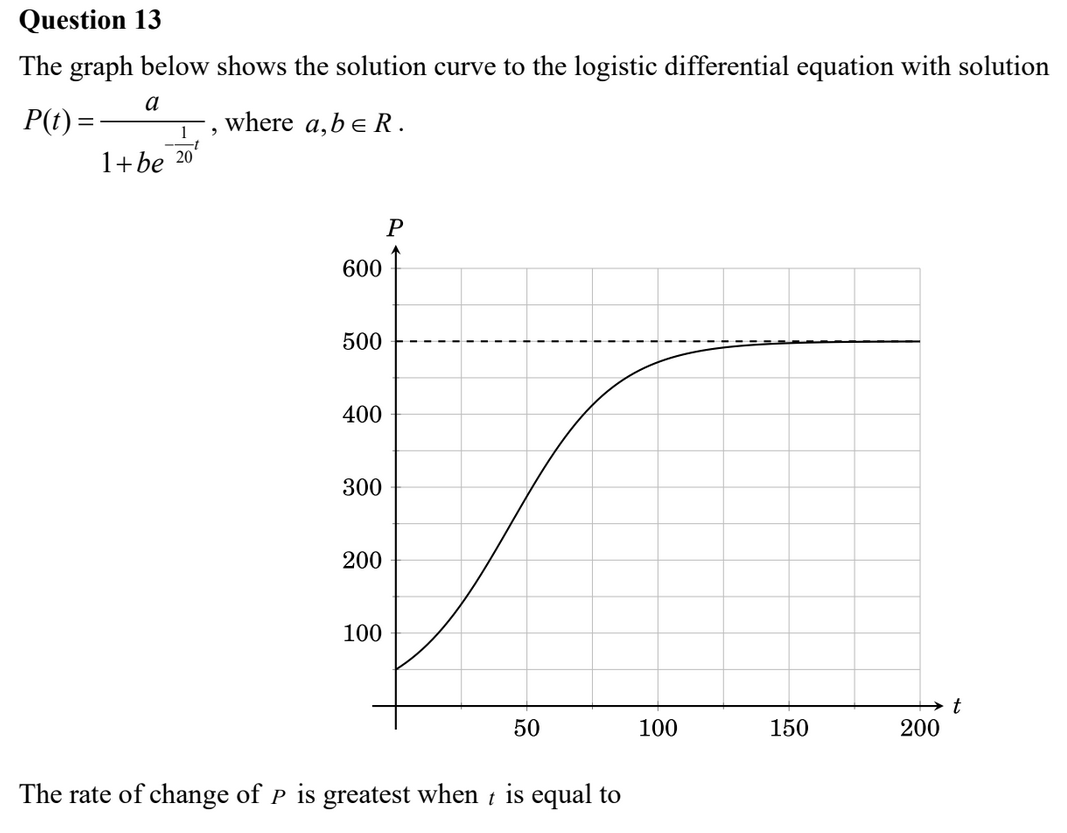
\includegraphics[width=\linewidth]{./img/mav2023specqa13.png}
				The asymptote is $P=500$ and so $a=500$.\\
				\[
					P(0)=\frac{500}{1+b}=50\implies b=9
				\]
				Solving $\frac{500}{1+9e^{-\frac{1}{20}t}}$ gives $t=20\ln(9)$.
			\end{examquestion}
		\subsection{Separation of Variables}
			\[
				\frac{dy}{dx}=f(x)g(y) \implies \int f(x)dx=\int\frac{1}{g(y)}dy
			\]
			\subsubsection{Solving}
				To solve $\displaystyle\frac{dy}{dx}=f(x)g(y)$:\\
				1) Write expression clearly as a product of a function in $x$ and a function in $y$.\\
				2) Substitute these expressions into the separation of variables form.\\
				3) Antidifferentiate both expressions with $+c$ included (you only need this on one side).\\
			\begin{examquestion}{2018 Exam 2 Question A9}
				A solution to the differential equation $\displaystyle \frac{dy}{dx}=\frac{2}{\sin(x+y)-\sin(x-y)}$ can be obtained from:\\
				a) $\displaystyle \int1dx=\int2\sin(y)dy$\\
				b) $\displaystyle \int\cos(y)dy=\int\csc(x)dx$\\
				c) $\displaystyle \int\cos(x)dx=\int\csc(y)dy$\\
				d) $\displaystyle \int\sec(x)dx=\int\sin(y)dy$\\
				e) $\displaystyle \int\sec(x)dx=\int\csc(y)dy$\\
				\begin{align*}
					\frac{dy}{dx}&=\frac{1}{\cos(x)\sin(y)} \\
					\sin(y)\frac{dy}{dx}&=\sec(x) \\
					\int\sin(y)dy&=\int\sec(x)dx \qquad \mathrm{(D)}
				\end{align*}
			\end{examquestion} 
		\subsection{DiffEqs + Related Rates Crossover Event}
			\begin{example}{Inverted Cone}
				An inverted cone has height $h$ and radius $r$. It is being filled at $k$ L per minute. The depth of the water is $x$ at time $t$ minutes. Construct a diffeq for $\frac{dx}{dt}$ and solve given the cone was initially empty.\\
				\begin{minipage}{0.6\textwidth}
					\begin{align*}
						&\text{Let }V\text{ be the volume of water after t minutes}\\
						&k\text{ litres}=1000k\mathrm{cm}^3\\
						&\frac{dV}{dt}=1000k\\
						&\frac{dx}{dt}=\frac{dx}{dV}\times\frac{dV}{dt}\\
						&V=\frac{1}{3}\pi y^2x\\
						\\
						&\text{By similar triangles: }\frac{y}{r}=\frac{x}{h}\implies y=\frac{xr}{h}\implies\qquad V=\frac{1}{3}\pi\frac{r^2x^2}{h^2}x=\frac{\pi r^2}{3h^2}x^3\\
						&\therefore \frac{dV}{dx}=\frac{\pi r^2}{h^2}x^2\implies\frac{dx}{dV}=\frac{h^2}{\pi r^2}\frac{1}{x^2}\therefore\frac{dx}{dt}=\frac{h^2}{\pi r^2x^2}\times1000k=\frac{1000kh^2}{\pi r^2x^2},k>0\\\\
						&t=\int\frac{\pi r^2 x^2}{1000kh^2}dx\\
						&=\frac{\pi r^2x^3}{3000kh^2}+c,c\in\R
					\end{align*}
					Then solve appropriately for $c$.
				\end{minipage}
				\hfill
				\begin{minipage}{0.2\textwidth}
					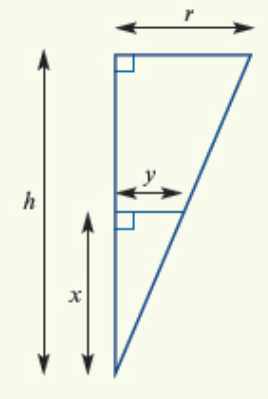
\includegraphics[width=\linewidth]{relatedratescone.png}
				\end{minipage}
				
			\end{example}
			
		\subsection{Definite Integration to solve DiffEqs}
			For differential equations $\frac{dy}{dx}=f(x)$ with $y_0=f(x_0)$ being known, the values of $y$ at $x_1$ can be found:
			\[
				y(x_1)=\int\limits_{x_0}^{x_1}f(x)dx+y_0
			\]
			\includepdf[pages={12-15}]{./pdf/2014e2.pdf}
		
		\subsection{Newton's Law of Cooling DiffEq} Newton's Law of Cooling involves a DiffEq that describes the rate of change of temperature $\frac{dT}{dt}$ is proportional to the difference between the temperature and the outside. Note that $k\in\R^-$ in the below statement.
		\[
			\frac{dT}{dt}\propto (T-T_{external})\implies\frac{dT}{dt}=k(T-T_{external})
		\]
		
		\subsection{Applications of DiffEqs - Concentration Problems}
			$Q$=concentration\\
			\[
				\frac{dQ}{dt}=\frac{dQ_{in}}{dt}-\frac{dQ_{out}}{dt}
			\]
			\textbf{In flow:} $\frac{dQ_{in}}{dt}=\frac{dQ_{in}}{dV_{in}}\times\frac{dV_{in}}{dt}$.\\
			\textbf{In tank:} Mass at any time $t$, volume at any time $t$, concentration $C=\frac{mass}{volume}$\\
			\textbf{Out flow:} $\frac{dQ_{out}}{dt}=\frac{dQ_{out}}{dV_{out}}\times\frac{dV_{out}}{dt}$. Out flowing concentration=concentration in tank $C$.
			
			\begin{examquestion}{2006 NEAP E1 A21}
				\begin{leftbar}
					A 5L container is initially full of fresh water. Saline solution with a concentration of 10g/L flows into the tank at 1L/min. At the same time, the mixture in the container flows out at 2L/min. If $S$ is the quantity of salt in the container at time $t$ minutes, write a differential equation describing this situation.
				\end{leftbar}
				\textbf{\underline{Into tank:}} $\displaystyle\frac{dQ_{in}}{dt}=10\times 1=10$\\
				\textbf{\underline{In tank:}} $\displaystyle C=\frac{S}{5+(1-2)t}=\frac{S}{5-t}$\\
				\textbf{\underline{Out of tank:}} $\displaystyle \frac{dQ_{out}}{dt}=\frac{S}{5-t}\times 2$\\\\
				Therefore $\frac{dS}{dt}=\frac{dQ_{in}}{dt}-\frac{dQ_{out}}{dt}=10-\frac{2S}{5-t}$
			\end{examquestion}
			
		\subsection{Euler's Method}
			If $\displaystyle\frac{dy}{dx}=g(x)$ with $y=y_0$ when $x=x_0$, then:
			\[
				x_{n+1}=x_n+h \qquad \text{and} \qquad y_{n+1}=y_n+hg(x_n)
			\]
			\begin{example}{Euler's Method Basic Case}
				\begin{leftbar}
					Let $\frac{dy}{dx}=x^2y$ with $y(1)=4$. Apply Euler's method to find $y_3$ using steps of $0.2$.
				\end{leftbar}
				\begin{align*}
					g(x,y)&=x^2y,\qquad h=0.2\\
					0:\qquad &x_0=1\qquad &y_0=4\\
					1:\qquad &x_1=1.2\qquad &y_1=4+0.2(1)^2(4)=4.8\\
					2:\qquad &x_2=1.4\qquad &y_2=4.8+0.2(1.2)^2(4.8)=6.18\\
					3:\qquad &x_3=1.6\qquad &y_3=6.18+0.2(1.4)^2(6.18)=8.606
				\end{align*}
			\end{example}
			\subsubsection{Over/Underestimates}
				If the graph of the solution of a DiffEq is concave up, Euler's Method will produce an underestimate. If the graph of the solution of a DiffEq is concave down, Euler's Method will produce an overestimate.
		\subsection{Slope Fields}
			\begin{examquestion}{2018 Exam 2 Question A10}
				The differential equation that best represents the slope field below is
				\begin{center}
					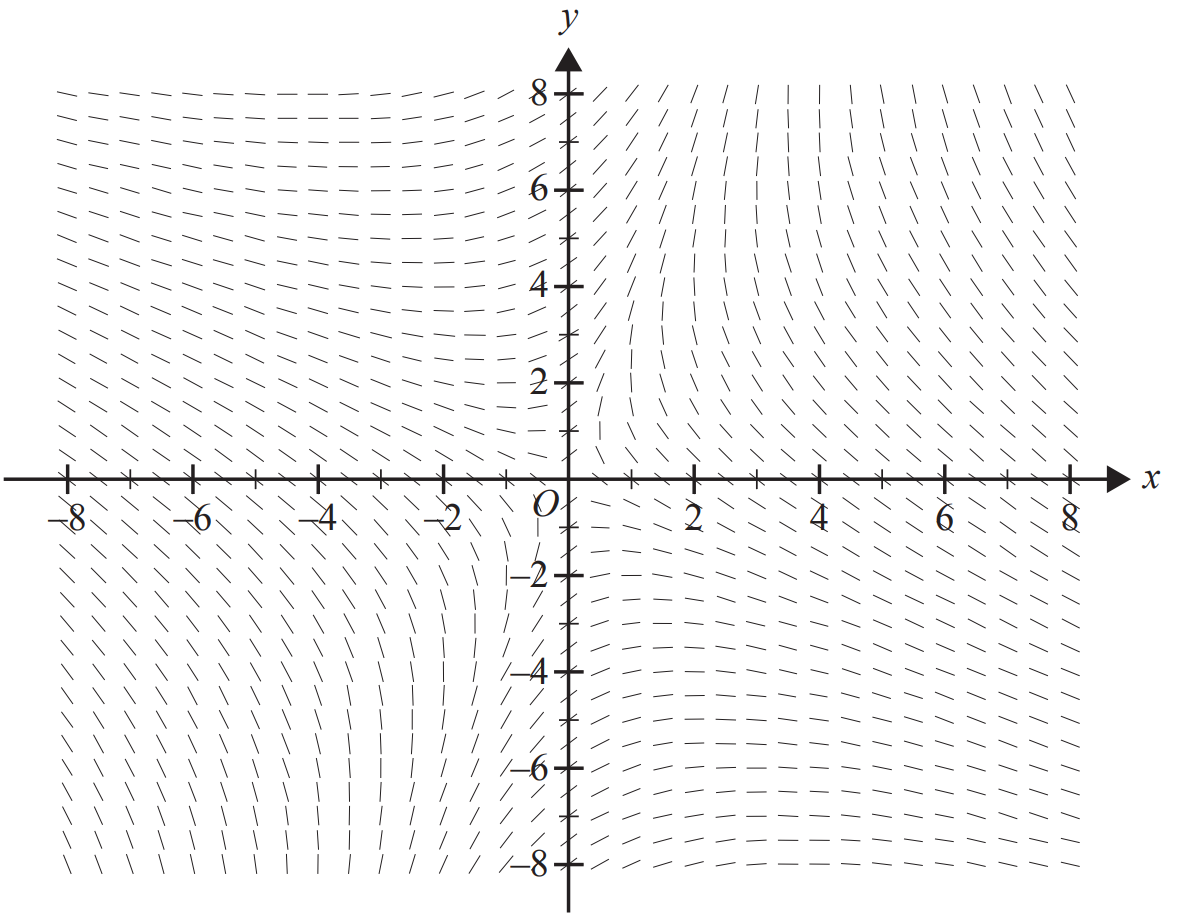
\includegraphics[width=8cm]{2018-2A10.png}\\
				\end{center}
				a) $\displaystyle \frac{dy}{dx}=\frac{2x+y}{y-2x}$\qquad b) $\displaystyle \frac{dy}{dx}=\frac{x+2y}{2x-y}$\qquad c) $\displaystyle \frac{dy}{dx}=\frac{2x-y}{x+2y}$\qquad d) $\displaystyle \frac{dy}{dx}=\frac{x-2y}{y-2x}$\qquad e) $\displaystyle \frac{dy}{dx}=\frac{2x+y}{2y-x}$\\\\
				Plot using \textbf{Graphs} page, Menu+3+8 to enter a diffeq. \textbf{A} has the same shape, so A is the answer.
			\end{examquestion}
		\subsection{Finding Solutions to DiffEqs}
			
	\section{Pseudocode}
		\subsection{Syntax}
			\paragraph{Assignment} A variable is a string of one or more letters that acts as a placeholder that can be assigned different values. For example $x\leftarrow3$ reads 'assign the value 3 to the variable $x$' or '$x$ takes the value 3'.
			
			\paragraph{Control of Flow of Steps}
				\subparagraph{If-Then Blocks} This construct provides a means of making decisions within an algorithm. If the condition is true, then the code between the If-Then block and the EndIf statement will execute.\\
				\textbf{If} \textit{condition} \textbf{then}\\
				\codeindent execute these instructions\\
				\textbf{End If}
				
				\subparagraph{For loops} Repeated execution of code blocks. Note the convention that 'from 1 to n' is inclusive.\\
				\textbf{For} \textit{i} \textbf{From} 1 \textbf{to} n\\
				\codeindent execute these instructions\\
				\textbf{End For}
				
				\subparagraph{While loops} Indefinite repeated iterations of instructions provided some condition remains true.\\
				\textbf{While} \textit{condition is true}\\
				\codeindent execute these instructions\\
				\textbf{End While}
				
			\paragraph{Functions} Functions are sections of pseudocode that can be used to complete a specific task. Once a function is defined it can be used ('called') within another algorithm.\\
			\textbf{define} \textit{function\textunderscore name}(args):\\
			\codeindent execute these instructions\\
			\textbf{return} output
		\subsection{Example Algorithms}
			\begin{example}{Newton-Raphson Method to tolerance of 0.001}
				\textbf{define} newtonraphson(f(x),x0)\\
				\codeindent df(x)$\leftarrow f'(x)$\\
				\codeindent i$\leftarrow0$\\
				\codeindent prevx$\leftarrow$x0\\
				\codeindent \textbf{While} i<1000 \textbf{do}\\
				\codeindent\codeindent nextx$\leftarrow$prevx - f(prevx) $\div$ df(prevx)\\
				\codeindent\codeindent \textbf{If} 0.001 < nextx - prevx < 0.001 \textbf{Then}\\
				\codeindent\codeindent\codeindent \textbf{Return} nextx\\
				\codeindent\codeindent \textbf{Else}\\
				\codeindent\codeindent\codeindent prevx$\leftarrow$nextx\\
				\codeindent\codeindent\codeindent i$\leftarrow$i+1\\
				\codeindent \textbf{EndWhile}
			\end{example}
			\begin{example}{Numerical Integration with Trapezium Method}
				\textbf{define} f(x)\\
				\codeindent \textbf{return} (function rule)\\\\
				sum$\leftarrow$0\\
				a$\leftarrow$lower bound\\
				b$\leftarrow$upper bound\\
				n$\leftarrow$number of trapeziums\\
				h$\leftarrow$(b-a)/n\\
				left$\leftarrow$a\\
				right$\leftarrow$a+h\\
				\textbf{for} i \textbf{from} 1 \textbf{to} n\\
				\codeindent strip$\leftarrow0.5($f(left)+f(right)$)\times h$\\
				\codeindent sum$\leftarrow$ sum + strip\\
				\codeindent left$\leftarrow$ left + h\\
				\codeindent right$\leftarrow$ right + h\\
				\textbf{end for}\\
				\textbf{print} sum
			\end{example}
			\begin{example}{Estimate of Long-Term Average for Number of Dice Rolls for a Six}
				sum$\leftarrow$0\\
				\textbf{for} i \textbf{from} 1 \textbf{to} 1000\\
				\codeindent outcome$\leftarrow$0\\
				\codeindent count$\leftarrow$0\\
				\codeindent\textbf{while} outcome $\neq$ 6\\
				\codeindent\codeindent outcome$\leftarrow$randominteger(1,6)\\
				\codeindent\codeindent count$\leftarrow$count + 1\\
				\codeindent\textbf{end while}\\
				\codeindent sum$\leftarrow$sum + count\\
				\textbf{end for}\\
				\textbf{print} sum/1000 
			\end{example}
			\begin{example}{Bisection Method for x-intercepts}
				\begin{minipage}[t]{0.5\textwidth}
					\underline{Algorithm:}\\\\
					\textbf{define} f(x):\\
					\codeindent \textbf{return} (function rule)\\
					a$\leftarrow$lower guess\\
					b$\leftarrow$upper guess\\
					c$\leftarrow$(a+b)/2\\
					t$\leftarrow$tolerance\\
					\textbf{if} f(a)$\times$ f(b)>0 \textbf{then}\\
					\codeindent \textbf{print} "Incorrect initial estimates"\\
					\textbf{else}\\
					\codeindent \textbf{while} b-a>2$\times$ t\\
					\codeindent\codeindent \textbf{if} f(a)$\times$ f(c)<0 \textbf{then}\\
					\codeindent\codeindent\codeindent b$\leftarrow$c\\
					\codeindent\codeindent \textbf{else}\\
					\codeindent\codeindent\codeindent a$\leftarrow$c\\
					\codeindent\codeindent \textbf{end if}\\
					\codeindent\codeindent c$\leftarrow$(a+b)/2\\
					\codeindent\codeindent \textbf{endwhile}\\
					\textbf{print} c\\
					\textbf{end if}
				\end{minipage}
				\hfill
				\begin{minipage}[t]{0.4\textwidth}
					\underline{Comments:}\\\\
					Function f(x) is chosen. For example, $x^2-2$. Good choices for a and b are a=1 and b=2 as f(1)<0 and f(2)>0\\\\
					The \textbf{while} loop requires that we continue the iteration until the desired accuracy is reached.\\
					The \textbf{if} statement inside the loop ensures that we continue to choose values for which there is a sign difference. For each iteration an average of the new pair is determined.
				\end{minipage}				
			\end{example}
	\section{Other Tech}
		\subsection{Functions}
			\subsubsection{scriptedmath\textbackslash poi(f(x),x)} Gives stationary points, axes intercepts, straight-line asymptotes, and endpoints.
			\subsubsection{scriptedmath\textbackslash inv(f(x),pointX)} Finds $f^{-1}(x)$. If the function is not one-to-one it will restrict domain to contain the point where x=pointX.
			\subsubsection{sam\textunderscore other\textbackslash newtonraphson(f,g,e,n)} Uses the Newton-Raphson method to approximate roots. f is the function, the roots of which we are trying to estimate. g is the derivative function. e is the initial estimate, and n is the number of iterations.
		\subsection{Parametric Functions}
			\subsubsection{scriptedmath\textbackslash pder(vfunc, parameter)} For a vector function in form $[x(t) y(t)]$ and parameter $t$. This function will find $\frac{dy}{dx}$.
	\section{Advanced Maths}
		\subsection{The Derivative of f(x)=4x+1} This could be a tough one. It might be best to take an indirect approach. Let's start with what we know:
		\[
		f(x)=4x+1
		\]
		and make the problem simpler by translating it to a coordinate system I'm going to call "Laplace Space"
		\[
		\Laplace\{f(x)\}=\Laplace\{4x+1\}
		\]
		Next we should refer to our table of Laplace Transforms, to convert our functions in $x$ to functions in $s$.
		\[
		F(s)=\frac{4}{s^2}+\frac{1}{s}=\frac{s+4}{s^2}
		\]
		Now we're in "Laplace Space". The cool thing about "Laplace Space" is that integration becomes division and differentiation becomes multiplication. To find the derivative, we generally want to multiply everything by $s$.
		\[
		sF(s)=\frac{s+4}{s}
		\]
		In "Laplace Space", the derivative of a function is $sF(s)-f(0)$.
		\[
		sF(s)-f(0)=\frac{s+4}{s}-(4(0)+1)=\frac{s+4-s}{s}=\frac{4}{s}
		\]
		The left hand side of our equation is now the version of $f'(x)$ that exists in "Laplace Space". To find what our derivative is actually equal to, we need to convert everything back to "Cartesian Space"
		\[
		\Laplace^{-1}\{sF(s)-f(0)\}=\Laplace^{-1}\{\frac{4}{s}\}
		\]
		\[
		f'(x)=4
		\]
		And that's our answer, $f'(x)=4$. By taking a detour through "Laplace Space", we were able to treat this like an algebra problem and avoid all of that troublesome, limit-based calculus.
		\subsubsection{Our Table of Laplace Transforms}
			\bgroup
			\everymath{\displaystyle}
			\def\arraystretch{2.5}
			\begin{table}[H]
				\footnotesize
				\begin{tabular}[t]{|p{5cm}|c|}
					\hline
					1&$\frac{1}{s}$\\\hline
					$e^{at},a\in\R$&$\frac{1}{s-a}$\\\hline
					$t^n,n\in\mathbb{Z}^+$&$\frac{n!}{s^{n+1}}$\\\hline
					$\sqrt{t}$&$\frac{\sqrt{\pi}}{2s^{\frac{3}{2}}}$\\\hline
					$\sin(at),a\in\R$&$\frac{a}{s^2+a^2}$\\\hline
					$\cos(at),a\in\R$&$\frac{s}{s^2+a^2}$\\\hline
					$t\sin(at),a\in\R$&$\frac{2as}{(s^2+a^2)^2}$\\\hline
					$t\cos(at),a\in\R$&$\frac{s^2-a^2}{(s^2+a^2)^2}$\\\hline
					$\sin(at)-at\cos(at),a\in\R$&$\frac{2a^3}{(s^2+a^2)^2}$\\\hline
					$\sin(at)+at\cos(at),a\in\R$&$\frac{2as^2}{(s^2+a^2)^2}$\\\hline
					$t^ne^{at},a\in\R,n\in\mathbb{Z}^+$&$\frac{n!}{(s-a)^{n+1}}$\\\hline
				\end{tabular}
				\hfill
				\begin{tabular}[t]{|p{5cm}|c|}
					\hline
					$\cos(at)-at\sin(at),a\in\R$&$\frac{s(s^2-a^2)}{(s^2+a^2)^2}$\\\hline
					$\cos(at)+at\sin(at),a\in\R$&$\frac{s(s^2+3a^2)}{(s^2+a^2)^2}$ \\\hline
					$\sin(at+b),a,b\in\R$&$\frac{s\sin(b)+a\cos(b)}{s^2+a^2}$\\\hline
					$\cos(at+b),a,b\in\R$&$\frac{s\cos(b)-a\sin(b)}{s^2+a^2}$ \\\hline   
					$\sinh(at),a\in\R$&$\frac{a}{s^2-a^2}$\\\hline
					$\cosh(at),a\in\R$&$\frac{s}{s^2-a^2}$\\\hline
					$e^{at}\sin(bt),a,b\in\R$&$\frac{b}{(s-a)^2+b^2}$\\\hline
					$e^{at}\cos(bt),a,b\in\R$&$\frac{s-a}{(s-a)^2+b^2}$\\\hline
					$e^{at}\sinh(bt),a,b\in\R$&$\frac{b}{(s-a)^2-b^2}$\\\hline
					$e^{at}\cosh(bt),a,b\in\R$&$\frac{s-a}{(s-a)^2-b^2}$\\\hline
					$f(ct),c\in\R$&$\frac{1}{c}F(\frac{s}{c})$\\\hline
				\end{tabular}
				\caption{Laplace Transforms for Equations in $t$}
			\end{table}
			\everymath{}
			\egroup
		\subsection{Sandwich Theorem}
			Let $g(x)\leq f(x)\leq h(x)$ for all $x$ near $a$ and
			\[
				\lim_{x\to a}g(x)=\lim_{x\to a}h(x)=L
			\]
			Then
			\[
				\lim_{x\to a}f(x)=L
			\]
			The function $f$ is 'sandwiched' between $g$ and $h$.
	\newpage
	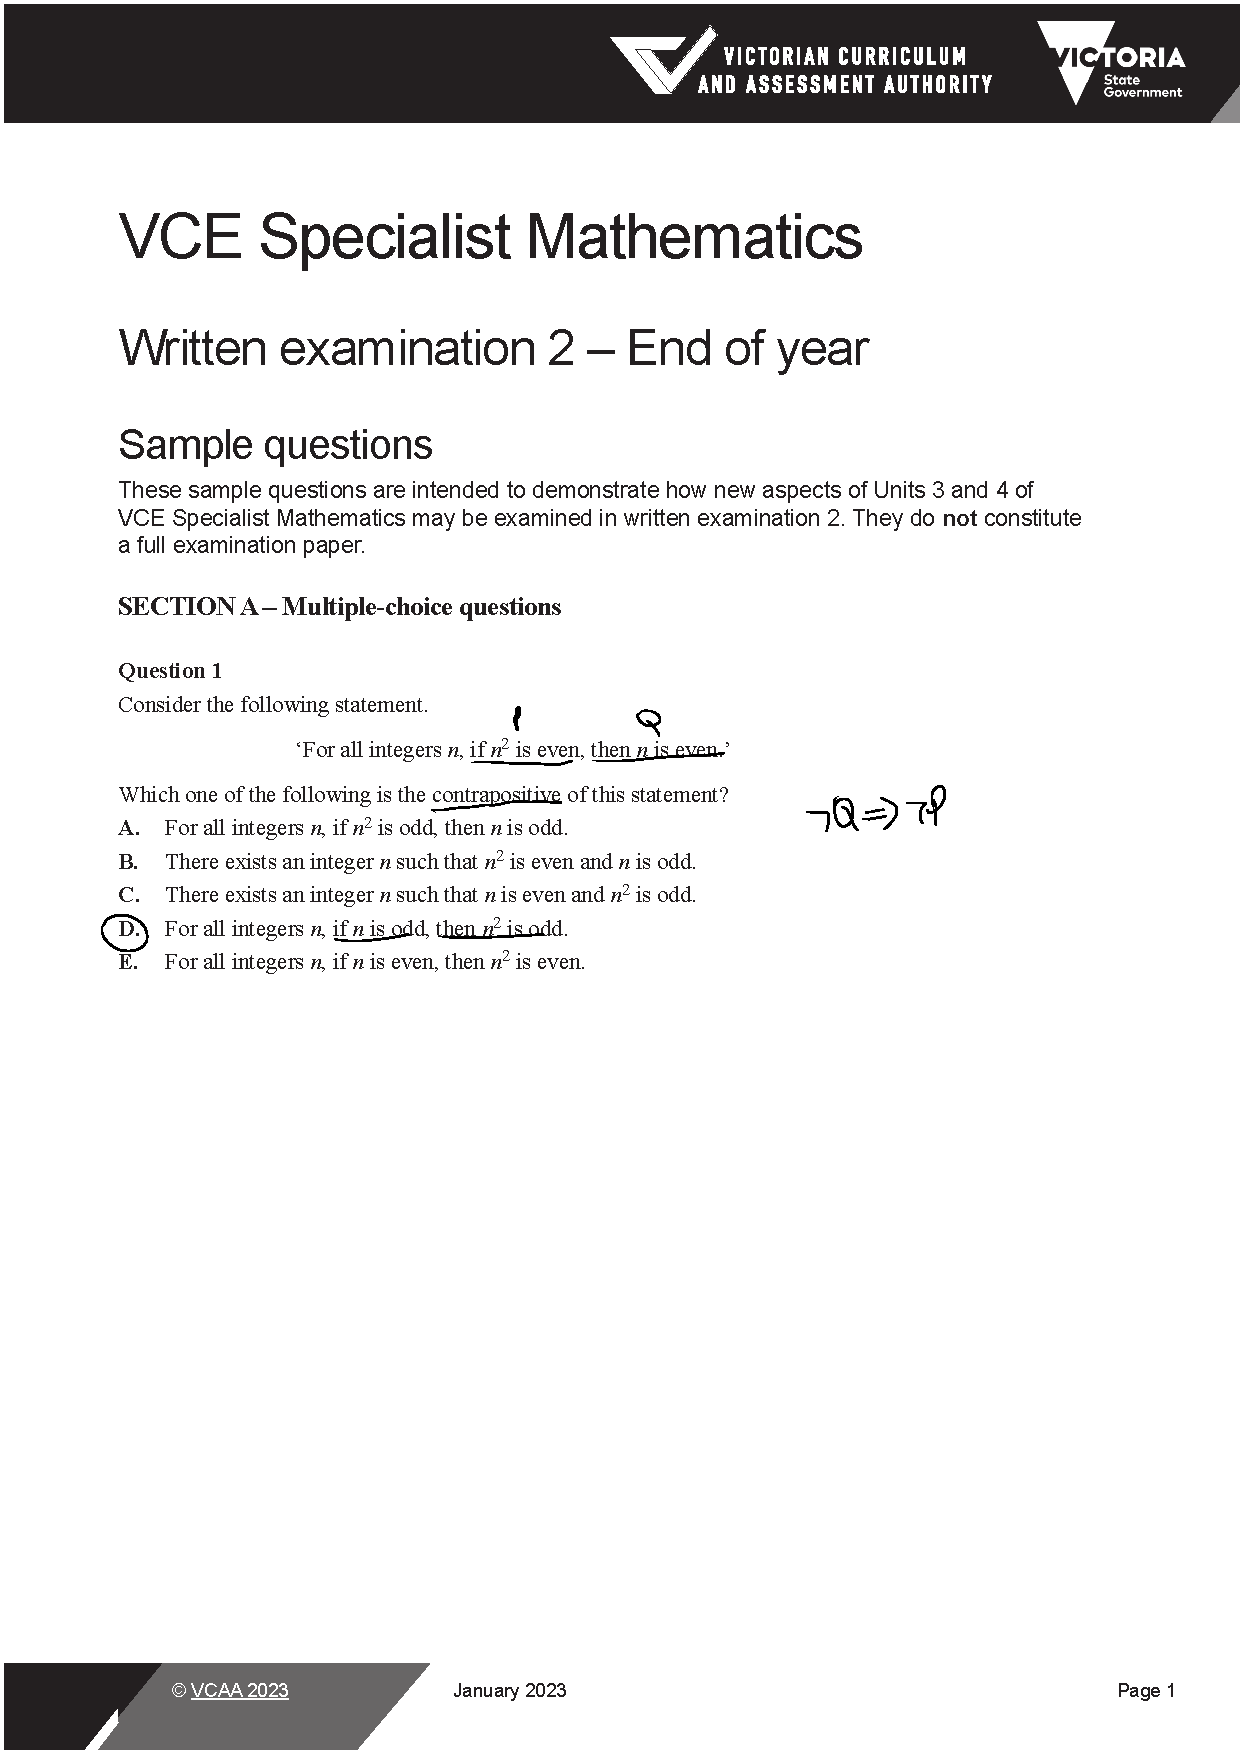
\includepdf[pages={1-14},scale=0.95,nup=2x2]{./pdf/2023SM2Sample.pdf}
	\section{Cheeky Snack}
\end{document}